% !TEX program = xelatex
\documentclass[UTF8,fontset=fandol,a4paper,11pt]{ctexart}
\usepackage[margin=21mm,top=23mm,bottom=22mm,headheight=16pt]{geometry}
\usepackage{amsmath,amssymb,mathtools,bm}
\usepackage{tikz}
\usetikzlibrary{arrows.meta,calc,angles,quotes,patterns}
\usepackage{xcolor,booktabs,array,longtable,enumitem,fancyhdr,needspace}
\usepackage[unicode,hidelinks]{hyperref}
\definecolor{ink}{HTML}{24343C}
\definecolor{accent}{HTML}{166A70}
\definecolor{muted}{HTML}{65747A}
\definecolor{rulegray}{HTML}{D4DDE0}
\definecolor{warm}{HTML}{966037}
\color{ink}
\setlength{\parindent}{2em}
\setlength{\parskip}{4pt}
\linespread{1.12}
\AtBeginDocument{\setlength{\abovedisplayskip}{6pt plus 2pt minus 1pt}
\setlength{\belowdisplayskip}{6pt plus 2pt minus 1pt}
\setlength{\abovedisplayshortskip}{0pt plus 1pt}
\setlength{\belowdisplayshortskip}{4pt plus 1pt}}
\setlist[enumerate]{label=(\arabic*),leftmargin=2.3em,itemsep=3pt,topsep=4pt}
\setlist[itemize]{leftmargin=2em,itemsep=2pt,topsep=4pt}
\allowdisplaybreaks[1]
\setlength{\emergencystretch}{2em}
\setcounter{secnumdepth}{0}
\providecommand{\tightlist}{\setlength{\itemsep}{0pt}\setlength{\parskip}{0pt}}
\ctexset{section={format=\Large\bfseries\color{accent},beforeskip=10pt,afterskip=9pt},
subsection={format=\normalsize\bfseries\color{accent},beforeskip=10pt,afterskip=4pt},
subsubsection={format=\normalsize\bfseries,beforeskip=8pt,afterskip=3pt}}
\pagestyle{fancy}
\fancyhf{}
\fancyhead[L]{\small\color{muted}物理学难题集萃}
% 页眉仅保留书名；版本名称只在封面显示。
\fancyfoot[L]{\small\color{muted}\chapterlabel}
\fancyfoot[R]{\small\thepage}
\renewcommand{\headrulewidth}{0.4pt}
\renewcommand{\footrulewidth}{0pt}
\newcommand{\dd}{\mathop{}\!\mathrm{d}}
\newcommand{\vect}[1]{\bm{#1}}
\newcommand{\tagline}[1]{\noindent{\small\color{muted}#1}\par}
\newcommand{\result}[1]{\begin{equation*}\boxed{#1}\end{equation*}}
\newcommand{\figcaption}[1]{\par\vspace{2pt}{\small\color{muted}#1}\par}
\newcommand{\teach}[2]{\Needspace{4\baselineskip}\subsection*{讲解要点与追问}#1\par\smallskip\noindent\textbf{追问：}#2\par}
\newcommand{\workarea}{\par\vspace{7mm}\noindent{\small\color{muted}作答区}\par\vspace{4mm}
\noindent\textcolor{rulegray}{\rule{\linewidth}{0.3pt}}\par\vspace{16mm}
\noindent\textcolor{rulegray}{\rule{\linewidth}{0.3pt}}\par\vspace{16mm}
\noindent\textcolor{rulegray}{\rule{\linewidth}{0.3pt}}\par\vspace{16mm}
\noindent\textcolor{rulegray}{\rule{\linewidth}{0.3pt}}}
\tikzset{axis/.style={-{Stealth[length=2mm]},thin,color=muted},
motion/.style={-{Stealth[length=2.3mm]},thick,color=accent},
force/.style={-{Stealth[length=2.3mm]},thick,color=warm},
traj/.style={thick,color=accent},guide/.style={dashed,thin,color=muted},
object/.style={thick,color=ink},every node/.style={font=\small}}\widowpenalty=10000\clubpenalty=10000\displaywidowpenalty=10000

\newcommand{\chapterlabel}{热学第三章\quad 气体动理论}
\hypersetup{pdftitle={热学第三章 气体动理论·学生解答版},pdfauthor={},pdfsubject={热学第三章第1--30题}}
\begin{document}
\pdfbookmark[0]{热学第三章 气体动理论}{cover}
\thispagestyle{empty}\vspace*{20mm}
\noindent{\Huge\bfseries 物理学难题集萃}\par\vspace{8mm}
\noindent{\LARGE 热学第三章}\par\vspace{5mm}
\noindent{\LARGE 气体动理论}\par\vspace{10mm}
\noindent{\Large\color{accent}学生解答版}\par\vspace{8mm}
\noindent\textcolor{accent}{\rule{\linewidth}{1pt}}\par\vspace{8mm}
\noindent 第1--30题\par\vspace{5mm}
\noindent 完整演算、图示分析与条件讨论。\par\vfill\clearpage
\pdfbookmark[1]{题目目录}{contents}\section*{题目目录}
\begin{longtable}{@{}>{\color{accent}\bfseries}r p{120mm}@{}}
\toprule 题号 & 题目\\\midrule
1 & 饱和蒸汽分子通量与蒸发速率比 \\
2 & 氯气分子反应冲量导致玻璃板偏转 \\
3 & 隔板推动试管后的最终速度 \\
4 & 一维小球气体的绝热压缩规律 \\
5 & 光子气压强、能量密度与绝热方程 \\
6 & 混合理想气体分子相对速率 \\
7 & 最概然平动能与最概然速率比较 \\
8 & 定容热气球升空后的振动与上升高度 \\
9 & 等温大气重力势能与热运动能量比 \\
10 & 大气压强随高度变化与半数分子高度 \\
11 & 等温大气分子的逃逸通量估算 \\
12 & 旋转封闭空气柱引起的液面上升 \\
13 & 等离子体在引力场中的电场平衡 \\
14 & 自由程分布函数与平均自由程 \\
15 & 分子随机游走位移与扩散时间 \\
16 & 混合气体中两类分子的平均自由程 \\
17 & 阴极射线管真空度与电子无碰撞概率 \\
18 & 球对称速度分布下的壁碰撞通量 \\
19 & 小孔逸出原子束的速率分布与衰减 \\
20 & 雨滴下落与飞虫平均自由程 \\
21 & 由细管流出测量气体粘滞系数 \\
22 & 线性热膨胀液体绝热混合体积不变 \\
23 & 湖冰增长估算冰的热传导率 \\
24 & 实心球与立方体冷却过程比较 \\
25 & 球壳稳态导热的温度分布与供能功率 \\
26 & 通电保险丝稳态温度分布 \\
27 & 绝热柱体非稳态热传导积分解 \\
28 & 小孔扩散导致左右气体密度随时间变化 \\
29 & 布朗粒子高度分布测阿伏伽德罗常数 \\
30 & 一维布朗运动位移方均量 \\\bottomrule\end{longtable}

\clearpage
% STUDY_GUIDE_BEGIN
\section*{本章学习安排}
本章把宏观热学与分子统计相连。先复习理想气体状态方程、动量冲量、立体角积分和常微分方程。第1--7题处理分子计数、辐射压及分布函数；第8--13题把玻尔兹曼权重用于高度分布与场中平衡；第14--21题讨论自由程、壁碰撞与束流；第22--30题转入导热和布朗运动。

读统计题时，先写清抽样对象：在空间内数分子、在孔口数出射事件、或在某一时间间隔数位移，权重各不相同。处理导热题先画控制微元并列流入、流出和储热，再选定温或绝热边界。第27题的反射热核与模态展开可在熟悉一维热方程后细读；积分式、边界条件、能量守恒和长时极限仍须相互核对。
% STUDY_GUIDE_END
\clearpage

\pdfbookmark[2]{第 1 题 饱和蒸汽分子通量与蒸发速率比}{q1}

\section*{第 1 题\quad 饱和蒸汽分子通量与蒸发速率比}

密闭容器中盛有未满的水，达到水与饱和水蒸气的平衡。14℃时饱和蒸气压为$12.0\,\mathrm{mmHg}$，100℃时为$760\,\mathrm{mmHg}$。水蒸气视为理想气体，分子碰到水面后均进入水内。求两温度下单位时间、单位水面面积蒸发的分子数之比$J_{100}:J_{14}$，取两位有效数字。

\begin{center}\begin{minipage}{0.96\linewidth}\centering\begin{tikzpicture}[x=1cm,y=1cm,font=\small,every node/.append style={align=center}]\fill[accent!15] (0,0) rectangle(5,1);\draw[object] (0,1)--(5,1);\node at (2.5,.4){水};\node at (2.5,2.6){饱和蒸气};\draw[motion] (1,1.1)--(1,2.1);\draw[force] (4,2.1)--(4,1.1);\end{tikzpicture}\figcaption{图 热3.1　水面上同时存在蒸发与凝结。}\end{minipage}\end{center}

\Needspace{8\baselineskip}\subsection*{解答}

平衡时蒸发与凝结的分子通量相等，分别记为$J_{\rm ev},J_{\rm co}$。水面上的蒸气数密度$n=p/(kT)$，各向同性分布给出
\[J_{\rm ev}=J_{\rm co}=\frac14 n\bar v,\qquad \bar v=\sqrt{\frac{8kT}{\pi m_w}}.\]
\begin{center}\begin{minipage}{0.96\linewidth}\centering\begin{tikzpicture}[x=1cm,y=1cm,font=\small,every node/.append style={align=center}]\fill[accent!15] (0,0) rectangle(5,1);\draw[object] (0,1)--(5,1);\node at (2.5,.4){水};\node at (2.5,2.6){饱和蒸气};\draw[motion] (1,1.1)--(1,2.1);\draw[force] (4,2.1)--(4,1.1);\node[left] at (1,1.7){$J_{\rm ev}$};\node[right] at (4,1.7){$J_{\rm co}$};\node at (2.5,1.65){$J_{\rm ev}=J_{\rm co}$};\end{tikzpicture}\figcaption{解图 热3.1A　平衡时两向分子通量相等；从凝结通量计算蒸发通量。}\end{minipage}\end{center}
解图热3.1A中向下箭头代表凝结通量，向上箭头代表蒸发通量；两支箭头都对应持续发生的过程，每单位面积、每单位时间离开与进入液面的分子数相等。
通量中的$1/4$来自方向投影。设速率概率密度为$f(v)$，与朝向水面的法线夹角为$\theta$。
时间$\dd t$内能到达面积$S$的分子，起点位于厚度$v\cos\theta\dd t$的斜柱中。
各向同性时方向概率为$\dd\Omega/(4\pi)$，所以
\[
\dd N=nf(v)\dd v\,\frac{\sin\theta\dd\theta\dd\phi}{4\pi}
Sv\cos\theta\dd t.
\]
对入射半球积分，
\[
J_{\rm co}=n\int_0^\infty vf(v)\dd v\,
\frac1{4\pi}\int_0^{2\pi}\dd\phi\int_0^{\pi/2}\cos\theta\sin\theta\dd\theta
=\frac{n\bar v}{4}.
\]
这里采用到达液面的分子均凝结的模型。因分子种类相同，$m_w$不变，故
\[J=\frac{p}{\sqrt{2\pi m_w kT}}\propto\frac p{\sqrt{T}}.\]
用$T_{100}=373.15\,\mathrm K,T_{14}=287.15\,\mathrm K$代入，压强可统一用mmHg：
\[\frac{J_{100}}{J_{14}}=\frac{760}{12.0}\sqrt{\frac{287.15}{373.15}}=55.56\ldots.\]
\result{J_{100}:J_{14}=56:1.}
蒸气压比约为63.3。升温使给定压强下的数密度下降、平均速率上升，合起来给压强比乘上 $\sqrt{T_{14}/T_{100}}$。若入水概率为相同的常数 $s<1$，两凝结通量同乘 $s$，比值保持。概率随温度变动时，比值再乘 $s_{100}/s_{14}$。
\subsubsection*{斜柱的法向厚度与两种温度效应}
解图热3.1B将方向投影单独画出。
在$\dd t$内碰到面积$S$的同一方向分子，初始位置属于沿速度方向回溯的斜柱；
斜柱在法线上的厚度为 $v\cos\theta\,\dd t$，于是体积为 $Sv\cos\theta\,\dd t$。垂直入射时 $\theta=0$，厚度为 $v\dd t$。
方向因子要同时包含入射半球限制和$\cos\theta$投影。

\begin{center}\begin{minipage}{0.96\linewidth}\centering
\begin{tikzpicture}[x=1cm,y=1cm,font=\small]
\fill[accent!10] (2.7,0)--(5.7,0)--(3.7,2)--(.7,2)--cycle;
\draw[object] (0,0)--(6.8,0);
\draw[guide] (2.7,0)--(.7,2)--(3.7,2);
\draw[motion] (3.7,2)--(5.7,0) node[midway,right] {$\vec v$};
\draw[guide] (3.7,2)--(3.7,.35);
\draw (3.7,1.4) arc(-90:-45:.6);
\node at (3.98,1.25) {$\theta$};
\draw[<->] (6.2,0)--(6.2,2) node[midway,right] {$v\cos\theta\,\dd t$};
\draw[<->] (2.7,-.4)--(5.7,-.4) node[midway,below] {$S$};
\node[above] at (2.2,2.15) {同方向分子的到达斜柱};
\node[left] at (0,0) {水面};
\end{tikzpicture}
\figcaption{解图 热3.1B　斜柱截面示意；计算到达数时用法向厚度，并对整个入射半球积分。}
\end{minipage}\end{center}
对速率的积分给$\bar v$，方向的积分给$1/4$，两者分开后才得到$n\bar v/4$。
这个结论只要求方向各向同性且速率与方向的统计分布可分离；
采用给定温度下的热平衡速率分布，进一步给$\bar v=\sqrt{8kT/(\pi m_w)}$。
比例系数与面积、容器体积无关，因此所求单位面积通量不会再乘容器总体积。

两温度间数密度和平均速率的比应分别列出：
\[
\frac{n_{100}}{n_{14}}=\frac{760}{12.0}\frac{287.15}{373.15}
\simeq48.74,\qquad
\frac{\bar v_{100}}{\bar v_{14}}=\sqrt{\frac{373.15}{287.15}}
\simeq1.140.
\]
速率比乘数密度比给通量比约55.56，压强比63.33进入了前面的数密度比。
若温度只按373 K和287 K取整，结果仍取两位有效数字为56。
压强在比值中采用同一单位即可约去；若要算绝对通量，则须将mmHg换成与$k$一致的SI压强。
$n$单位为$\mathrm{m^{-3}}$，$\bar v$单位为$\mathrm{m/s}$，
所以$J$单位为$\mathrm{m^{-2}s^{-1}}$，是分子数通量。

平衡时两向通量均为正，互相抵消而使 $J_{\rm ev}-J_{\rm co}=0$。题目比较的是向上的 $J_{\rm ev}$。同种液体在给定温度下的平衡蒸气压为 $p_s(T)$。若蒸气压低于这个值，而水面温度保持，实际凝结通量下降，出现净蒸发。


\Needspace{18\baselineskip}

\pdfbookmark[2]{第 2 题 氯气分子反应冲量导致玻璃板偏转}{q2}

\section*{第 2 题\quad 氯气分子反应冲量导致玻璃板偏转}

质量$m$的均匀薄玻璃板宽$2b$、高$c$，由两根等长细线悬挂；每根线长$2a$，上、下悬点的水平间距均为$2a$，两下悬点关于板的竖直中心轴对称。两表面的半面分别对称涂活泼金属：正面左半、背面右半。装置处在压强$p$的氯气中，每个氯气分子遇涂层发生反应的概率为$q<1$，反应分子被吸收，其余分子与表面完全弹性碰撞。两侧密度相同，反应引起的气压下降忽略。求玻璃板绕竖直中心轴的小平衡转角$\alpha$。细线质量及扭转弹性忽略。

\begin{center}\begin{minipage}{0.96\linewidth}\centering\begin{tikzpicture}[x=1cm,y=1cm,font=\small,every node/.append style={align=center}]\draw[object] (-1.8,3.6)--(1.8,3.6);\draw[object] (-1.8,3.6)--(-1.8,0);\draw[object] (1.8,3.6)--(1.8,0);\fill[accent!25] (-2.5,-1.4) rectangle(0,0);\draw[object] (-2.5,-1.4) rectangle(2.5,0);\draw[guide] (0,3.9)--(0,-1.7);\draw[<->] (-1.8,4.1)--(1.8,4.1) node[midway,above]{$2a$};\node[left] at (-1.8,1.8){$2a$};\draw[<->] (-2.5,-1.8)--(2.5,-1.8) node[midway,below]{$2b$};\node[right] at (2.5,-.7){$c$};\node at (-1.2,-.7){正面涂层};\node at (1.25,-.7){背面涂层};\end{tikzpicture}\figcaption{图 热3.2　正面左半、背面右半涂层；两下悬点距中心轴均为$a$。}\end{minipage}\end{center}

\Needspace{8\baselineskip}\subsection*{解答}

先算涂层改变了多少法向冲量。入射分子的法向速率为$|v_n|$，弹性反射传给板的冲量为$2m_c|v_n|$，吸收为$m_c|v_n|$。反应概率$q$与速度无关，碰撞通量相同，故
\[p'=(1-q)p+\frac q2p=\left(1-\frac q2\right)p,\qquad\Delta p=p-p'=\frac{qp}{2}.\]
\begin{center}\begin{minipage}{0.96\linewidth}\centering\begin{tikzpicture}[x=1cm,y=1cm,font=\small,every node/.append style={align=center}]\draw[object] (-2.5,0)--(2.5,0);\draw[accent,line width=3pt] (-2.5,.07)--(0,.07);\draw[warm,line width=3pt] (0,-.07)--(2.5,-.07);\draw[guide] (0,-1.5)--(0,1.5);\draw[force] (-1.25,-1.2)--(-1.25,-.1) node[pos=0,below]{$\Delta pbc$};\draw[force] (1.25,1.2)--(1.25,.1) node[pos=0,above]{$\Delta pbc$};\draw[<->] (0,.6)--(1.25,.6) node[midway,above]{$b/2$};\node[above] at (-2.8,1.2){俯视};\end{tikzpicture}\figcaption{解图 热3.2A　两个压强差作用在半面中心，形成同向转矩的力偶。}\end{minipage}\end{center}
解图热3.2A的俯视图中，正面左半和背面右半的压强差方向相反，形成力偶。每个半面面积$bc$，合力作用线过半面中心，离中心轴$b/2$。两力矩相加：
\[\tau_{\rm gas}=2(\Delta p\,bc)\frac b2=\frac12qp b^2c.\]
\textbf{细线的几何恢复力矩。} 两下悬点距轴均为$a$，转角$\alpha$后相对上悬点的水平偏移
\[d=2a\sin(\alpha/2)\simeq a\alpha.\]
每根线长$2a$，倾角$\beta$满足$\sin\beta=d/(2a)=\sin(\alpha/2)$，所以小角下$\beta\simeq\alpha/2$。竖直平衡给$2N\cos\beta=mg$。
\begin{center}\begin{minipage}{0.96\linewidth}\centering\begin{tikzpicture}[x=1cm,y=1cm,font=\small]
\draw[guide] (-2.5,0)--(2.6,0);
\draw[object] ({-2*cos(30)},{2*sin(30)})--({2*cos(30)},{-2*sin(30)});
\fill (0,0) circle(1.5pt) node[below left] {$O$};
\coordinate (C) at ({2*cos(30)},{-2*sin(30)});
\coordinate (S) at (2,0);
\draw[motion] (C)--(S) node[midway,right] {$N\sin\beta$};
\draw[motion] ({-2*cos(30)},{2*sin(30)})--(-2,0)
 node[midway,left] {$N\sin\beta$};
\fill (C) circle(1.5pt) node[below] {$C$};
\fill (S) circle(1.5pt) node[above right] {$S$};
\draw[<->] (0,.5)--(2,.5) node[midway,above] {$a$};
\draw (.85,0) arc(0:-30:.85);
\node at (1.04,-.23) {$\alpha$};
\node[align=left] at (-2.6,-.85) {$SC=d$\\顺时针偏转\\逆时针恢复};
\node[below] at (0,-1.6) {俯视；虚线为未偏转位置，示意角度放大};
\end{tikzpicture}\figcaption{解图 热3.2B　小角下$d\simeq a\alpha$、$\beta\simeq\alpha/2$；张力提供恢复转矩。}\end{minipage}\end{center}
解图热3.2B标出下悬点的水平偏移，悬线倾角另见解图热3.2C；水平张力的力臂为$a\cos(\alpha/2)$，两根线的恢复力矩为
\[\tau_{\rm res}=2Na\sin\beta\cos(\alpha/2)\simeq Na\alpha\simeq\frac12mga\alpha.\]
令两力矩大小相等，得
\result{\alpha=\frac{qpb^2c}{mga},\qquad\alpha\ll1.}
偏转也使玻璃板抬高。细线竖直投影为 $\sqrt{4a^2-d^2}$，板升高 $\Delta z\simeq d^2/(4a)=a\alpha^2/4$，于是 $\dd(mg\Delta z)/\dd\alpha=mga\alpha/2$。两式都把恢复系数联系到下悬点的横移距离。改变涂层位置时，按各半面的差压重新求合力和力矩。
\subsubsection*{用法向动量通量展开涂层压强}
设氯气单分子质量为$m_c$，入射法向速率$u>0$的一维概率密度为$g(u)$。
单位面积、单位时间到达的相应分子数为$nu g(u)\dd u$；
再乘单次法向冲量，弹性反射与吸收两种压强分别为
\[
p_{\rm el}=2nm_c\int_0^\infty u^2g(u)\dd u=p,\qquad
p_{\rm abs}=nm_c\int_0^\infty u^2g(u)\dd u=\frac p2.
\]
题设$q$与速度无关，所以吸收反应和未反应反射的贡献可分别写为
\[
p'_{\rm react}=\frac q2p,\qquad
p'_{\rm refl}=(1-q)p.
\]
二者相加得到$p'=(1-q/2)p$。
容器中的气体状态压强为 $p$。在涂层上，有些分子被吸收，每次只传递弹性反射时一半的冲量。因此，气体传给涂层的法向动量通量为 $p'$。

解图热3.2A中，左半面差压力向上、右半面向下，净力相消，转矩同为顺时针。
每个半面的力是$\Delta pbc$，两作用线相距$b$，
两支差压力等大反向，直接用其中一支力乘两力作用线之间的距离 $b$，得到 $\tau_{\rm gas}=(\Delta pbc)b$。
解图热3.2B按同一俯视方向画成顺时针偏转，
两根张力的水平分量均提供逆时针恢复转矩；两图采用同一俯视方向，恢复转矩与气体力矩相反。

\subsubsection*{悬线的竖直几何和小角近似的精度}
解图热3.2C单独画一根悬线所在的竖直平面。
U为固定上悬点，$C_0$为未转动时下悬点，C为转后的下悬点，
S是U在C所在水平面上的垂直投影。
$SC=d$是俯视图中同一弦长，而US为悬线的竖直投影。

\begin{center}\begin{minipage}{0.96\linewidth}\centering
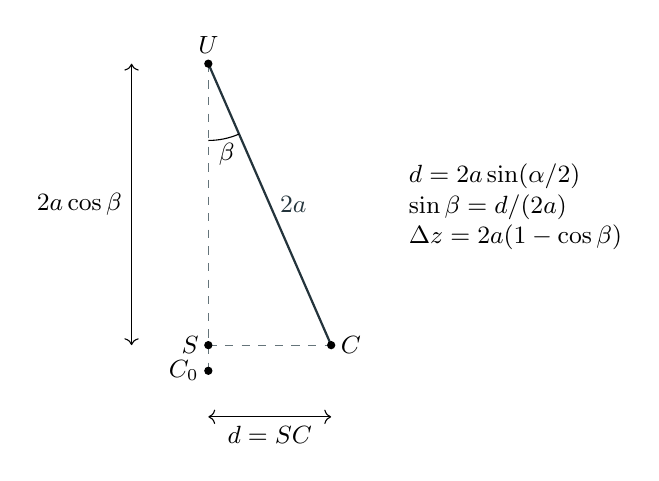
\begin{tikzpicture}[x=1.3cm,y=1.3cm,font=\small]
\coordinate (U) at (0,3);
\coordinate (C) at (1.2,{3-sqrt(9-1.44)});
\coordinate (S) at (0,{3-sqrt(9-1.44)});
\draw[guide] (U)--(0,0);
\draw[object] (U)--(C) node[midway,right] {$2a$};
\draw[guide] (S)--(C);
\draw[<->] (-.75,{3-sqrt(9-1.44)})--(-.75,3)
 node[midway,left] {$2a\cos\beta$};
\draw[<->] (0,-.45)--(1.2,-.45) node[midway,below] {$d=SC$};
\draw (0,2.25) arc(-90:-66.4218:.75);
\node at (.18,2.12) {$\beta$};
\fill (U) circle(1.5pt) node[above] {$U$};
\fill (0,0) circle(1.5pt) node[left] {$C_0$};
\fill (C) circle(1.5pt) node[right] {$C$};
\fill (S) circle(1.5pt) node[left] {$S$};
\node[align=left] at (3,1.6) {$d=2a\sin(\alpha/2)$\\$\sin\beta=d/(2a)$\\$\Delta z=2a(1-\cos\beta)$};
\end{tikzpicture}
\figcaption{解图 热3.2C　一根悬线的竖直截面；偏转使玻璃板升高，重力势能给恢复转矩。}
\end{minipage}\end{center}
在$0\le\alpha<\pi$的几何支上，$\beta=\alpha/2$。
不先作小角近似，由竖直平衡$N=mg/[2\cos(\alpha/2)]$代回，
\[
\tau_{\rm res}
=2Na\sin(\alpha/2)\cos(\alpha/2)
=mga\sin(\alpha/2)
=\frac12mga\alpha+O(\alpha^3).
\]
势能法同样给
\[
\Delta z=2a[1-\cos(\alpha/2)],\qquad
\frac{\dd(mg\Delta z)}{\dd\alpha}=mga\sin(\alpha/2).
\]
小角恢复力矩的系数由线长 $2a$ 和悬点半间距 $a$ 共同确定。其中 $1/2$ 来自悬线倾角与玻璃板转角的对应关系。
若仍采用各向同性气体、恒定$q,p$及相同涂层面积的模型，
气体力偶大小与板的水平转角无关，可进一步写
\[
\sin\frac\alpha2=\frac{qpb^2c}{2mga},\qquad
\alpha=2\arcsin\!\left(\frac{qpb^2c}{2mga}\right).
\]
小角近似要求$qpb^2c/(mga)\ll1$，
在这一范围内展开正弦式可得线性转角。若角度较大，按给定气体模型使用正弦关系，并在悬线有正竖直投影的几何支上求解。


\Needspace{18\baselineskip}

\pdfbookmark[2]{第 3 题 隔板推动试管后的最终速度}{q3}

\section*{第 3 题\quad 隔板推动试管后的最终速度}

真空中质量$M$的试管由质量$m$的隔板等分，封闭的下半管内装有$n$ mol、温度$T$、摩尔质量$\mu$的单原子理想气体。初始三者均静止。放开隔板后，它无摩擦地向管口移动，离开管口后气体才逸出。忽略重力及三者间热交换，隔板离管前的气体过程按准静态绝热处理。估算全部气体逸出后试管的最终速度，说明逸出阶段所用的分子冲量近似。

\begin{center}\begin{minipage}{0.96\linewidth}\centering\begin{tikzpicture}[x=1cm,y=1cm,font=\small,every node/.append style={align=center}]\draw[object] (0,3)--(0,0)--(2,0)--(2,3);\fill[accent!12] (0,0) rectangle(2,1.5);\draw[object,line width=2pt] (0,1.5)--(2,1.5);\node at (1,.7){$n,T,V$};\node[right] at (2.2,1.5){隔板$m$};\node[right] at (2.2,.2){试管$M$};\end{tikzpicture}\figcaption{图 热3.3　隔板初位于管长的一半；封闭气体在下半管。}\end{minipage}\end{center}

\Needspace{8\baselineskip}\subsection*{解答}

\textbf{隔板尚未离管。} 初始封闭气体体积记为$V$，隔板到管口时体积$2V$。按所给准静态绝热模型，$\gamma=5/3$，
\[TV^{2/3}=T_f(2V)^{2/3},\qquad T_f=2^{-2/3}T.\]
在共同后退的估算中，把试管及气体合并为质量$B=M+n\mu$的部分，后退速度大小$u_1$，隔板向前速度$v_p$。系统无外力，初始总动量零：
\[mv_p=Bu_1.\]
气体内能减少转为上述两部分的定向动能，
\[\frac32nR(T-T_f)=\frac12mv_p^2+\frac12Bu_1^2
=\frac{B(B+m)}{2m}u_1^2.\]
\begin{center}\begin{minipage}{0.96\linewidth}\centering\begin{tikzpicture}[x=1cm,y=1cm,font=\small,every node/.append style={align=center}]
\draw[object] (0,3)--(0,0)--(2.8,0)--(2.8,3);
\fill[accent!12] (0,0) rectangle (2.8,2.94);
\draw[guide] (0,1.5)--(2.8,1.5);
\node[left] at (-.1,1.5) {初始隔板位置};
\draw[object,line width=2pt] (0,3)--(2.8,3);
\node at (1.4,1) {$n,T_f,2V$\\$T_f=2^{-2/3}T$};
\node[right] at (3,3) {隔板$m$：到达管口};
\node[right] at (3,.2) {试管$M$};
\draw[motion] (4.5,1.8)--(4.5,2.8) node[right,midway] {$v_p$};
\draw[motion] (-2,1.2)--(-2,.2) node[left,midway] {$u_1$};
\node[above] at (1.4,3.7) {离管前：$V\longrightarrow 2V$};
\end{tikzpicture}\figcaption{解图 热3.3A\quad 隔板到达管口前，气体体积为$2V$、温度为$T_f$；$v_p$向上，$u_1$向下。}\end{minipage}\end{center}
解图热3.3A中，隔板的速度$v_p$向上，试管与尚未逸出气体的速度$u_1$向下。两部分总动量为零，故$mv_p=Bu_1$；能量式中的$B$也包括气体质量。隔板离管后转入解图热3.3B的开口逸出过程，气体质量开始减少。

消去$v_p$得
\[u_1=\sqrt{\frac{3mnR(T-T_f)}{(M+n\mu)(M+n\mu+m)}}.\]
\textbf{离管后的代表速率估算。} 从离管瞬间的状态出发，取以 $-u_1$ 匀速运动的惯性系。图中散开前朝底运动的半数分子各碰底一次，以一维方均根热速代表各分子的法向速率：
\[m_0=\frac{\mu}{N_A},\qquad v_{x,\rm rms}=\sqrt{\frac{kT_f}{m_0}}=\sqrt{\frac{RT_f}{\mu}}.\]
单次弹性碰撞冲量$2m_0v_{x,\rm rms}$，半数分子总冲量
\[P_{\rm rms}=\frac{nN_A}{2}\,2\frac\mu{N_A}\sqrt{\frac{RT_f}{\mu}}
=n\sqrt{\mu RT_f}.\]
\begin{center}\begin{minipage}{0.96\linewidth}\centering\begin{tikzpicture}[x=1cm,y=1cm,font=\small,every node/.append style={align=center}]\draw[object] (0,3)--(0,0)--(2,0)--(2,3);\draw[motion] (.5,1.7)--(.5,.15);\draw[motion] (.8,.2)--(.8,3.6);\draw[motion] (1.5,1.5)--(1.5,3.6);\node[left] at (0,.7){撞底};\node[right] at (2,2){向上者直接出管};\draw[force] (3,.8)--(3,-.1) node[right]{$P$};\end{tikzpicture}\figcaption{解图 热3.3B　一次碰底的代表速率模型：向下分子反射，给管底向后的冲量。}\end{minipage}\end{center}
于是该代表速率模型给出$u_2=P_{\rm rms}/M$，试管沿背离管口的方向运动：
\result{u\simeq\sqrt{\frac{3mnRT(1-2^{-2/3})}{(M+n\mu)(M+n\mu+m)}}
+\frac{n}{2^{1/3}M}\sqrt{\mu RT}.}
\textbf{统计平均及适用条件。} 第二项用了代表速率。改用初始麦克斯韦一维分布$g(v_x)$用于一次碰底模型，得
\[P=2nN_A m_0\int_{-\infty}^{0}|v_x|g(v_x)\dd v_x
=n\mu\langle|v_x|\rangle
=n\sqrt{\frac{2\mu RT_f}{\pi}}.\]
因此固定底面的一次碰撞平均会把第二项乘以$\sqrt{2/\pi}$。在 $n\mu\ll M$ 且一次碰底模型适用时，底面速度的变化相对热速很小，分子间后续碰撞也在本估算中略去。封闭阶段采用题设的准静态绝热假定。
\subsubsection*{先交代系统、参考系和两段的近似层次}
解图热3.3A以管口方向为正，离管前试管与隔板均可运动。
外界为真空，整个系统所受的外界压力功为零。气体在系统内部对隔板和管底做功。
封闭阶段的气体内能减少，可转为系统各部分的宏观定向动能；
把气体整体后退的动能与气体分子的无规则热运动内能分开计算。

第一段采用的估算还把气体整体后退速度视作与试管相同。
因此共同后退的质量写为 $B=M+n\mu$。准静态绝热式给出热运动的温度变化，共同后退是假定的宏观运动。若气体内部各处有不同的宏观速度，气体的整体动量和动能分别按局部速度和局部速度平方积分。

第二段改用一个以离管瞬间速度$-u_1$匀速运动的惯性系。
试管相对该系从静止开始，受到向后的分子冲量后速度变成 $-u_2$。参考系一直以 $-u_1$ 匀速移动。
变回初始实验室系，试管速度为$-(u_1+u_2)$，
所以最后所加的是两个同方向后退速率。
逸出期间还忽略分子间再碰撞、出管分子与隔板的后续碰撞，
以及管底反冲对碰底数目和相对入射速率的改变。
这些近似决定一次冲量模型所保留的过程。

\subsubsection*{封闭膨胀的温度、动量与能量全部展开}
隔板从管长一半移动到管口，气体体积从$V$变为$2V$。
单原子气体的$C_V=3R/2,\gamma=5/3$，
因此$T_f/T=2^{-2/3}$，剩余内能为$3nRT_f/2$，
释放到定向运动中的能量为
\[
\Delta U_{\rm released}
=\frac32nRT(1-2^{-2/3}).
\]
共同后退模型中，动量式给$v_p=Bu_1/m$。
代入动能式时逐项为
\[
\frac12mv_p^2+\frac12Bu_1^2
=\frac{B^2}{2m}u_1^2+\frac B2u_1^2
=\frac{B(B+m)}{2m}u_1^2.
\]
所以
\[
u_1^2=\frac{3mnRT(1-2^{-2/3})}
{(M+n\mu)(M+n\mu+m)}
=\frac{3(2^{2/3}-1)mnRT}
{2^{2/3}(M+n\mu)(M+n\mu+m)}.
\]
两种写法等价。动量 $Bu_1$ 和宏观动能 $Bu_1^2/2$ 中的后退质量均包括试管和气体。由 $v_p=Bu_1/m$ 求得隔板速度，两者动量大小相等，定向动能之和等于内能减少量。

\subsubsection*{逐个分子冲量的计数与统计平均}
离管前的热运动近似各向同性，
\[
\langle v_x^2\rangle=\langle v_y^2\rangle
=\langle v_z^2\rangle=\frac13\langle v^2\rangle,\qquad
\langle v^2\rangle=\frac{3RT_f}{\mu}.
\]
法向是三个等价分量之一，方均根为 $\sqrt{RT_f/\mu}$，即三维方均根的一份 $1/\sqrt3$。
解图热3.3B的代表速率模型把初始向下的半数分子视为各碰底一次，
向上的半数直接出管。单分子质量为$\mu/N_A$，
反射给管底冲量$2(\mu/N_A)\sqrt{RT_f/\mu}$，
总数$nN_A/2$相乘时阿伏伽德罗常量恰好约去，
得到$n\sqrt{\mu RT_f}$。
这项反冲只改变试管速度，用 $P_{\rm rms}/M$ 得该模型的速度增量 $u_2$。

如果使用同一初始热运动的完整一维分布，
令$\sigma=\sqrt{RT_f/\mu}$、$w=v_x/\sigma$，
\[
g(v_x)=\frac{1}{\sqrt{2\pi}\sigma}
\exp\!\left(-\frac{v_x^2}{2\sigma^2}\right),\qquad
\int_{-\infty}^{0}g(v_x)\dd v_x=\frac12.
\]
解图热3.3C中只有负速率分量对应初始朝底运动的分子，
对这半边取 $|v_x|$ 积分，反映各次入射冲量同向叠加。

\begin{center}\begin{minipage}{0.96\linewidth}\centering
\begin{tikzpicture}[x=1.15cm,y=4cm,font=\small]
\draw[axis] (-3.3,0)--(3.5,0) node[right] {$w=v_x/\sigma$};
\draw[axis] (0,0)--(0,.55) node[above] {$h(w)$};
\fill[accent!15,domain=-3:0,samples=80]
 (-3,0)--plot (\x,{exp(-.5*\x*\x)/sqrt(2*pi)})--(0,0)--cycle;
\draw[traj,domain=-3:3,samples=110]
 plot (\x,{exp(-.5*\x*\x)/sqrt(2*pi)});
\node at (-1.45,.26) {朝底，概率$1/2$};
\node at (1.6,.26) {朝管口};
\node[below] at (0,0) {0};
\end{tikzpicture}
\figcaption{解图 热3.3C　初始法向速度分布；一次碰底总冲量对负半轴按$|v_x|$加权。}
\end{minipage}\end{center}
在固定底面、忽略后续碰撞的近似内，
\[
P_{\rm mean}
=2n\mu\int_{-\infty}^{0}|v_x|g(v_x)\dd v_x
=2n\mu\frac{\sigma}{\sqrt{2\pi}}
=n\sqrt{\frac{2\mu RT_f}{\pi}}.
\]
因此
\[
u_{2,\rm mean}
=\frac n{2^{1/3}M}\sqrt{\frac{2\mu RT}{\pi}},
\qquad
\frac{P_{\rm mean}}{P_{\rm rms}}=\sqrt{\frac2\pi}\simeq0.7979.
\]
这里统计的是有限一批分子各碰一次的总冲量，
故用单侧速度的一阶矩；稳态气压还要按单位时间到达次数加权，
才出现速度的二阶矩。这里的有限批次由各分子的单次冲量直接求和。

\subsubsection*{管底反冲与末态动能}
固定底面反射保留每个分子的速率。有限质量的试管受到反冲后获得动能，这部分能量由气体转移。若管底速度显著，分子的相对入射速度随时间改变，部分较慢的分子会追不上后退的底面。$n\mu/M\ll1$ 时，底面的速度改变量相对热速小，单次固定底面冲量可作首阶估算。

末态动量确定后，可用质心动能求最低所需能量。
在第二段所取惯性系，若管底获得后退动量P，气体最终总动量为$+P$，
则两者末态的总动能至少为
\[
K_{\rm min}=\frac{P^2}{2M}+\frac{P^2}{2n\mu}.
\]
在一次碰底模型中，忽略气体与离管隔板的后续交换，第二段可用的初始气体内能为 $3nRT_f/2$，故要求 $K_{\rm min}\leq3nRT_f/2$。代代表速率冲量 $P_{\rm rms}=n\sqrt{\mu RT_f}$，得到必要条件 $1+n\mu/M\le3$。实际剩余的热运动会继续占用这笔能量。代表速率与分布平均的估算均给出同一后退方向，速度增量的尺度为 $n\sqrt{\mu RT_f}/M$，区别在法向速率的选取。


\Needspace{18\baselineskip}

\pdfbookmark[2]{第 4 题 一维小球气体的绝热压缩规律}{q4}

\section*{第 4 题\quad 一维小球气体的绝热压缩规律}

截面积$S$的柱形容器内有大量相同质点小球，只沿长度方向随机往返运动。球间和球与端面均作弹性正碰撞。以平均动能$\overline\varepsilon=kT/2$定义温度。容器一端的弹性活塞以远小于典型球速的速度缓慢内推。忽略其他相互作用和摩擦，导出温度$T$与体积$V$的关系，并从一维气体的热容量出发推导同一关系。

\begin{center}\begin{minipage}{0.96\linewidth}\centering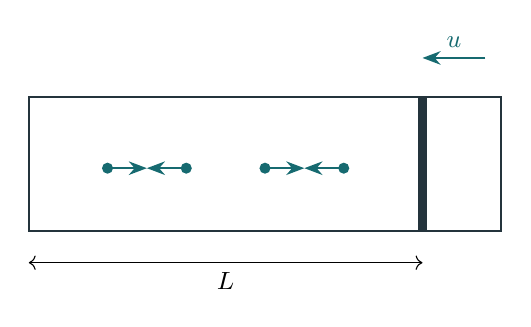
\begin{tikzpicture}[x=1cm,y=1cm,font=\small,every node/.append style={align=center}]\draw[object] (0,0) rectangle(6,1.7);\draw[object,line width=3pt] (5,0)--(5,1.7);\foreach \x/\d in {1/1,2/-1,3/1,4/-1}{\fill[accent] (\x,.8) circle(2pt);\draw[motion] (\x,.8)--(\x+.5*\d,.8);}\draw[motion] (5.8,2.2)--(5,2.2) node[midway,above]{$u$};\draw[<->] (0,-.4)--(5,-.4) node[midway,below]{$L$};\end{tikzpicture}\figcaption{图 热3.4　小球只作一维运动，右活塞缓慢内推。}\end{minipage}\end{center}

\Needspace{8\baselineskip}\subsection*{解答}

取管长$L$，活塞内推速率$u>0$，故$\dot L=-u$。相同球的弹性正碰只交换速度，可以追踪某一速率的“携带者”。
\begin{center}\begin{minipage}{0.96\linewidth}\centering\begin{tikzpicture}[x=1cm,y=1cm,font=\small,every node/.append style={align=center}]\draw[object] (0,0) rectangle(6,1.7);\draw[object,line width=3pt] (5,0)--(5,1.7);\foreach \x/\d in {1/1,2/-1,3/1,4/-1}{\fill[accent] (\x,.8) circle(2pt);\draw[motion] (\x,.8)--(\x+.5*\d,.8);}\draw[motion] (5.8,2.2)--(5,2.2) node[midway,above]{$u$};\draw[<->] (0,-.4)--(5,-.4) node[midway,below]{$L$};\node[above] at (2.5,2.2){$v\to v+2u$，两次碰壁间隔$2L/v$};\end{tikzpicture}\figcaption{解图 热3.4A　追踪速率携带者；单次增速与碰撞频率共同决定平均增能。}\end{minipage}\end{center}
取解图热3.4A向右为正，右端活塞速度为$-u$，迎面入射小球速度为$+v$。
转到活塞参考系，入射速度为$v-(-u)=v+u$。弹性反射使相对速度反号，回到实验室系后
\[
v_{\rm out}=-(v+u)+(-u)=-v-2u.
\]
出射方向向左，速度分量为 $-v-2u$，速率从 $v$ 增至 $v+2u$。
单次碰撞增加的动能为
\[
\Delta\varepsilon=\frac m2[(v+2u)^2-v^2]=2muv+2mu^2\simeq2muv.
\]
最后一步保留$u/v$的一阶项。小球到左壁反射后再回到活塞，在$u\ll v$下往返时间约为$2L/v$；
这一周期中活塞的位移与$L$之比为$2u/v\ll1$，可把碰撞序列视为慢变过程。于是
\[\dot v\simeq\frac{2u}{2L/v}=\frac{uv}{L},\qquad L\dd v+v\dd L=0.\]
对单球动能$\varepsilon=mv^2/2$，乘以$mv$得
\[L\dd\varepsilon+2\varepsilon\dd L=0.\]
各速度携带者遵循同一缩放，平均后
\[L\dd\langle\varepsilon\rangle+2\langle\varepsilon\rangle\dd L=0.\]
以$\langle\varepsilon\rangle=kT/2$定义温度，且$V=SL$，所以
\[\frac{\dd T}{T}+2\frac{\dd V}{V}=0,
\quad\ln\frac{T}{T_0}+2\ln\frac{V}{V_0}=0.\]
\result{TV^2=T_0V_0^2.}
\textbf{一维气体的内能与绝热关系。} 一维只有一个平动自由度，$U=NkT/2$。端面压力由碰撞频率与冲量相乘，$p=Nm\langle v^2\rangle/V=NkT/V$。绝热时
\[\dd U=-p\dd V\ \Rightarrow\ \frac12Nk\dd T=-\frac{NkT}{V}\dd V,\]
分离变量积分得到上面的$TV^2=T_0V_0^2$。一维$C_V=R/2,C_p=C_V+R=3R/2$，故$\gamma=3$。慢压缩时，活塞速率远小于小球的典型速率，相邻两次碰撞之间的容器长度只改变一小段，因而可以用上面的连续微分式描述平均能量变化。
\subsubsection*{把单次反射、碰撞间隔与连续压缩连起来}
解图热3.4B分别在实验室系和活塞系标出速度，
向右为同一正方向。实验室系活塞速度是$-u$，
入射速度$+v$；活塞系入射为$+(v+u)$，反射后为$-(v+u)$。
加回活塞的$-u$，才得到实验室系的$-(v+2u)$。
所增的是速率$2u$，速度分量本身则从正变负。

\begin{center}\begin{minipage}{0.96\linewidth}\centering
\begin{tikzpicture}[x=1cm,y=1cm,font=\small]
\begin{scope}
\draw[object,line width=2pt] (3,0)--(3,2);
\draw[motion] (.3,1.4)--(2.4,1.4) node[midway,above] {$+v$};
\draw[motion] (2.4,.5)--(.3,.5) node[midway,below] {$-v-2u$};
\draw[motion] (3.4,2.3)--(2.6,2.3) node[midway,above] {$-u$};
\node[above] at (1.4,3) {实验室系};
\end{scope}
\begin{scope}[xshift=6cm]
\draw[object,line width=2pt] (3,0)--(3,2);
\draw[motion] (.3,1.4)--(2.4,1.4) node[midway,above] {$+(v+u)$};
\draw[motion] (2.4,.5)--(.3,.5) node[midway,below] {$-(v+u)$};
\node[above] at (3,2.3) {活塞静止};
\node[above] at (1.4,3) {活塞系};
\end{scope}
\end{tikzpicture}
\figcaption{解图 热3.4B　两参考系使用同一正方向；在活塞系作弹性反射，再变回实验室系。}
\end{minipage}\end{center}
单次增能$2muv+2mu^2$中的二次项与一次项之比为$u/v$。
往返时间$2L/v$内，活塞相对位移约$2uL/v$，
与 $L$ 之比为 $2u/v$。慢推使同一次往返的容器长度改变量和速率改变量都很小，分别控制碰撞间隔与增能的近似。

相同小球的弹性正碰只交换速度；
将速度标签跟随碰撞继续传递，等效于标签轨迹穿过彼此。
连续追踪这个速率时，球间每发生一次交换，就转到携带同一速率的另一球。
慢变极限给
\[
L\dd v+v\dd L=0,\qquad
\dd(Lv)=0,\qquad
v=v_0\frac{L_0}{L}.
\]
平方后逐个携带者都有
\[
\varepsilon L^2=\varepsilon_0L_0^2,\qquad
L\dd\varepsilon+2\varepsilon\dd L=0.
\]
容器长度L对所有标签相同，因此对这条关系平均可得到
$\langle\varepsilon\rangle L^2$恒定，
再由温度定义得到$TL^2$恒定。
截面积保持S不变，$V/V_0=L/L_0$，才转为$TV^2$恒定。

\subsubsection*{从端面冲量独立求压强和热容量}
在同一慢变、随机相位的近似下，
一个速率v的球撞固定端面的频率为$v/(2L)$，
每次法向冲量$2mv$，因此平均力为$mv^2/L$。
对N个球求和并除截面积S，
\[
p=\frac{Nm\langle v^2\rangle}{SL}
=\frac{2N\langle\varepsilon\rangle}{V}
=\frac{NkT}{V}.
\]
系统总能量$U=N\langle\varepsilon\rangle=NkT/2$，
绝热内推的外界功使$\dd U=-p\dd V$，故
\[
V\dd T+2T\dd V=0,\qquad
\ln(T/T_0)+2\ln(V/V_0)=0.
\]
由$pV=NkT$还可得
\[
pV^3=p_0V_0^3,\qquad
T/T_0=(V_0/V)^2,\qquad p/p_0=(V_0/V)^3.
\]
体积减半时，上式给温度为4倍、压强为8倍。

一般能量均分模型中，设有效二次项数$i=t+r+2s$，
t为平动项数，r为转动项数，s个已激发振动模式各含动能与势能两项。
有
\[
C_V=\frac i2R,\qquad C_p=\frac{i+2}{2}R,\qquad
\gamma=\frac{i+2}{i}.
\]
本题为只作一维平动的质点，$t=1,r=s=0$，
所以$i=1,\gamma=3$，代$TV^{\gamma-1}$仍给$TV^2$。
三维单原子气体有三个平动项，$t=3$，由同一热容量关系得到 $\gamma=5/3$。

温度由平均动能定义。相同质点的一维弹性碰撞交换已有的速度，保留速率分布。慢推时，各速度标签按同一因子缩放，因而任一给定初始分布都可用该缩放关系求平均能量。$u/v\ll1$ 适用于贡献主要动能的典型速率。若活塞速度可与球速相比，改用实际的相遇时刻和反射速度逐次计算。


\Needspace{18\baselineskip}

\pdfbookmark[2]{第 5 题 光子气压强、能量密度与绝热方程}{q5}

\section*{第 5 题\quad 光子气压强、能量密度与绝热方程}

空腔中已经建立热平衡的热辐射可作为光子气处理，壁面对光子的反射用于计算动量通量。设辐射能量密度为$u$，求压强$p$；论证宏观热平衡辐射的$u$只由温度$T$决定；证明$p\propto T^4$，并导出准静态绝热过程的$p-V$关系。这里讨论热平衡辐射，光子数无独立守恒约束。

\begin{center}\begin{minipage}{0.96\linewidth}\centering\begin{tikzpicture}[x=1cm,y=1cm,font=\small]
\draw[object] (0,0) rectangle (5,4.2);
\node at (1.7,2.6) {热平衡辐射：$u,T$};
\draw[motion] (2,.2)--(5,2) node[pos=.28,below right] {入射};
\draw[motion] (5,2)--(2,3.8) node[pos=.35,above right] {反射};
\draw[guide] (3.5,2)--(5,2);
\draw (4.3,2) arc[start angle=180,end angle=149.036,radius=.7];
\node at (4.05,2.22) {$\theta$};
\draw[force] (5,2)--(6.2,2);
\node[above,align=center] at (6.15,2.45) {壁所受冲量\\$2\epsilon\cos\theta/c$};
\node[below right] at (5.03,1.94) {R};
\end{tikzpicture}\figcaption{图 热3.5　光子在壁面反射，法向动量发生改变。}\end{minipage}\end{center}

\Needspace{8\baselineskip}\subsection*{解答}

\textbf{辐射压。} 光子能量$\epsilon=h\nu$、动量大小$\epsilon/c$。取壁面法向$x$，入射方向余弦$\cos\theta>0$；反射传递$2(\epsilon/c)\cos\theta$。各向同性时方向的能量密度为$u\dd\Omega/(4\pi)$，入射能流再乘$c\cos\theta$。故
\[p=\frac{2u}{4\pi}\int_{\rm hemisphere}\cos^2\theta\dd\Omega
=\frac{u}{2\pi}\,2\pi\int_0^{\pi/2}\cos^2\theta\sin\theta\dd\theta=\frac u3.\]
\begin{center}\begin{minipage}{0.96\linewidth}\centering\begin{tikzpicture}[x=1cm,y=1cm,font=\small]
\draw[object] (0,0) rectangle (5,4.2);
\node at (1.7,2.6) {热平衡辐射：$u,T$};
\draw[motion] (2,.2)--(5,2) node[pos=.28,below right] {入射};
\draw[motion] (5,2)--(2,3.8) node[pos=.35,above right] {反射};
\draw[guide] (3.5,2)--(5,2);
\draw (4.3,2) arc[start angle=180,end angle=149.036,radius=.7];
\node at (4.05,2.22) {$\theta$};
\draw[force] (5,2)--(6.2,2);
\node[above,align=center] at (6.15,2.45) {壁所受冲量\\$2\epsilon\cos\theta/c$};
\node[below right] at (5.03,1.94) {R};
\end{tikzpicture}\figcaption{解图 热3.5A　入射能流与反射冲量分别带一个方向余弦，角积分给$1/3$。}\end{minipage}\end{center}
解图热3.5A的反射几何中，一个$\cos\theta$来自每次碰壁的法向动量变化，另一个来自单位时间能撞到壁面的入射能流；两者相乘才得到压强积分中的$\cos^2\theta$。解图热3.5B则比较同温两腔穿过小孔的双向通量，两腔各自已热化，同温使两向能流相等，从而确定共同的 $u(T)$。

各频率的压强贡献为$p_\nu=u_\nu/3$，再求和得到总压强；光子的动量关系不需要静止质量。

\textbf{能量密度与温度。} 让两个同温的宏观空腔经很小的孔交换热平衡辐射。按解图热3.5B的箭头，两边射入对侧的能量通量分别是 $cu_1/4$ 和 $cu_2/4$。热平衡时它们相等，故 $u_1=u_2$；在这个各向同性的空腔模型中，平衡能量密度只由共同温度确定，记作 $u(T)$。
\begin{center}\begin{minipage}{0.96\linewidth}\centering\begin{tikzpicture}[x=1cm,y=1cm,font=\small]
\draw[object,fill=accent!5] (0,0) rectangle (6,2.5);
\draw[object] (3,0)--(3,1.05) (3,1.45)--(3,2.5);
\node[align=center] at (1.15,1.25) {空腔A\\$T,u_A$};
\node[align=center] at (4.85,1.25) {空腔B\\$T,u_B$};
\draw[motion] (2.1,1.35)--(3.9,1.35);
\draw[force] (3.9,1.15)--(2.1,1.15);
\node[text=accent] at (1.5,2.05) {$cu_A/4$};
\node[text=warm] at (4.5,.4) {$cu_B/4$};
\node[above] at (3,2.75) {同温辐射交换};
\end{tikzpicture}\figcaption{解图 热3.5B　热平衡要求穿孔的两向能量通量相等，宏观辐射能量密度一致。}\end{minipage}\end{center}
同温论证用的是已热化的两腔。若用带活塞的循环表述这一论证，循环末应恢复两腔及活塞状态。理想镜壁只改变光线方向，镜面腔内的未热化光束可以保留由初态决定的能量密度。

\textbf{求温度律。} $U=u(T)V$，可逆微分$\dd U=T\dd S-p\dd V$。令$F=U-TS$，则$\dd F=-S\dd T-p\dd V$，混合偏导相等给
\[\left(\frac{\partial S}{\partial V}\right)_T=\left(\frac{\partial p}{\partial T}\right)_V,\quad
\left(\frac{\partial U}{\partial V}\right)_T=T\left(\frac{\partial p}{\partial T}\right)_V-p.\]
代入$p=u/3$与$U=uV$：
\[u=\frac T3\frac{\dd u}{\dd T}-\frac u3,
\quad\frac{\dd u}{u}=4\frac{\dd T}{T}.
\]
因此 $u=a_rT^4$，$p=a_rT^4/3$。比例常数 $a_r$ 由辐射的微观统计确定，或由一个参考态的 $u/T^4$ 得到。

\textbf{准静态绝热。} $\dd U=-p\dd V$，而$U=3pV$，
\[3V\dd p+3p\dd V=-p\dd V,
\quad\frac{\dd p}{p}=-\frac43\frac{\dd V}{V}.\]
\result{pV^{4/3}=\text{常量},\qquad TV^{1/3}=\text{常量}.}
同一曲线也由 $S=4a_rVT^3/3$ 恒定给出。$4/3$ 是绝热压强曲线的指数。热平衡光子气的压强由温度确定，定压过程也等温，通常用升温定义的 $C_p$ 在这里没有独立定义。
\subsubsection*{把半球通量、频率分量与总能量密度分清}
解图热3.5A的入射点就在反射壁上，反射前后切向动量相同，
法向动量反号。以指向壁外为正，壁所受冲量为正，
而光子所受法向冲量为负，两者大小相等。
频率落在一个小区间内的光子，能量密度记为$u_\nu\dd\nu$；
单光子能量为$h\nu$，动量大小为$h\nu/c$，
故同一角积分给
\[
p_\nu\dd\nu=\frac13u_\nu\dd\nu,\qquad
p=\int_0^\infty p_\nu\dd\nu
=\frac13\int_0^\infty u_\nu\dd\nu=\frac u3.
\]
反射计算直接用光子动量 $h\nu/c$。这里的 $u$ 合计腔内所有传播方向和频率。讨论定向光束时，可分别记入射能量密度、反射能量密度和两者之和。

解图热3.5B中两支箭头都穿过隔板的小孔。
一次穿孔的能量没有反射冲量因子，其单位面积单向能流为
\[
J_E=\frac{cu}{4\pi}\int_{\rm hemisphere}\cos\theta\dd\Omega
=\frac{cu}{4\pi}\,2\pi\int_0^{\pi/2}\cos\theta\sin\theta\dd\theta
=\frac{cu}{4}.
\]
因此同温两腔的净能流密度为$c(u_A-u_B)/4$。
本题已给出热平衡辐射，且光子数没有独立守恒约束；
宏观热平衡的同温两腔，穿孔净交换为零，所以两腔的能量密度相同。壁与辐射交换能量并参与热化时，腔内能量密度可由平衡温度确定。

\subsubsection*{从自由能逐项推出温度四次方律}
在平衡状态空间以T、V为独立变量，写
\[
S=-\left(\frac{\partial F}{\partial T}\right)_V,\qquad
p=-\left(\frac{\partial F}{\partial V}\right)_T.
\]
对第一式求V偏导，对第二式求T偏导，
利用F的混合偏导交换，便得到前面的麦克斯韦关系。
另一方面，在$\dd T=0$时由$\dd U=T\dd S-p\dd V$得
\[
\left(\frac{\partial U}{\partial V}\right)_T
=T\left(\frac{\partial S}{\partial V}\right)_T-p
=T\left(\frac{\partial p}{\partial T}\right)_V-p.
\]
等温偏导比较的是温度相同而体积略有不同的相邻平衡态。
左边对$U=u(T)V$求导为u，右边的压强导数为$u'(T)/3$，
所以$3u=Tu'-u$，即$Tu'=4u$。取一个非零温度参考态，
\[
\ln\frac{u}{u_0}=4\ln\frac{T}{T_0},\qquad
\frac{u}{u_0}=\left(\frac{T}{T_0}\right)^4,\qquad
\frac{p}{p_0}=\left(\frac{T}{T_0}\right)^4.
\]
常数$a_r=u_0/T_0^4$的单位为$\mathrm{J\,m^{-3}\,K^{-4}}$。
其具体数值需要辐射的微观统计，现有热力学关系只确定幂次。

\subsubsection*{光子气的熵、绝热线和等温供热}
代$U=a_rVT^4$和$p=a_rT^4/3$，有
\[
\dd U=4a_rVT^3\dd T+a_rT^4\dd V,
\qquad
\dd S=\frac{\dd U+p\dd V}{T}
=4a_rVT^2\dd T+\frac43a_rT^3\dd V.
\]
右边正是$\dd(4a_rVT^3/3)$，故
\[
S=\frac43a_rVT^3+S_0.
\]
在零温辐射熵取零的宏观模型中，$S_0=0$。
可逆绝热保持S不变，遂有$VT^3$不变，
从而$TV^{1/3}$、$pV^{4/3}$都不变；
总能量$U=a_rVT^4$则满足$UV^{1/3}$不变。
体积增加时温度降低，内能减少量转为壁面对外作功，符号与$\dd U=-p\dd V$一致。
若改为等温膨胀，辐射能量密度不变但总能量随体积增加：
\[
\Delta U=u\Delta V,\qquad W=\frac u3\Delta V,\qquad
Q=\Delta U+W=\frac43u\Delta V.
\]
定容时总热容量为$4a_rVT^3$。
光子气的压强由温度唯一决定，定压过程同时是等温过程。此时供热可以随体积变化，温升恒为零。通常以非零温升定义的定压热容量在这里没有定义，绝热指数$4/3$由熵随$V,T$的变化确定。


\Needspace{18\baselineskip}

\pdfbookmark[2]{第 6 题 混合理想气体分子相对速率}{q6}

\section*{第 6 题\quad 混合理想气体分子相对速率}

混合理想气体处于温度$T$的平衡态，任取两个质量$m_1,m_2$的分子，其速度相互独立，$\bm u=\bm v_1-\bm v_2$。求相对速率的方均根值$\sqrt{\langle u^2\rangle}$和平均值$\langle u\rangle$。要求给出相对速度分布的推导，并讨论$m_1=m_2$及$m_2\gg m_1$。

\begin{center}\begin{minipage}{0.96\linewidth}\centering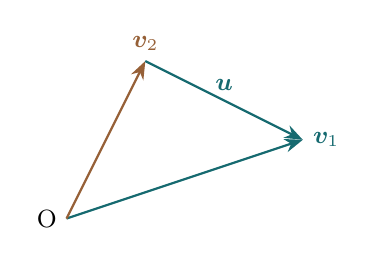
\begin{tikzpicture}[x=1cm,y=1cm,font=\small,every node/.append style={align=center}]\draw[motion] (0,0)--(3,1) node[right]{$\bm v_1$};\draw[force] (0,0)--(1,2) node[above]{$\bm v_2$};\draw[motion] (1,2)--(3,1) node[midway,above]{$\bm u$};\node[left] at (0,0){O};\end{tikzpicture}\figcaption{图 热3.6　相对速度为两个速度矢量之差。}\end{minipage}\end{center}

\Needspace{8\baselineskip}\subsection*{解答}

解图热3.6A把两分子的速度分成质心速度与相对速度。解图热3.6B用同质量情形比较速率分布，下面的变量变换说明曲线宽度怎样改变。

设$s=m_1+m_2$，约化质量$\mu_r=m_1m_2/s$，质心速度$\bm V=(m_1\bm v_1+m_2\bm v_2)/s$。逆变换为
\[\bm v_1=\bm V+\frac{m_2}{s}\bm u,\qquad\bm v_2=\bm V-\frac{m_1}{s}\bm u.\]
\begin{center}\begin{minipage}{0.96\linewidth}\centering\begin{tikzpicture}[x=1.3cm,y=1.3cm,font=\small]
\draw[motion] (0,0)--(3,1) node[right] {$\bm v_1$};
\draw[force] (0,0)--(1,2) node[above] {$\bm v_2$};
\draw[motion] (1,2)--(3,1) node[pos=.7,above right] {$\bm u$};
\draw[object,->] (0,0)--(1.66667,1.66667)
 node[pos=.6,below right] {$\bm V$};
\fill (1.66667,1.66667) circle (1.2pt);
\node[left] at (0,0) {O};
\node[below,align=center] at (1.5,-.5)
 {$m_1:m_2=1:2$（几何示例）\\
 $\bm V=(m_1\bm v_1+m_2\bm v_2)/(m_1+m_2)$};
\end{tikzpicture}\figcaption{解图 热3.6A　相对运动与质心运动分开，联合分布中的动能可分解为两项。}\end{minipage}\end{center}
\textbf{先求方均根。} 两分子速度独立、均值为零，故
\[\langle\bm v_1\cdot\bm v_2\rangle=0,\qquad
\langle u^2\rangle=\langle v_1^2\rangle+\langle v_2^2\rangle
=3kT\left(\frac1{m_1}+\frac1{m_2}\right)=\frac{3kT}{\mu_r}.\]
\textbf{完整分布变换。} 将逆变换代入动能，先分别保留三类项：
\[\begin{aligned}
\frac12m_1v_1^2+\frac12m_2v_2^2
&=\frac{m_1+m_2}{2}V^2
+\left(\frac{m_1m_2}{s}-\frac{m_2m_1}{s}\right)\bm V\cdot\bm u\\
&\quad+\frac12\left(\frac{m_1m_2^2+m_2m_1^2}{s^2}\right)u^2\\
&=\frac12sV^2+\frac12\mu_ru^2.
\end{aligned}\]
图中的质心运动与相对运动由此分开，交叉项恰好消去；相对运动的系数是约化质量。
为说明六维体积元，按$u_x,u_y,u_z,V_x,V_y,V_z$排列，其正变换矩阵为
\[J'=\frac{\partial(\bm u,\bm V)}{\partial(\bm v_1,\bm v_2)}=
\begin{pmatrix}
1&0&0&-1&0&0\\0&1&0&0&-1&0\\0&0&1&0&0&-1\\
 m_1/s&0&0&m_2/s&0&0\\0&m_1/s&0&0&m_2/s&0\\0&0&m_1/s&0&0&m_2/s
\end{pmatrix}.\]
后面三行分别减去$m_1/s$倍的前面对应行，右下块变为单位矩阵，上三角块行列式为1。因此$|\det J'|=1$，逆变换的绝对行列式也为1，$\dd^3v_1\dd^3v_2=\dd^3u\dd^3V$。

两个麦克斯韦速度密度的乘积为
\[\left(\frac{m_1m_2}{(2\pi kT)^2}\right)^{3/2}
\exp\left[-\frac{m_1v_1^2+m_2v_2^2}{2kT}\right].\]
利用$m_1m_2=s\mu_r$和动能分解，联合概率密度分解成
\[\left(\frac{s}{2\pi kT}\right)^{3/2}e^{-sV^2/(2kT)}
\left(\frac{\mu_r}{2\pi kT}\right)^{3/2}e^{-\mu_ru^2/(2kT)}.\]
对所有$\bm V$积分，第一因子积分为1；相对速度密度及相对速率密度分别为
\[g_u(\bm u)=\left(\frac{\mu_r}{2\pi kT}\right)^{3/2}e^{-\mu_ru^2/(2kT)},\]
\[f_u(u)=4\pi u^2\left(\frac{\mu_r}{2\pi kT}\right)^{3/2}e^{-\mu_ru^2/(2kT)},\qquad u\ge0.\]
\begin{center}\begin{minipage}{0.96\linewidth}\centering\begin{tikzpicture}[x=1.1cm,y=4cm,font=\small]
\draw[axis] (0,0)--(6.5,0) node[right] {$w$};
\draw[axis] (0,0)--(0,.85) node[above] {无量纲速率密度};
\draw[traj,domain=0:6,samples=120]
 plot (\x,{sqrt(2/pi)*\x*\x*exp(-\x*\x/2)});
\draw[warm,thick,domain=0:6,samples=120]
 plot (\x,{\x*\x*exp(-\x*\x/4)/(2*sqrt(pi))});
\draw[guide] (1.41421,0)--(1.41421,.58705);
\draw[guide] (2,0)--(2,.41511);
\node[below] at (1.41421,0) {$\sqrt2$};
\node[below] at (2,0) {$2$};
\node[below] at (5,-.12) {$w=u/\sqrt{kT/m}$};
\draw[traj] (3.2,.72)--(3.8,.72);
\node[right] at (3.9,.72) {单分子};
\draw[warm,thick] (3.2,.61)--(3.8,.61);
\node[right] at (3.9,.61) {相对速率};
\end{tikzpicture}\figcaption{解图 热3.6B　同质量分子的示例：相对速率分布更宽，三个代表速率均增为$\sqrt2$倍。}\end{minipage}\end{center}
设$a=\mu_r/(2kT)$，用$\int_0^\infty u^3e^{-au^2}\dd u=1/(2a^2)$求平均，得到
\result{\langle u\rangle=\sqrt{\frac{8kT}{\pi\mu_r}},\qquad
\sqrt{\langle u^2\rangle}=\sqrt{\frac{3kT}{\mu_r}}.}
若$m_1=m_2=m$，$\mu_r=m/2$，两量均为单分子对应量的$\sqrt2$倍；若$m_2\gg m_1$，$\mu_r\simeq m_1$，重分子可近似当作静止靶。还可写
\[\langle u\rangle=\sqrt{\bar v_1^2+\bar v_2^2},\qquad
\langle u^2\rangle=\langle v_1^2\rangle+\langle v_2^2\rangle.\]
第一式使用两个组分独立、零漂移且各向同性的麦克斯韦速度分布。$\langle\bm u\rangle=0$来自各方向的矢量平均相消，速率的平均$\langle u\rangle$则按非负的矢量长度计算。
少量杂质粒子与大量背景气体达到热平衡后，杂质也服从由自身质量和共同温度确定的麦克斯韦分布。
这里的平均可由反复制备的平衡样本取得；在满足充分取样条件时，也可沿单个杂质的长时间运动取样。
各组分的样本数可由重复取样积累，每次配对取自平衡分布，且两次抽取相互独立。
\subsubsection*{速度分量的正、逆变换与雅可比}
解图热3.6A中，连接$\bm v_2$与$\bm v_1$的箭头端点，方向从前者指向后者，便得到相对速度。图中取$m_1:m_2=1:2$，质心速度的端点在连线上，离较重分子的速度端点更近。下面的变换把图中的权重写成任意正质量的比。
同一方向的正、逆变换矩阵为
\[
\begin{pmatrix}u_x\\V_x\end{pmatrix}
=\begin{pmatrix}1&-1\\m_1/s&m_2/s\end{pmatrix}
\begin{pmatrix}v_{1x}\\v_{2x}\end{pmatrix},\qquad
\begin{pmatrix}v_{1x}\\v_{2x}\end{pmatrix}
=\begin{pmatrix}m_2/s&1\\-m_1/s&1\end{pmatrix}
\begin{pmatrix}u_x\\V_x\end{pmatrix}.
\]
两行列式都等于$(m_1+m_2)/s=1$。
三个方向各作同样变换，体积元的绝对因子仍为1；
所得体积元因子与六阶矩阵的行变换一致。
若改变变量排列顺序，行列式可能变号，但概率积分使用的是绝对值。

\subsubsection*{用一维卷积独立得到相对速度分布}
两个独立速度分量的差服从卷积所得的分布。先沿$x$方向计算。
令$a_1=m_1/(2kT)$、$a_2=m_2/(2kT)$。
在$x$方向，两个独立速度分量的密度为
$g_i(v)=\sqrt{a_i/\pi}\exp(-a_iv^2)$。
要求差值为$u_x$，可令$v_{1x}=v$、$v_{2x}=v-u_x$，
对所有v相加，得
\[
g_{u_x}(u_x)=\frac{\sqrt{a_1a_2}}{\pi}
\int_{-\infty}^\infty
\exp[-a_1v^2-a_2(v-u_x)^2]\dd v.
\]
配方时保留常数项：
\[
a_1v^2+a_2(v-u_x)^2
=(a_1+a_2)\left(v-\frac{a_2u_x}{a_1+a_2}\right)^2
+\frac{a_1a_2}{a_1+a_2}u_x^2.
\]
其中平移不改变全实轴高斯积分，故
\[
\begin{aligned}
g_{u_x}(u_x)
&=\frac{\sqrt{a_1a_2}}{\pi}
\sqrt{\frac{\pi}{a_1+a_2}}
\exp\left[-\frac{a_1a_2}{a_1+a_2}u_x^2\right]\\
&=\sqrt{\frac{\mu_r}{2\pi kT}}
\exp\left[-\frac{\mu_ru_x^2}{2kT}\right].
\end{aligned}
\]
三个方向的差仍独立，三式相乘就得到$g_u(\bm u)$。
它是每单位速度空间体积的密度；
速率在$u$到$u+\dd u$之间对应半径u的薄球壳，
还须乘球壳体积$4\pi u^2\dd u$。
因此$g_u$在零矢量处最大，但速率密度$f_u$在$u=0$处为零，
两处峰值分别对应三维速度密度和径向速率密度。

\subsubsection*{归一化、平均速率和方均根逐项积分}
记$a=\mu_r/(2kT)$、$A=4\pi(a/\pi)^{3/2}$，则$f_u(u)=Au^2e^{-au^2}$。
变量代换$t=au^2$给
\[
I_j(a)=\int_0^\infty u^je^{-au^2}\dd u
=\frac12a^{-(j+1)/2}
\Gamma\left(\frac{j+1}{2}\right).
\]
分别用$\Gamma(3/2)=\sqrt\pi/2$、
$\Gamma(2)=1$、$\Gamma(5/2)=3\sqrt\pi/4$，有
\[
I_2=\frac{\sqrt\pi}{4a^{3/2}},\qquad
I_3=\frac1{2a^2},\qquad
I_4=\frac{3\sqrt\pi}{8a^{5/2}}.
\]
先算$AI_2=1$，确认球壳密度确已归一化，
再算
\[
\langle u\rangle=AI_3=\frac{2}{\sqrt{\pi a}}
=\sqrt{\frac{8kT}{\pi\mu_r}},\qquad
\langle u^2\rangle=AI_4=\frac3{2a}=\frac{3kT}{\mu_r}.
\]
二阶矩也可直接展开速度差的平方。求一阶矩时，上式使用了薄球壳上的完整概率密度。
由$f_u'(u)=2Au e^{-au^2}(1-au^2)$得非零峰
$u_p=1/\sqrt a=\sqrt{2kT/\mu_r}$，且
\[
u_p<\langle u\rangle<\sqrt{\langle u^2\rangle},\qquad
\frac{\langle u\rangle}{u_p}=\frac2{\sqrt\pi},\quad
\frac{u_{\rm rms}}{u_p}=\sqrt{\frac32}.
\]
解图热3.6B以$w=u/\sqrt{kT/m}$画同质量示例。
单分子无量纲速率密度为$\sqrt{2/\pi}\,w^2e^{-w^2/2}$，
相对速率密度为$w^2e^{-w^2/4}/(2\sqrt\pi)$。
它们各自面积为1，峰分别在$\sqrt2$与2，
较宽的相对速率曲线也相应较低；
三个代表速率同时乘$\sqrt2$。相对速率的横向尺度增为$\sqrt2$倍，纵向密度相应除以$\sqrt2$，以保持总概率为1。

\subsubsection*{同温、独立抽样与碰撞抽样各控制什么}
若两组分各自是无漂移的麦克斯韦速度，但温度分别为$T_1,T_2$，
独立性仍给每个相对分量的方差
\[
\sigma_u^2=\frac{kT_1}{m_1}+\frac{kT_2}{m_2},\qquad
\langle u\rangle=\sqrt{\frac8\pi}\sigma_u,\qquad
u_{\rm rms}=\sqrt3\,\sigma_u.
\]
于是$\langle u\rangle^2=\bar v_1^2+\bar v_2^2$仍成立；
不同温度下仍可把两个独立、零漂移的各向同性高斯分布卷积。同温时方差可以简写为 $kT/\mu_r$，也可由下式看到质心速度与相对速度为何独立：
\[
\operatorname{Cov}(V_x,u_x)
=\frac{k(T_1-T_2)}{m_1+m_2}.
\]
对联合高斯，协方差为零才使这两个变量独立。
共同漂移速度在相减时抵消；不同漂移则留下非零平均相对矢量，
速率分布不再是这里的零中心麦克斯韦形式。

本题取的是随机分子对。
若改成记录单位时间内真正发生碰撞的分子对，
在碰撞截面不随速率变化的稀薄气体模型中，快分子对被抽中的机会还正比于u，
其归一化分布为$f_{\rm coll}(u)=uf_u(u)/\langle u\rangle$。
所以
\[
\langle u\rangle_{\rm coll}
=\frac{\langle u^2\rangle}{\langle u\rangle}
=\frac{3\pi}{8}\langle u\rangle.
\]
碰撞记录的平均速率因抽样权重而增大。若改取速度相关的分子对，二阶矩还包含 $-2\langle\bm v_1\cdot\bm v_2\rangle$，计算完整分布还需指定两速度的联合密度。
\subsubsection*{质心速度积分与两部分平均动能}
先把每个分子的速度减去质心速度，得到两项内部动能所需的速度：
\[
\bm v_1-\bm V=\frac{m_2}{s}(\bm v_1-\bm v_2)
=\frac{m_2}{s}\bm u,\qquad
\bm v_2-\bm V=-\frac{m_1}{s}\bm u.
\]
所以内部动能的两项分别为
\[
K_{\rm int,1}=\frac{m_1m_2^2}{2s^2}u^2,\qquad
K_{\rm int,2}=\frac{m_2m_1^2}{2s^2}u^2,
\]
相加后
\[
K_{\rm int}=\frac{m_1m_2(m_1+m_2)}{2s^2}u^2
=\frac12\mu_ru^2.
\]
两分子在实验室系的总动能等于质心动能$K_{\rm cm}=sV^2/2$与内部动能$K_{\rm int}$之和。分解后，质心速度的贡献全部归入$K_{\rm cm}$。

边缘分布只保留相对速度，因此要在整个质心速度空间积分。记$b=s/(2kT)$、$a=\mu_r/(2kT)$。
由一维高斯积分
\[
\int_{-\infty}^\infty e^{-bV_x^2}\dd V_x=\sqrt{\frac\pi b}
\]
及三分量乘积，质心因子的全空间积分为
\[
\int_{\mathbb R^3}\left(\frac b\pi\right)^{3/2}
e^{-b(V_x^2+V_y^2+V_z^2)}\dd V_x\dd V_y\dd V_z
=\left(\frac b\pi\right)^{3/2}
\left(\sqrt{\frac\pi b}\right)^3=1.
\]
故联合分布的边缘积分具体为
\[
\begin{aligned}
g_u(\bm u)
&=\int_{\mathbb R^3}
\left(\frac b\pi\right)^{3/2}
\left(\frac a\pi\right)^{3/2}
e^{-bV^2-au^2}\dd^3V\\
&=\left(\frac a\pi\right)^{3/2}e^{-au^2}.
\end{aligned}
\]
积分区域是完整的三维质心速度空间，与固定的$\bm u$无关。
积分把每个固定$\bm u$所对应的全部质心速度计入。在质心速率和方向坐标下，同一积分包含整个球面的方向积分和速率的径向积分。两组分同温使联合密度中的质心项和相对项分离。

质心速度与相对速度分别有三个独立的平动分量，平均能量由各自的二阶矩给出：
\[
\langle V^2\rangle=\frac{3kT}{s},\qquad
\langle K_{\rm cm}\rangle=\frac12s\langle V^2\rangle=\frac32kT,
\]
\[
\langle K_{\rm int}\rangle
=\frac12\mu_r\langle u^2\rangle=\frac32kT,\qquad
\left\langle\frac12m_1v_1^2+\frac12m_2v_2^2\right\rangle=3kT.
\]
在质心和相对速度坐标中，每个平动分量贡献$kT/2$，六项合计$3kT$。相对速率的二阶矩使用约化质量$\mu_r$，对速率积分时，球壳因子来自三维速度空间的径向体积元。



\Needspace{18\baselineskip}

\pdfbookmark[2]{第 7 题 最概然平动能与最概然速率比较}{q7}

\section*{第 7 题\quad 最概然平动能与最概然速率比较}

平衡态理想气体中，分子平动能$E=mv^2/2$。最概然平动能记为$E_p$，与之对应的速率为$v_0$；最概然速率为$v_p$。导出平动能概率密度，求$v_0/v_p$，并说明从速率换到平动能后，概率密度的峰值位置为何改变。

\begin{center}\begin{minipage}{0.96\linewidth}\centering\begin{tikzpicture}[x=1cm,y=1cm,font=\small,every node/.append style={align=center}]\node[draw,align=center] (v) at (0,0){速率$v$\\等宽$\dd v$};\node[draw,align=center] (e) at (4,0){动能$E=mv^2/2$\\等宽$\dd E$};\draw[motion] (v)--(e);\node[below] at (2,-.8){同一概率：$f_v\dd v=f_E\dd E$};\end{tikzpicture}\figcaption{图 热3.7　变量改变后，相同宽度区间对应的分子数不按固定比例换算。}\end{minipage}\end{center}

\Needspace{8\baselineskip}\subsection*{解答}

麦克斯韦速率密度为
\[f_v(v)=4\pi\left(\frac{m}{2\pi kT}\right)^{3/2}v^2e^{-mv^2/(2kT)},\qquad v\ge0.\]
变量变换$E=mv^2/2$给$\dd E=mv\dd v=\sqrt{2mE}\dd v$。同一批分子的概率应相等，$f_E(E)\dd E=f_v(v)\dd v$，故
\[f_E(E)=\frac{f_v(\sqrt{2E/m})}{\sqrt{2mE}}
=\frac{2}{\sqrt\pi}(kT)^{-3/2}\sqrt{E}\,e^{-E/(kT)},\qquad E\ge0.\]
\begin{center}\begin{minipage}{0.96\linewidth}\centering\begin{tikzpicture}[x=1cm,y=4cm,font=\small]
\draw[axis] (0,0)--(4.7,0) node[right] {$w$};
\draw[axis] (0,0)--(0,.78) node[above] {$h_v(w)$};
\draw[traj,domain=0:4.4,samples=110]
 plot (\x,{sqrt(2/pi)*\x*\x*exp(-\x*\x/2)});
\draw[guide] (1.41421,0)--(1.41421,.58705);
\node[below] at (1.41421,0) {$\sqrt2$};
\begin{scope}[xshift=7cm]
\draw[axis] (0,0)--(4.7,0) node[right] {$\varepsilon$};
\draw[axis] (0,0)--(0,.78) node[above] {$h_E(\varepsilon)$};
\draw[traj,domain=0:4.4,samples=150]
 plot (\x,{2*sqrt(\x)*exp(-\x)/sqrt(pi)});
\draw[guide] (.5,0)--(.5,.48394);
\node[below] at (.5,0) {$1/2$};
\end{scope}
\end{tikzpicture}\figcaption{解图 热3.7A　各图分别表示本变量的密度形状，峰值在$v/\sqrt{kT/m}=\sqrt2$和$E/(kT)=1/2$。}\end{minipage}\end{center}
例如在$v$附近取同一小宽度$\Delta v$，它映到能量轴的宽度约为$mv\Delta v$，高速区的能量条更宽。相同粒子概率摊到更宽能量区间后，柱高就更低，这正是密度须除以$mv$的原因。以 $u=E/(kT)$ 对整条概率密度积分，得到总概率：
\[\int_0^\infty f_E(E)\dd E
=\frac2{\sqrt\pi}\int_0^\infty u^{1/2}e^{-u}\dd u=1.\]
令$u=y^2$并分部积分，可具体求出上式中的积分：
\[\int_0^\infty u^{1/2}e^{-u}\dd u
=2\int_0^\infty y^2e^{-y^2}\dd y
=\left[-ye^{-y^2}\right]_0^\infty+\int_0^\infty e^{-y^2}\dd y
=\frac{\sqrt\pi}{2}.\]
解图热3.7A两条分布的纵轴分别计每单位速率和每单位能量的概率。比较同一批粒子时，取各自小区间下的曲线面积。

两图分别按等宽速率区间、等宽能量区间计数；$\dd v/\dd E$不恒定，柱宽改变会移动密度峰。对$E>0$取对数导数，
\[\frac{\dd\ln f_E}{\dd E}=\frac1{2E}-\frac1{kT}=0
\ \Rightarrow\ E_p=\frac{kT}{2}.\]
因$f_E$两端趋零且只有此一正极值，它是极大值。于是
\[v_0=\sqrt{\frac{2E_p}{m}}=\sqrt{\frac{kT}{m}}.\]
另一方面，$\dd\ln f_v/\dd v=2/v-mv/(kT)=0$给$v_p=\sqrt{2kT/m}$，所以
\result{\frac{v_0}{v_p}=\frac1{\sqrt2}.}
$v_p$对应动能$kT$，与$E_p=kT/2$不同；平均动能则是$3kT/2$。概率本身在变换中保持，概率密度的最大位置通常不保持。
\subsubsection*{速率密度峰与能量密度峰}
记$C=2/[\sqrt\pi(kT)^{3/2}]$，
则能量密度的普通导数为
\[
f_E'(E)=C e^{-E/(kT)}
\left(\frac{1}{2\sqrt E}-\frac{\sqrt E}{kT}\right)
=\frac{C e^{-E/(kT)}}{2\sqrt E}
\left(1-\frac{2E}{kT}\right).
\]
对$E>0$，前一因子为正，所以导数在$E<kT/2$时为正，
在$E>kT/2$时为负，唯一峰确为$E_p=kT/2$。
速率密度若写为$Dv^2e^{-av^2}$、$a=m/(2kT)$，
则
\[
f_v'(v)=2Dv e^{-av^2}(1-av^2),
\]
其非零峰为$v_p=1/\sqrt a$，对应能量为$mv_p^2/2=kT$。
速率密度峰比较的是等宽速率区间，能量密度峰比较的是等宽能量区间。解图热3.7B画出等宽速率区间如何映成不同宽度的能量区间。

用无量纲变量$w=v/\sqrt{kT/m}$、$\varepsilon=E/(kT)=w^2/2$，
各自归一化的密度为
\[
h_v(w)=\sqrt{\frac2\pi}\,w^2e^{-w^2/2},\qquad
h_E(\varepsilon)=\frac2{\sqrt\pi}\sqrt\varepsilon\,e^{-\varepsilon}.
\]
解图热3.7A画的正是这两条密度，纵轴也按无量纲区间定义，
各自总面积为1；物理密度分别还带$1/\sqrt{kT/m}$和$1/(kT)$的单位因子。
在相应区间上满足
$h_E(\varepsilon)\dd\varepsilon=h_v(w)\dd w$，
由于$\dd\varepsilon=w\dd w$，故$h_E=h_v/w$。
换变量后，密度的数值和单位都随之改变。相应区间内的曲线面积保持相等。

\begin{center}\begin{minipage}{.96\linewidth}\centering
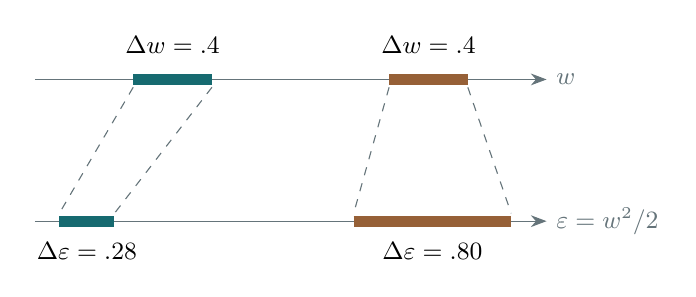
\begin{tikzpicture}[x=2.5cm,y=1cm,font=\small]
\draw[axis] (0,1.8)--(2.6,1.8) node[right] {$w$};
\draw[axis] (0,0)--(2.6,0) node[right] {$\varepsilon=w^2/2$};
\draw[accent,line width=4pt] (.5,1.8)--(.9,1.8);
\draw[warm,line width=4pt] (1.8,1.8)--(2.2,1.8);
\draw[accent,line width=4pt] (.125,0)--(.405,0);
\draw[warm,line width=4pt] (1.62,0)--(2.42,0);
\draw[guide] (.5,1.7)--(.125,.1) (.9,1.7)--(.405,.1);
\draw[guide] (1.8,1.7)--(1.62,.1) (2.2,1.7)--(2.42,.1);
\node[above] at (.7,2) {$\Delta w=.4$};
\node[above] at (2,2) {$\Delta w=.4$};
\node[below] at (.265,-.15) {$\Delta\varepsilon=.28$};
\node[below] at (2.02,-.15) {$\Delta\varepsilon=.80$};
\end{tikzpicture}
\figcaption{解图 热3.7B　两个同宽速率区间变为不同宽能量区间；每个区间内的概率分别保留。}
\end{minipage}\end{center}
图中低速条$[.5,.9]$映成能量条$[.125,.405]$，
高速条$[1.8,2.2]$映成$[1.62,2.42]$。
两条速率区间宽都为.4，能量区间宽却为.28和.80。
每种颜色在两条轴上标出的是同一批粒子，概率在换变量时保持相同。蓝、橙区间之间的概率仍分别由各自所占的曲线面积决定。连续分布在任意单点的概率为零，最概然值指的是指定变量的概率密度最大处。


\Needspace{18\baselineskip}

\pdfbookmark[2]{第 8 题 定容热气球升空后的振动与上升高度}{q8}

\section*{第 8 题\quad 定容热气球升空后的振动与上升高度}

热气球容积恒为$V_B=1.1\,\mathrm{m^3}$，蒙皮质量$m_H=0.187\,\mathrm{kg}$、体积忽略。地面温度20℃，压强$p_1=1.013\times10^5\,\mathrm{Pa}$，空气密度$\rho_1=1.2\,\mathrm{kg/m^3}$。求：开口气球刚好浮起的内部温度；系在地面将内部加热至110℃后释放的初始加速度；在地面扎紧通气口、保持体积和内部温度不变后，在20℃的等温大气中平衡的高度；将气球从该位置竖直拉开10 m再释放后的运动。$M$表示蒙皮与球内气体的总质量。忽略附加质量，最后一问分别讨论有、无阻力，取$g=9.80\,\mathrm{m/s^2}$。

\begin{center}\begin{minipage}{0.96\linewidth}\centering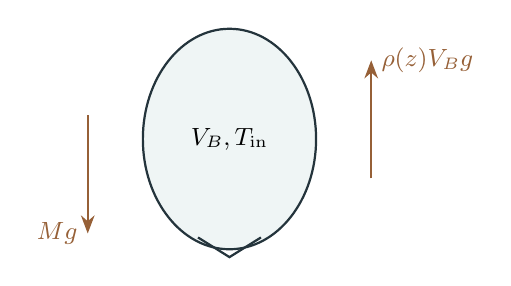
\begin{tikzpicture}[x=1cm,y=1cm,font=\small,every node/.append style={align=center}]\draw[object,fill=accent!7] (0,1) ellipse(1.1 and 1.4);\node at (0,1){$V_B,T_{\rm in}$};\draw[object] (-.4,-.25)--(0,-.5)--(.4,-.25);\draw[force] (1.8,.5)--(1.8,2) node[right]{$\rho(z)V_Bg$};\draw[force] (-1.8,1.3)--(-1.8,-.2) node[left]{$Mg$};\end{tikzpicture}\figcaption{图 热3.8　气球体积固定，浮力随外界密度改变。}\end{minipage}\end{center}

\Needspace{8\baselineskip}\subsection*{解答}

\textbf{地面刚浮起。} 开口时内外压力相同，理想气体密度与绝对温度成反比。令临界内部密度$\rho_2$，
\[\rho_1V_Bg=(\rho_2V_B+m_H)g,\qquad
\rho_2=1.2-\frac{0.187}{1.1}=1.030\,\mathrm{kg/m^3}.\]
\[T_2=\frac{\rho_1}{\rho_2}T_1
=\frac{1.2}{1.03}\,293.15=341.53398\,\mathrm K.\]
故临界温度$t_2=68.38^\circ\mathrm C$。
\begin{center}\begin{minipage}{0.96\linewidth}\centering\begin{tikzpicture}[x=1cm,y=1cm,font=\small,every node/.append style={align=center}]\draw[object,fill=accent!7] (0,1) ellipse(1.1 and 1.4);\node at (0,1){$V_B,T_{\rm in}$};\draw[object] (-.4,-.25)--(0,-.5)--(.4,-.25);\draw[force] (1.8,.5)--(1.8,2) node[right]{$\rho(z)V_Bg$};\draw[force] (-1.8,1.3)--(-1.8,-.2) node[left]{$Mg$};\node[below] at (0,-1){开口时同压；扎口后$M$固定};\end{tikzpicture}\figcaption{解图 热3.8A　地面浮起条件及加速度先由内部密度求空气质量，再加上蒙皮质量。}\end{minipage}\end{center}
解图热3.8A把浮力和总重力作用在同一气球上：浮力用外部空气密度乘排开体积，总重力同时包括蒙皮和内部空气。解图热3.8B以平衡高度为位移零点，曲线在零点的斜率为$-Mg/H_s$，小振动刚度为其绝对值。从地面释放后的最高点由净力的功确定，到该处时速度第一次降为零。

\textbf{加热至110℃。} $T_3=383.15\,\mathrm K$，扎口前装入的空气密度为
\[\rho_3=\rho_1\frac{T_1}{T_3}=0.9181261\,\mathrm{kg/m^3},\quad
M=m_H+\rho_3V_B=1.1969387\,\mathrm{kg}.\]
初始净力为$(1.2\times1.1-M)g=1.2060\,\mathrm N$，因此
\[a_0=g\left(\frac{\rho_1V_B}{M}-1\right)=1.00757\,\mathrm{m/s^2}\simeq1.01\,\mathrm{m/s^2}.\]
\textbf{扎口后的平衡高度。} 封口后球内质量与容积都固定，球内温度由题设保持在封口时的数值。等温大气尺度高度
\[H_s=\frac{RT_1}{\mu g}=\frac{p_1}{\rho_1g}=8613.9456\,\mathrm m,\qquad
\rho(z)=\rho_1e^{-z/H_s}.\]
平衡时$\rho(h)V_B=M$，于是
\result{h=H_s\ln\frac{\rho_1V_B}{M}=842.9999\,\mathrm m\simeq843\,\mathrm m.}
力学平衡高度是净力过零的位置。若从地面无阻力释放，气球到达这里时仍有向上的速度。
\begin{center}\begin{minipage}{0.96\linewidth}\centering\begin{tikzpicture}[x=6cm,y=5cm,font=\small]
\draw[axis] (-.5,0)--(.62,0) node[right] {$\xi=y/H_s$};
\draw[axis] (0,-.5)--(0,.72) node[above] {$F/(Mg)$};
\draw[traj,domain=-.45:.5,samples=100] plot (\x,{exp(-\x)-1});
\draw[warm,thick,domain=-.45:.5] plot (\x,{-\x});
\node[below left] at (0,0) {O};
\draw[traj] (-.43,.66)--(-.3,.66);
\node[right] at (-.28,.66) {$e^{-\xi}-1$};
\draw[warm,thick] (.2,-.13)--(.33,-.13);
\node[right] at (.35,-.13) {$-\xi$};
\end{tikzpicture}\figcaption{解图 热3.8B　合力在坐标原点过零，蓝色为精确曲线，橙色为小振动切线。}\end{minipage}\end{center}
\textbf{平衡附近。} 令$y=z-h$，合力
\[F(y)=Mg(e^{-y/H_s}-1)=-\frac{Mg}{H_s}y+O(y^2/H_s^2).\]
因$10/H_s\simeq1.16\times10^{-3}$，线性化有效。无阻力时
\[\ddot y+\frac g{H_s}y=0,\quad A=10\,\mathrm m,\quad
\mathcal T=2\pi\sqrt{\frac{H_s}{g}}=186.28\,\mathrm s.\]
加入空气阻力后，机械能随运动减少。小振幅下若采用线性阻力，可按系数与临界值的大小分出衰减振荡和单向回落。
\subsubsection*{系统质量与开口、封口条件分别确定}
解图热3.8A的总重力为$(m_H+m_{\rm gas})g$，
浮力为外界空气密度乘固定排开体积再乘g。
刚浮起时$m_{\rm gas}=\rho_2V_B$，
加热至110℃时则为$\rho_3V_B$，两次装入质量不同。
开口、缓慢加热并已稳定的情况下，近似取球内压力等于同高度外压，
用 $\rho=\mu p/(RT)$ 作密度比，温度取开尔文：
\[
T_1=293.15\,\mathrm K,\qquad T_3=383.15\,\mathrm K,\qquad
\frac{\rho_3}{\rho_1}=\frac{293.15}{383.15}.
\]
临界条件先给$\rho_2=1.030\,\mathrm{kg/m^3}$，
代绝对温度求得 $T_2=341.53398\,\mathrm K$。
若$m_H\ge\rho_1V_B$，连内部气体质量趋零也不足以满足严格向上的净力，
不存在有限正温度使此模型自行升空。
本题$m_H/(\rho_1V_B)=0.14167<1$，临界温度可实现于理想模型中。

加速时一同运动的是蒙皮与球内热空气，故惯性质量是两者之和。排开的外界空气质量用于求向上的浮力。
未先将$\rho_3$截断到三位小数时，
\[
\begin{aligned}
m_{\rm gas}&=1.0099387\,\mathrm{kg},\\
M&=m_H+m_{\rm gas}=1.1969387\,\mathrm{kg},\\
\rho_1V_B-M&=0.1230613\,\mathrm{kg},\\
F_{\rm net}(0)&=1.2060009\,\mathrm N,\qquad
a_0=F_{\rm net}(0)/M=1.00757\,\mathrm{m/s^2}.
\end{aligned}
\]
前面算式保留较多小数是为了避免连续截断，按题给数据宜把加速度报为约$1.0\,\mathrm{m/s^2}$。
模型忽略外界流体附加惯性、释放瞬间流动和喷流反作用；
它把释放后的热气球近似作固定总质量的受浮力系统。

\subsubsection*{由大气静力平衡积分密度分布}
等温外界大气在竖直方向满足
\[
\frac{\dd p}{\dd z}=-\rho g,\qquad
\rho=\frac{\mu p}{RT_1},\qquad
\frac{\dd p}{p}=-\frac{\mu g}{RT_1}\dd z.
\]
用地面压强 $p(0)=p_1$ 定积分常数，得
\[
p(z)=p_1e^{-z/H_s},\qquad
\rho(z)=\rho_1e^{-z/H_s},\qquad
H_s=\frac{RT_1}{\mu g}.
\]
用地面状态关系$p_1/\rho_1=RT_1/\mu$，无需另取空气摩尔质量，
就得到$H_s=p_1/(\rho_1g)$。
也可从单分子玻尔兹曼因子$\exp[-m_{\rm air}gz/(kT_1)]$得到同式：
因$\mu=N_Am_{\rm air}$、$R=N_Ak$，
有$kT_1/(m_{\rm air}g)=RT_1/(\mu g)$。
两种证明分别从大气静力平衡和单分子重力分布出发，尺度高度相同。

封口之后，内部质量、体积及题定温度固定，
其密度保持$\rho_3$，内部压力也保持封口时的地面值。
外压和外界密度继续随 $z$ 降低，定容蒙皮承担逐渐增大的内外压差。
净力在全程可写成
\[
F(z)=[\rho_1V_Be^{-z/H_s}-M]g.
\]
它随高度严格下降，因为
$F'(z)=-\rho_1V_Bg e^{-z/H_s}/H_s<0$。
地面净力为正、高处趋于$-Mg$，故恰有一个地面以上平衡点。
取$\bar\rho=M/V_B=1.0881261\,\mathrm{kg/m^3}$，
平衡要求 $\rho(h)=\bar\rho$。蒙皮称重后分摊到排开体积上，使总平均密度比内部热空气密度多 $m_H/V_B$。

\subsubsection*{平衡附近的恢复力、小振动及阻尼条件}
解图热3.8B的横轴是$\xi=y/H_s$，原点就对应$z=h$；
纵轴是$F/(Mg)=e^{-\xi}-1$，切线为$-\xi$。
它在正位移时为负、负位移时为正，直接给稳定性。
逐项展开有
\[
F(y)=Mg\left(-\frac y{H_s}
+\frac{y^2}{2H_s^2}-\frac{y^3}{6H_s^3}+\cdots\right).
\]
展开变量为 $y/H_s$，用它与1的大小关系判断线性化精度。
本题$10/H_s=1.1609\times10^{-3}$，
二次项相对一次项至多约$5.80\times10^{-4}$，
故10 m的小振动可很好地用简谐近似。
牛顿方程除以总质量M给
\[
\omega_0^2=\frac g{H_s}
=\frac{\rho_1g^2}{p_1},\qquad
\mathcal T=\frac{2\pi}{\omega_0}
=2\pi\sqrt{\frac{p_1}{\rho_1g^2}}.
\]
从$y(0)=10\,\mathrm m,\dot y(0)=0$释放，
有$y(t)=10\cos(\omega_0t)\,\mathrm m$；
若从下方拉开，则初相相差$\pi$。
无阻力的精确运动仍受非线性恢复力，简谐式只保留小振幅首阶。
若线性阻力为$-b\dot y$，
\[
M\ddot y+b\dot y+\frac{Mg}{H_s}y=0,\qquad
b_c=2M\sqrt{\frac g{H_s}}.
\]
$0<b<b_c$时振荡衰减；$b=b_c$为临界阻尼，
$b>b_c$为过阻尼，后二者从静止偏离位置释放可不经往复而回到平衡。

\subsubsection*{从地面释放后的上升和转折}
令z从地面量起，无阻力时将上式净力由0积分至z，得
\[
\frac12M\dot z^2
=\rho_1V_BgH_s(1-e^{-z/H_s})-Mgz.
\]
到$z=h$时，前一段净力一直向上，速度并未减为零；
越过h后合力向下，才开始减速。
最高点应使右边重新等于零，取除地面零根以外的正根。
因此h只由力平衡确定，最高点还取决于初始运动状态和耗散。
最后一问是在平衡位置拉开后从静止释放，
它与从地面直接释放是两组不同初始条件。


\Needspace{18\baselineskip}

\pdfbookmark[2]{第 9 题 等温大气重力势能与热运动能量比}{q9}

\section*{第 9 题\quad 等温大气重力势能与热运动能量比}

取地面为重力势能零点，将等温大气视为恒定重力场中的平面气柱。大气以双原子气体为主，平动、转动自由度被激发，振动自由度忽略。估算大气总重力势能与总热运动能量之比，并说明把积分上限取无穷的条件。

\begin{center}\begin{minipage}{0.96\linewidth}\centering\begin{tikzpicture}[x=1.3cm,y=2.8cm,font=\small]
\draw[axis] (0,0)--(5.5,0) node[right] {$x=z/H_i$};
\draw[axis] (0,0)--(0,1.2) node[above] {$n_i/n_{i0}$};
\draw[traj,domain=0:5.1,samples=100] plot (\x,{exp(-\x)});
\node[left] at (0,1) {1};
\draw[guide] (1.5,0)--(1.5,.22313);
\node[below] at (1.5,0) {$z/H_i$};
\end{tikzpicture}\figcaption{图 热3.9　等温大气分子数密度随高度指数衰减。}\end{minipage}\end{center}

\Needspace{8\baselineskip}\subsection*{解答}

对第$i$种分子，定义尺度高度$H_i=kT/(m_ig)$。同温的平面重力场中
\[n_i(z)=n_{i0}e^{-z/H_i},\qquad\dd N_i=n_i(z)S\dd z.\]
\begin{center}\begin{minipage}{0.96\linewidth}\centering\begin{tikzpicture}[x=1.3cm,y=2.8cm,font=\small]
\draw[axis] (0,0)--(5.5,0) node[right] {$x=z/H_i$};
\draw[axis] (0,0)--(0,1.2) node[above] {$n_i/n_{i0}$};
\fill[accent!20,domain=1.4:1.6,samples=20] (1.4,0)--plot (\x,{exp(-\x)})--(1.6,0)--cycle;
\draw[traj,domain=0:5.1,samples=100] plot (\x,{exp(-\x)});
\node[left] at (0,1) {1};
\draw[guide] (1.5,0)--(1.5,.22313);
\node[below] at (1.5,0) {$z/H_i$};
\node[align=center] at (3.6,.68) {窄带：$n_i(z)S\dd z$\\每分子势能$m_igz$};
\end{tikzpicture}\figcaption{解图 热3.9A　分子数与高度权重分别积分；不同组分的尺度高度不同。}\end{minipage}\end{center}
解图热3.9A中沿高度取同样厚度的水平薄层，层内分子数的权重为$e^{-z/H_i}\dd z$；算重力势能时再乘该层的$m_igz$。总分子数用薄层粒子数累加。总势能要在相同的求和中额外乘每层的单分子势能。

以地面势能零点，单分子势能$m_igz$。当$H_i\ll R_\oplus$且高空稀薄尾部可忽略，$g$可近似不变，积分上限可数学上取无穷。则
\[N_i=n_{i0}S\int_0^\infty e^{-z/H_i}\dd z=n_{i0}SH_i,\]
\[E_{g,i}=n_{i0}Sm_ig\int_0^\infty ze^{-z/H_i}\dd z
=n_{i0}Sm_igH_i^2=N_i kT.\]
各组分平均势能同为$kT$，故$E_g=NkT$。以双原子平动、转动的五个自由度估算，$E_{\rm th}=5NkT/2$，
\result{E_g:E_{\rm th}=2:5.}
平面恒重力模型给出指数尾。只要主要积分集中在近地范围内，便可将这个指数积分延伸到无穷。若只取高 $H_c$ 的截断层，
\[\langle E_g\rangle_i=kT\left[1-\frac{H_c/H_i}{e^{H_c/H_i}-1}\right],\]
此式在$H_c\gg H_i$时趋$kT$，在$H_c\ll H_i$时趋$m_igH_c/2$，即薄层近似均匀时的结果。
\subsubsection*{分别计算粒子数与势能积分}
对质量$m_i$的组分，解图热3.9A横轴用$x=z/H_i$，
蓝色曲线为$n_i(z)/n_{i0}=e^{-x}$。
图中窄带表示该高度区间内的分子，取遍各区间再按各自的粒子数加权求平均高度。
先保留有限截断高度$H_c$，记$b=H_c/H_i$，
\[
N_i(H_c)=n_{i0}S\int_0^{H_c}e^{-z/H_i}\dd z
=n_{i0}SH_i(1-e^{-b}).
\]
势能积分多一个z。分部积分得
\[
\begin{aligned}
\int_0^{H_c}ze^{-z/H_i}\dd z
&=[-H_iz e^{-z/H_i}]_0^{H_c}
+H_i\int_0^{H_c}e^{-z/H_i}\dd z\\
&=H_i^2[1-(1+b)e^{-b}].
\end{aligned}
\]
因此
\[
E_{g,i}(H_c)
=n_{i0}Sm_igH_i^2[1-(1+b)e^{-b}],
\]
\[
\frac{E_{g,i}(H_c)}{N_i(H_c)}
=m_igH_i\frac{1-(1+b)e^{-b}}{1-e^{-b}}
=kT\left(1-\frac b{e^b-1}\right).
\]
当b很大时指数尾部消失，分母给总分子数、分子给势能，
相除后m、地面数密度及柱截面积均约去。
质量越大，$H_i$越小；同一高度处势能增加和平均高度降低正好相抵。
当b很小时，$b/(e^b-1)=1-b/2+O(b^2)$，
所以平均势能趋于$m_igH_c/2$，对应近似均匀薄层的平均高度$H_c/2$。

\begin{center}\begin{minipage}{.96\linewidth}\centering
\begin{tikzpicture}[x=1.25cm,y=2.8cm,font=\small]
\draw[axis] (0,0)--(5.7,0) node[right] {$x=z/H_i$};
\draw[axis] (0,0)--(0,1.2) node[above] {归一化贡献};
\draw[traj,domain=0:5.4,samples=100] plot (\x,{exp(-\x)});
\draw[warm,thick,domain=0:5.4,samples=100] plot (\x,{\x*exp(-\x)});
\draw[traj] (2.5,.94)--(3,.94);
\node[right] at (3.1,.94) {粒子数：$e^{-x}$};
\draw[warm,thick] (2.5,.76)--(3,.76);
\node[right] at (3.1,.76) {势能：$xe^{-x}$};
\node[left] at (0,1) {1};
\draw[guide] (1,0)--(1,.36788);
\node[below] at (1,0) {1};
\end{tikzpicture}
\figcaption{解图 热3.9B　高度积分的两种归一化权重各自面积为1；势能贡献还乘高度。}
\end{minipage}\end{center}
解图热3.9B说明：靠近地面的分子最多，但地面势能为零，
每单位高度的势能贡献在$z=H_i$附近最大。
若截去$z>H_c$部分，丢失的粒子数份额为$e^{-b}$，
丢失的势能份额为$(1+b)e^{-b}$。
例如$b=5$时两者约为$0.674\%$与$4.04\%$，
势能的截断误差比粒子数误差多一个因子 $1+b$。
把上限换为无穷时，应能选择覆盖主要贡献的截断尺度，
使各重要组分都有$H_i\ll H_c\ll R_\oplus$；
在所选截断高度处，指数尾的贡献已很小，可把指数式的积分延至无穷远以简化计算。

\subsubsection*{混合气体的能量求和与气柱静力积分}
对所有组分求和时保留各自$N_i$：
\[
E_g=\sum_iN_i kT=NkT,\qquad
E_{\rm th}=\sum_i\frac{f_i}{2}N_i kT,\qquad N=\sum_iN_i.
\]
本题主要双原子分子有三项平动、两项转动，$f_i\simeq5$，
故$E_{\rm th}\simeq5NkT/2$。
$5NkT/2$包括三项平动的$3NkT/2$和两项转动的$NkT$。
若组分的激发自由度不同，比例为
$E_g/E_{\rm th}=2N/\sum_i f_iN_i$，先加总量再作比。

将整个气柱视为一个系统，也可由静力方程把重力势能写成压强积分。
平面气柱满足$\dd p/\dd z=-\rho g$，
在地面取势能零点，有
\[
E_g=S\int_0^\infty z\rho(z)g\dd z
=-S\int_0^\infty z\frac{\dd p}{\dd z}\dd z
=-S[zp(z)]_0^\infty+S\int_0^\infty p(z)\dd z.
\]
指数尾使$zp(z)\to0$，且地面有 $z=0$，
所以$E_g=S\int p\dd z$。
等温理想气体$p(z)=n_{\rm total}(z)kT$，
遂得$E_g=NkT$。
地面为势能零点，指数尾使上端的$zp(z)$趋零，因而式中取的是全气柱的粒子数。如果只积分到有限高度$H$，上端压强非零时还要保留$-SHp(H)$。


\Needspace{18\baselineskip}

\pdfbookmark[2]{第 10 题 大气压强随高度变化与半数分子高度}{q10}

\section*{第 10 题\quad 大气压强随高度变化与半数分子高度}

大气视为摩尔质量$\mu=29.0\times10^{-3}\,\mathrm{kg/mol}$的理想气体，重力加速度$g=9.80\,\mathrm{m/s^2}$恒定，海平面温度$T_0=273.15\,\mathrm K$。由薄层受力平衡导出$\dd p/\dd z$与$p,T$的关系；对等温大气求半数分子位于其下的高度$h$；对满足$Tp^{(1-\gamma)/\gamma}=\text{常量}$的绝热分层，取$\gamma=7/5$，求模型大气层顶高度$H$。

\begin{center}\begin{minipage}{0.96\linewidth}\centering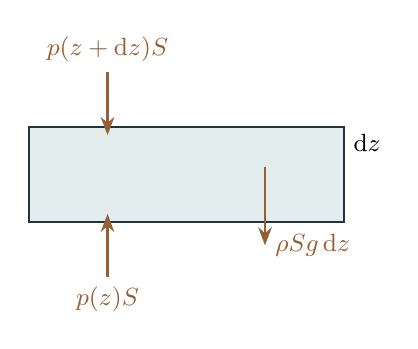
\begin{tikzpicture}[x=1cm,y=1cm,font=\small,every node/.append style={align=center}]\fill[accent!12] (0,0) rectangle(4,1.2);\draw[object] (0,0) rectangle(4,1.2);\draw[force] (1,-.7)--(1,.1) node[pos=0,below]{$p(z)S$};\draw[force] (1,1.9)--(1,1.1) node[pos=0,above]{$p(z+\dd z)S$};\draw[force] (3,.7)--(3,-.3) node[right]{$\rho Sg\dd z$};\node[right] at (4,1){$\dd z$};\end{tikzpicture}\figcaption{图 热3.10　压强差支撑一薄层空气的重量。}\end{minipage}\end{center}

\Needspace{8\baselineskip}\subsection*{解答}

\textbf{薄层平衡。} 取面积$S$、厚$\dd z$的气层，下、上压强差向上的力为$-S\dd p$，重力$\rho Sg\dd z$。静力平衡与理想气体式给
\[\frac{\dd p}{\dd z}=-\rho g=-nmg
=-\frac{\mu gp}{RT(z)}.\]
\begin{center}\begin{minipage}{0.96\linewidth}\centering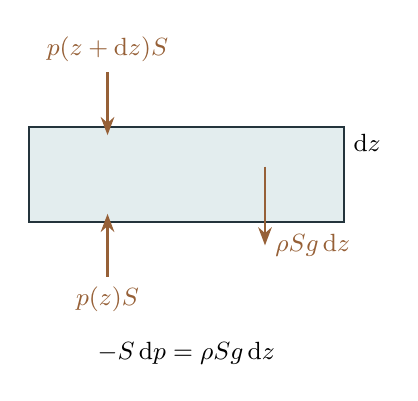
\begin{tikzpicture}[x=1cm,y=1cm,font=\small,every node/.append style={align=center}]\fill[accent!12] (0,0) rectangle(4,1.2);\draw[object] (0,0) rectangle(4,1.2);\draw[force] (1,-.7)--(1,.1) node[pos=0,below]{$p(z)S$};\draw[force] (1,1.9)--(1,1.1) node[pos=0,above]{$p(z+\dd z)S$};\draw[force] (3,.7)--(3,-.3) node[right]{$\rho Sg\dd z$};\node[right] at (4,1){$\dd z$};\node[below] at (2,-1.4){$-S\dd p=\rho Sg\dd z$};\end{tikzpicture}\figcaption{解图 热3.10A　上表面压力向下、下表面向上；压强梯度为负。}\end{minipage}\end{center}
解图热3.10A中的下表面压力向上、上表面压力向下，两者的合力为$-S\dd p$，用来支承薄层重力，故$\dd p/\dd z<0$。解图热3.10B中等温支的指数尾部与绝热支的有限形式顶端不同，后文的中位高度和零温高度须分别从各自曲线计算。

\textbf{等温层的中位高度。} $T=T_0$，积分并取$p(0)=p_0$，
\[p(z)=p_0e^{-z/H_s},\qquad n(z)=n_0e^{-z/H_s},\qquad H_s=\frac{RT_0}{\mu g}.\]
半数分子在$h$下，$\int_0^h n\dd z=\frac12\int_0^\infty n\dd z$，即$1-e^{-h/H_s}=1/2$。
\[h=H_s\ln2=\frac{8.314\times273.15}{0.0290\times9.80}\ln2
=5.539\times10^3\,\mathrm m.\]
\textbf{绝热分层。} 各高度气体满足同一比熵的状态关系
$T/T_0=(p/p_0)^{(\gamma-1)/\gamma}$。先取对数再对$z$求导，
\[
\frac1T\frac{\dd T}{\dd z}
=\frac{\gamma-1}{\gamma}\frac1p\frac{\dd p}{\dd z}
=-\frac{\gamma-1}{\gamma}\frac{\mu g}{RT}.
\]
两边乘$T$，可见温度梯度为常量。用地面条件$T(0)=T_0$积分得到
\[\frac{\dd T}{\dd z}=-\frac{\gamma-1}{\gamma}\frac{\mu g}{R},\qquad
T(z)=T_0\left(1-\frac zH\right),\]
\[H=\frac{\gamma}{\gamma-1}\frac{RT_0}{\mu g}=2.797\times10^4\,\mathrm m.\]
再由状态关系
\[p(z)=p_0(1-z/H)^{\gamma/(\gamma-1)},\quad
n(z)=n_0(1-z/H)^{1/(\gamma-1)},\quad0\le z\le H.\]
直接积分压强方程也可得到压强的幂函数。令$b=(\gamma-1)/\gamma$，有
\[
\frac{\dd p}{\dd z}=-\frac{\mu g}{RT_0}p_0^b p^{1/\gamma},\qquad
\int_{p_0}^{p(z)}p^{-1/\gamma}\dd p
=-\frac{\mu g}{RT_0}p_0^b\int_0^z\dd z.
\]
左边为$[p(z)^b-p_0^b]/b$，所以
\[
\left(\frac{p(z)}{p_0}\right)^b=1-b\frac{\mu g}{RT_0}z=1-\frac zH.
\]
这与先求$T(z)$再代回状态关系的结果相同。除形式顶端的极限外，积分使用$T,p>0$。
\begin{center}\begin{minipage}{0.96\linewidth}\centering\begin{tikzpicture}[x=1.4cm,y=3cm,font=\small]
\draw[axis] (0,0)--(6.1,0) node[right] {$x=z/H_s$};
\draw[axis] (0,0)--(0,1.25) node[above] {$p/p_0$};
\draw[traj,domain=0:5.8,samples=120] plot (\x,{exp(-\x)});
\draw[warm,thick,domain=0:3.5,samples=100] plot (\x,{(1-\x/3.5)^3.5});
\draw[guide] (.693147,0)--(.693147,.5)--(0,.5);
\node[below] at (.693147,0) {$\ln2$};
\node[left] at (0,.5) {$1/2$};
\node[left] at (0,1) {1};
\draw[guide] (3.5,0)--(3.5,.12);
\node[below] at (3.5,0) {$3.5$};
\draw[traj] (2.4,1.08)--(2.9,1.08);
\node[right] at (3,1.08) {等温：指数尾};
\draw[warm,thick] (2.4,.88)--(2.9,.88);
\node[right] at (3,.88) {绝热：$0\le x\le3.5$};
\end{tikzpicture}\figcaption{解图 热3.10B　等温压强指数衰减；绝热模型压强在形式顶端归零。}\end{minipage}\end{center}
\result{h\simeq5.54\,\mathrm{km},\qquad H\simeq28.0\,\mathrm{km}.}
等温气柱在 $h$ 以下容纳半数分子。理想同熵分层的温度和压强在 $H$ 趋零，$H$ 是这一模型的顶端。
\subsubsection*{薄层受力中的面积、符号与局部温度}
解图热3.10A取向上为正，上下压力都作用在同一面积S上，
故静力平衡逐项为
\[
p(z)S-p(z+\dd z)S-\rho(z)Sg\dd z=0.
\]
用$p(z+\dd z)=p(z)+p'(z)\dd z$到一阶，
面积与$\dd z$约去后才得$p'=-\rho g$。
再用$\rho=\mu p/[RT(z)]$，
一般式中的 $T(z)$ 是该高度的局部温度，等温时才可各处取 $T_0$。
单分子写法$m=\mu/N_A$、$k=R/N_A$，
所以$mg/(kT)=\mu g/(RT)$，两种单位口径相同。

等温时$p=nkT_0$，因此
\[
\frac{\dd n}{\dd z}=-\frac{\mu g}{RT_0}n,\qquad
\ln\frac{n(z)}{n_0}=-\frac z{H_s}.
\]
在固定横截面中，累计分子数和总分子数分别为
\[
N(0,h)=Sn_0H_s(1-e^{-h/H_s}),\qquad
N_{\rm all}=Sn_0H_s.
\]
二者之比取1/2，得到$h=H_s\ln2$；
平均高度由 $n$ 加权的一阶矩给出，为 $H_s$。
如果组分摩尔质量保持同一有效值，分子数份额也等于质量份额。

\subsubsection*{压强与上方分子数的关系}
对$p'=-\rho g$从z积到零压顶端，得到
\[
p(z)=g\int_z^{z_{\rm top}}\rho(z')\dd z'
=\frac{\mu g}{N_A}\int_z^{z_{\rm top}}n(z')\dd z'.
\]
等温模型将$z_{\rm top}$取为无穷远，绝热形式模型在有限高度$H$处到达零压端点。
因而在固定组成、恒g的平面柱中，
$p(z)/p_0$恰为z以上剩余的分子数份额。
等温中位处$p(h)=p_0/2$，与密度积分给同一$\ln2$。
上式用固定组成将每个分子的平均质量提出积分号。如果组成随高度改变，压强仍等于上方单位面积气柱的重量，分子数则由数密度另作积分。

\subsubsection*{绝热分层的约束、温度梯度和定义域}
题设绝热关系作用于相邻高度的状态。各高度比熵相同，因而 $p/\rho^\gamma$ 取同一常数。
固定$\gamma$时摩尔热容量$C_p=\gamma R/(\gamma-1)$，
前面的温度梯度也可写成
\[
C_p\frac{\dd T}{\dd z}=-\mu g,\qquad
C_pT(z)+\mu gz=C_pT_0.
\]
等式由静力平衡和同熵状态关系联立给出，两项分别是局部气体的摩尔焓和摩尔重力势能。
地面温度、压强均正，推导定义域为$0\le z<H$；
形式上到$z=H$才有$T,p,n$同时趋零。
把温度为正的区间取到 $H$ 的左极限，便得到这种同熵模型的气柱高度。

本题$\gamma=7/5$，所以
\[
H=\frac72H_s,\qquad
\frac{T}{T_0}=1-\frac zH,\qquad
\frac p{p_0}=\left(1-\frac zH\right)^{7/2},\qquad
\frac n{n_0}=\left(1-\frac zH\right)^{5/2}.
\]
解图热3.10B按$x=z/H_s$画压强，
等温支为$e^{-x}$，绝热支为$(1-x/3.5)^{3.5}$，后者只画到$x=3.5$。
两支在地面都为1、初始斜率都为$-1$；
随后绝热支降温，使压强的局部尺度高度减小，曲线下降得更快。
令 $\gamma\to1^+$ 并保持地面状态，在每个固定的 $z$ 处，
形式层高H趋于无穷、温度梯度趋零，
压强幂函数趋于$e^{-z/H_s}$，才恢复等温极限。


\Needspace{18\baselineskip}

\pdfbookmark[2]{第 11 题 等温大气分子的逃逸通量估算}{q11}

\section*{第 11 题\quad 等温大气分子的逃逸通量估算}

地球大气按等温模型处理，温度$T$，地面分子数密度$n_0$，分子质量$m$，地球半径$R$、表面重力加速度$g$。在高度$h$处，按下述估算判据：若沿某允许外向方向的速度分量达到当地圆轨道速度$v_c$，便计入逸出通量。求该方向单位时间通过单位垂直截面的分子数。考虑球对称引力势；另说明圆轨道速度与真正逃逸速度的区别。

\begin{center}\begin{minipage}{0.96\linewidth}\centering\begin{tikzpicture}[x=1cm,y=1cm,font=\small]
\draw[object] (0,0) circle (1.25);
\draw[guide] (0,0) circle (2.2);
\fill (0,0) circle (1pt) node[below] {O};
\node at (0,-.65) {地球};
\draw[object] (-.55,2.2)--(.55,2.2);
\fill (0,2.2) circle (1pt) node[below left,yshift=-3pt] {P};
\draw[motion] (0,2.2)--(0,3.3) node[above] {$v_x>0$};
\draw[force] (.35,2.15)--(.35,1.4);
\node[right] at (.6,1.5) {$F_g$};
\node[right,align=left] at (2.5,1.4) {$F_g=m g_h$\\$g_h=gR^2/(R+h)^2$};
\draw[guide] (-2.6,0)--(-1.4,0) (-2.6,2.2)--(-.6,2.2);
\draw[<->] (-2.6,0)--(-2.6,2.2) node[midway,left] {$R+h$};
\draw[<->] (0,0)--(1.25,0) node[midway,below] {$R$};
\node[right] at (.65,2.8) {局部外向截面};
\end{tikzpicture}\figcaption{图 热3.11　球对称引力场中，局部速度阈值与密度均依高度而变。}\end{minipage}\end{center}

\Needspace{8\baselineskip}\subsection*{解答}

题设以当地圆轨道速率作速度分量阈值，先按这一估算模型求通量。由$GM=gR^2$，
\[v_c^2=\frac{GM}{R+h}=\frac{gR^2}{R+h}.\]
从地面到高度$h$的势能增量为
\[\Delta\Phi=GMm\left(\frac1R-\frac1{R+h}\right)=\frac{mgRh}{R+h}.\]
因此局部等温密度
\[n(h)=n_0\exp\left[-\frac{mgRh}{kT(R+h)}\right].\]
\begin{center}\begin{minipage}{0.96\linewidth}\centering\begin{tikzpicture}[x=1cm,y=1cm,font=\small]
\draw[object] (0,0) circle (1.25);
\draw[guide] (0,0) circle (2.2);
\fill (0,0) circle (1pt) node[below] {O};
\node at (0,-.65) {地球};
\draw[object] (-.55,2.2)--(.55,2.2);
\fill (0,2.2) circle (1pt) node[below left,yshift=-3pt] {P};
\draw[motion] (0,2.2)--(0,3.3) node[above] {$v_x>0$};
\draw[force] (.35,2.15)--(.35,1.4);
\node[right] at (.6,1.5) {$F_g$};
\node[right,align=left] at (2.5,1.4) {$F_g=m g_h$\\$g_h=gR^2/(R+h)^2$};
\draw[guide] (-2.6,0)--(-1.4,0) (-2.6,2.2)--(-.6,2.2);
\draw[<->] (-2.6,0)--(-2.6,2.2) node[midway,left] {$R+h$};
\draw[<->] (0,0)--(1.25,0) node[midway,below] {$R$};
\node[right] at (.65,2.8) {局部外向截面};
\end{tikzpicture}\figcaption{解图 热3.11A　密度使用引力势能差，速度阈值按题给圆轨道判据求。}\end{minipage}\end{center}
解图热3.11A把地面和高度$h$处放在同一引力势能零点下比较，密度指数使用两处的势能差。解图热3.11B中阈值右侧的面积只是概率；穿过截面的事件数还随法向速率 $v_x$ 增加。这也解释了为什么通量积分的下限为$v_c$，而被积式是$v_xg_x(v_x)$。

沿选定外向法向$x$，速度分量概率密度为
\[g_x(v_x)=\sqrt{\frac{m}{2\pi kT}}\exp\left(-\frac{mv_x^2}{2kT}\right).\]
在$\dd t$内能通过面元$\dd S$的分子来自长$v_x\dd t$的柱体，所以通量积分的权重是 $v_x$。故
\[J=n(h)\int_{v_c}^\infty v_xg_x(v_x)\dd v_x.\]
\begin{center}\begin{minipage}{0.96\linewidth}\centering\begin{tikzpicture}[x=1cm,y=5cm,font=\small]
\fill[accent!18,domain=2:4,samples=60]
 (2,0)--plot (\x,{exp(-\x*\x/2)/sqrt(2*pi)})--(4,0)--cycle;
\draw[axis] (-3.6,0)--(4.4,0) node[right] {$w=v_x/\sigma$};
\draw[axis] (0,0)--(0,.55) node[above] {$h(w)$};
\draw[traj,domain=-3.3:4,samples=140]
 plot (\x,{exp(-\x*\x/2)/sqrt(2*pi)});
\draw[guide] (2,0)--(2,.16);
\node[below] at (2,0) {$w_c$};
\node[align=center] at (2.6,.29) {图示$w_c=2$\\阴影为尾部概率};
\node[below] at (0,0) {0};
\end{tikzpicture}\figcaption{解图 热3.11B　越过阈值的概率还要乘法向速度，才能变成通过截面的通量。}\end{minipage}\end{center}
令$a=m/(2kT)$，$\int_{v_c}^\infty v_xe^{-av_x^2}\dd v_x=e^{-av_c^2}/(2a)$，得
\[J=n(h)\sqrt{\frac{kT}{2\pi m}}e^{-mv_c^2/(2kT)}.\]
将密度和阈值合并，
\result{J=n_0\sqrt{\frac{kT}{2\pi m}}\exp\left[-\frac{mgR(R+2h)}{2kT(R+h)}\right].}
这个通量以 $\mathrm{m^{-2}s^{-1}}$ 计，统计所有法向分量超过门槛的分子。无碰撞逃离地球的能量条件为总速率达到 $v_{\rm esc}=\sqrt{2GM/(R+h)}=\sqrt2v_c$，还要根据方向确定分子的轨道。若把这里的法向门槛改成 $v_{\rm esc}$，两个指数相加为 $-mgR/(kT)$。
\subsubsection*{分别计算圆轨道阈值与局部数密度}
解图热3.11A中的P点离地心$r=R+h$，
当地重力加速度为$g_h=GM/r^2=gR^2/(R+h)^2$，
沿半径上升时，当地重力按半径的平方反比减小。
对假想圆轨道上的质量$M_s$，向心力条件为
\[
\frac{M_sv_c^2}{R+h}
=\frac{GMM_s}{(R+h)^2},\qquad
v_c^2=\frac{GM}{R+h}.
\]
$M_s$消去，再用地面$GM=gR^2$才得到题设阈值。
密度用的是同一引力场的势能差：
\[
\Phi(0)=-\frac{GMm}{R},\qquad
\Phi(h)=-\frac{GMm}{R+h},\qquad
\Delta\Phi=\frac{GMmh}{R(R+h)}.
\]
于是$n(h)/n_0=\exp[-\Delta\Phi/(kT)]$。
在$h\ll R$时$\Delta\Phi\simeq mgh$，
在一般高度使用所给的球对称势差。对局部数密度求导，
\[
\frac{\dd\ln n}{\dd h}
=-\frac{mgR^2}{kT(R+h)^2}
=-\frac{mg_h}{kT},
\]
与当地静力平衡一致。

\subsubsection*{分清尾部概率和穿过截面的通量}
选定外向法向x后，三维速度密度可先对两个切向分量积分，
各个完整高斯因子积分为1，留下前面的$g_x(v_x)$。
门槛只筛选法向速度；所有切向速度都已计入边缘密度。
在截面前方长度$v_x\dd t$的柱体中，
速度分量落在$[v_x,v_x+\dd v_x]$内的分子数为
\[
\dd N=n(h)g_x(v_x)\dd v_x\,(v_x\dd t)\dd S.
\]
除以$\dd t\dd S$再对$v_x\ge v_c$积分，才是题目要求的J。
其单位中，数密度为$\mathrm{m^{-3}}$，
$g_x\dd v_x$无量纲，乘$v_x$后得到$\mathrm{m^{-2}s^{-1}}$。

令$\sigma=\sqrt{kT/m}$、$w=v_x/\sigma$，
解图热3.11B画标准分量密度$h(w)=e^{-w^2/2}/\sqrt{2\pi}$，
阈值位置$w_c=v_c/\sigma$，图示取$w_c=2$只为展示积分区域。
阴影面积为无量纲尾部概率
\[
P(v_x\ge v_c)=\int_{w_c}^\infty h(w)\dd w
=\frac12\operatorname{erfc}\left(\frac{w_c}{\sqrt2}\right).
\]
通量还要按w加权：
\[
\begin{aligned}
\frac{J}{n(h)}
&=\frac{\sigma}{\sqrt{2\pi}}
\int_{w_c}^\infty w e^{-w^2/2}\dd w\\
&=\frac{\sigma}{\sqrt{2\pi}}
[-e^{-w^2/2}]_{w_c}^{\infty}
=\frac{\sigma}{\sqrt{2\pi}}e^{-w_c^2/2}.
\end{aligned}
\]
若门槛降为零，便回到单向入射通量$n(h)\sqrt{kT/(2\pi m)}$，
正半轴已由积分区间选定。

\subsubsection*{高度对密度和速度门槛的共同影响}
把密度稀薄因子和速度尾部因子分开保留：
\[
\begin{aligned}
\ln\frac{J}{n_0\sqrt{kT/(2\pi m)}}
&=-\frac{mgRh}{kT(R+h)}
-\frac{mgR^2}{2kT(R+h)}\\
&=-\frac{mgR(R+2h)}{2kT(R+h)}.
\end{aligned}
\]
前项是从地面到高度$h$的势能增加对数密度的影响，后项是当地速度分量超过阈值所带来的通量因子。两个因子相乘，取对数后相加。
小高度展开为
\[
\ln\frac{J}{n_0\sqrt{kT/(2\pi m)}}
=-\frac{mgR}{2kT}-\frac{mgh}{2kT}
+O\left(\frac{mgh^2}{kTR}\right).
\]
当地密度降低，而圆轨道门槛也降低。正因为尾部越来越容易通过，$h$ 的一阶指数衰减率是单纯密度衰减率的一半。
完整表达式满足
$\dd\ln J/\dd h=-mgR^2/[2kT(R+h)^2]<0$。

圆轨道运动的机械能为
$mv_c^2/2-GMm/(R+h)=-GMm/[2(R+h)]<0$。
要从半径 $R+h$ 处向外无碰撞地飞至无穷远，总速率至少为
$v_{\rm esc}=\sqrt{2GM/(R+h)}$。在解图热3.11C中，横坐标为正且位于四分之一圆外的速度均满足这一条件；只取 $v_x\ge v_{\rm esc}$ 会舍去其中一部分带有较大切向速度的分子。

\begin{center}\begin{minipage}{.96\linewidth}\centering
\begin{tikzpicture}[x=2.8cm,y=2.8cm,font=\small]
\fill[accent!17] (0,1) arc[start angle=90,end angle=0,radius=1] -- (1.75,0) -- (1.75,1.45) -- (0,1.45) -- cycle;
\fill[warm!24] (1,0) rectangle (1.75,1.45);
\draw[object] (1,0) arc[start angle=0,end angle=90,radius=1];
\draw[guide] (1,0)--(1,1.45);
\draw[axis] (0,0)--(1.88,0) node[right] {$v_x/v_{\rm esc}$};
\draw[axis] (0,0)--(0,1.60) node[above] {$v_\perp/v_{\rm esc}$};
\node[below left] at (0,0) {$0$};
\node[below] at (1,0) {$1$};
\node[left] at (0,1) {$1$};
\node[align=center] at (.48,1.25) {由总速率\\选中的速度};
\node[align=center] at (1.38,.79) {法向分量\\达到门槛};
\node[align=center] at (.38,.34) {能量不足};
\end{tikzpicture}
\figcaption{解图 热3.11C\quad 向外逃逸按总速率取圆外区域；只按法向速度取右侧暖色条带。}
\end{minipage}\end{center}

若在局部保留麦克斯韦分布，并把 $R+h$ 以外视为无碰撞区，可在速度空间以外法线为极轴。圆外区域对应 $v\ge v_{\rm esc}$、$0\le\theta\le\pi/2$。令 $a=m/(2kT)$；速度体积元含 $v^2\dd v$，通量再乘 $v\cos\theta$。积分得
\[
\begin{aligned}
J_{\rm esc}
&=n(h)\left(\frac a\pi\right)^{3/2}
\,2\pi\int_0^{\pi/2}\sin\theta\cos\theta\,\dd\theta
\int_{v_{\rm esc}}^\infty v^3e^{-av^2}\dd v\\
&=n(h)\sqrt{\frac{kT}{2\pi m}}\,
    (1+a v_{\rm esc}^2)e^{-a v_{\rm esc}^2}.
\end{aligned}
\]
第二行令 $y=av^2$，用
$\int_{av_{\rm esc}^2}^\infty ye^{-y}\dd y=(1+av_{\rm esc}^2)e^{-av_{\rm esc}^2}$。
若改成解图右侧条带，即仅取 $v_x\ge v_{\rm esc}$，结果没有因子 $(1+a v_{\rm esc}^2)$。两种积分的指数因子与 $n(h)$ 合并后都为 $e^{-mgR/(kT)}$。题设的答案仍取 $v_x\ge v_c$，对应前面求出的 $J$。

从地面到无穷远的引力势能差只有有限的$mgR$，
上述等温玻尔兹曼式形式上给$n(\infty)=n_0e^{-mgR/(kT)}>0$。
将这一非零密度对无限空间积分会得到发散的总粒子数。局部等温式用于给定高度附近的通量估算。若要描述全球大气的外层及其逃逸过程，还需给出外层的气体条件和非平衡分布。


\Needspace{18\baselineskip}

\pdfbookmark[2]{第 12 题 旋转封闭空气柱引起的液面上升}{q12}

\section*{第 12 题\quad 旋转封闭空气柱引起的液面上升}

长$L$、截面积$S$的水平粗管，一端封闭，另一端连接竖直细管；细管下端插入密度$\rho_f$的液体。初始粗管空气密度$\rho_a$、压强$p_0$。使粗管绕竖直细管以恒定的小角速度$\omega$旋转，温度恒定。细管气体体积及气柱重力效应忽略，毛细现象忽略。求液面上升高度$h$，写明小角速度近似的无量纲条件。

\begin{center}\begin{minipage}{0.96\linewidth}\centering\begin{tikzpicture}[x=1cm,y=1cm,font=\small,every node/.append style={align=center}]\fill[accent!18] (-1,-1.6) rectangle(1,-.7);\draw[object] (-1,-.7)--(-1,-1.6)--(1,-1.6)--(1,-.7);\draw[object] (-.2,-1.4)--(-.2,1.5)--(5,1.5)--(5,.9)--(.2,.9)--(.2,-1.4);\draw[guide] (0,-1.8)--(0,2);\draw[<->] (0,1.9)--(5,1.9) node[midway,above]{$L$};\node at (3,1.2){封闭空气};\node[right] at (1,-1.3){$\rho_f$};\draw[motion] (-.7,1.8) arc(180:30:.7 and .3) node[right]{$\omega$};\end{tikzpicture}\figcaption{图 热3.12　粗管绕细管轴旋转；细管中的液体与液槽相通。}\end{minipage}\end{center}

\Needspace{8\baselineskip}\subsection*{解答}

在随管旋转的参考系中，$x$从转轴沿粗管向外，单分子离心势能为$\Phi(x)=-m\omega^2x^2/2$。等温平衡给
\[n(x)=n_c\exp(ax^2),\qquad a=\frac{m\omega^2}{2kT},\quad n_c=n(0).\]
旋转不改变粗管内分子总数。细管体积忽略，故
\[n_0SL=n_cS\int_0^L e^{ax^2}\dd x,\qquad
\frac{n_c}{n_0}=\frac{L}{\int_0^L e^{ax^2}\dd x}.\]
\begin{center}\begin{minipage}{0.96\linewidth}\centering\begin{tikzpicture}[x=6cm,y=3cm,font=\small]
\draw[axis] (0,0)--(1.15,0) node[right] {$s=x/L$};
\draw[axis] (0,0)--(0,1.3) node[above] {$n/n_0$};
\draw[guide] (0,1)--(1.05,1);
\draw[traj,domain=0:1,samples=80]
 plot (\x,{exp(.15*\x*\x)/1.05233276});
\node[left] at (0,1) {1};
\node[below] at (1,0) {1};
\node[align=center] at (.55,.5)
 {$\epsilon=.15$，$\mathcal F=1.05233276$\\空间平均为1};
\draw[guide] (1,0)--(1,1.10406);
\end{tikzpicture}\figcaption{解图 热3.12A　转轴处密度降低，远端升高；示意取小有限参数，实际计算用二阶小量展开。}\end{minipage}\end{center}
图中靠转轴的密度下降、远端密度上升，积分总数保持。细管接在转轴处，液面响应的是轴端气压。定义小参数$\epsilon=aL^2=m\omega^2L^2/(2kT)\ll1$，
\[\int_0^L e^{ax^2}\dd x=L+\frac{aL^3}{3}+O(a^2L^5),\]
\[n_c=n_0\left(1-\frac{aL^2}{3}+O(\epsilon^2)\right).\]
接细管处压力$p_c=n_ckT$，因此
\[p_0-p_c=p_0\frac{m\omega^2L^2}{6kT}+O(\omega^4).
\]
轴端压强降低也可从完整分布的一阶近似看出来：
\[n(x)\simeq n_0\left[1+a\left(x^2-\frac{L^2}{3}\right)\right].\]
它在$x<L/\sqrt3$处低于原密度、在外端较高，并满足
\[\int_0^L[n(x)-n_0]\dd x
=n_0a\left(\frac{L^3}{3}-\frac{L^3}{3}\right)=0.\]
图热3.12A中分子由内段转移到外段，轴端$n_c=n_0(1-aL^2/3)$的降低量才进入细管压差。轴端密度由全管分子总数确定。积分曲线内外两侧的面积相抵。

外界大气压把液体压入细管，液柱静力平衡为$\rho_fgh=p_0-p_c$。用$p_0=n_0kT$、$\rho_a=n_0m$，得
\result{h=\frac{\rho_a\omega^2L^2}{6\rho_fg}+O(\omega^4).}
同一模型不作小量展开时，可写
\[h=\frac{p_0}{\rho_fg}\left[1-\frac{L}{\int_0^L e^{m\omega^2x^2/(2kT)}\dd x}\right].\]
积分大于$L$保证$h>0$。若细管气体体积或竖直气柱静压不可忽略，要相应重写分子数守恒与液柱压差。
\subsubsection*{离心势能的符号与旋转平衡}
在解图热3.12A中从轴端沿粗管向外取$x\in[0,L]$。
旋转参考系中的离心力为$+m\omega^2x$，
故势能满足$-\dd\Phi/\dd x=m\omega^2x$，
以轴端为零积分得$\Phi=-m\omega^2x^2/2$。
向外势能降低，玻尔兹曼密度因子才是正指数$e^{ax^2}$。
这里所求的是转动已经稳定、气体与粗管共同旋转的状态。

写$s=x/L$、$\epsilon=aL^2$，并定义
\[
\mathcal F(\epsilon)=\int_0^1e^{\epsilon s^2}\dd s.
\]
分子数守恒便为$n_cL\mathcal F=n_0L$，
即$n_c/n_0=1/\mathcal F$，完整分布为
\[
\frac{n(x)}{n_0}
=\frac{e^{\epsilon(x/L)^2}}{\mathcal F(\epsilon)}.
\]
其空间平均严格为1。图中取$\epsilon=0.15$，
轴端约为$0.9503n_0$、远端约为$1.1041n_0$，
这两个数只用于图形展示，最终二阶结果不依赖这个示例参数。
曲线与水平$n/n_0=1$线之间，内段减少的面积等于外段增加的面积，
表示分子在同一封闭管内重新分配。

\subsubsection*{归一化积分及倒数的逐阶展开}
将指数逐项积分，算出下一阶改变量：
\[
\mathcal F(\epsilon)
=1+\frac{\epsilon}{3}+\frac{\epsilon^2}{10}
+O(\epsilon^3),\qquad
\frac1{\mathcal F(\epsilon)}
=1-\frac{\epsilon}{3}+\frac{\epsilon^2}{90}
+O(\epsilon^3).
\]
指数积分的一阶项为 $+\epsilon/3$，所以倒数的一阶项为 $-\epsilon/3$。
所以
\[
p_c=p_0\left(1-\frac{\epsilon}{3}
+\frac{\epsilon^2}{90}+O(\epsilon^3)\right),
\]
\[
p_0-p_c=p_0\left(\frac{\epsilon}{3}
-\frac{\epsilon^2}{90}+O(\epsilon^3)\right).
\]
领先项是$\omega^2$阶，下一项是$\omega^4$阶。
相对领先项的首个修正为$-\epsilon/30$，
所以“小角速度”应理解为$\epsilon=m\omega^2L^2/(2kT)\ll1$。

\subsubsection*{液面高度由轴端压强进入静力平衡}
\begin{center}\begin{minipage}{.96\linewidth}\centering
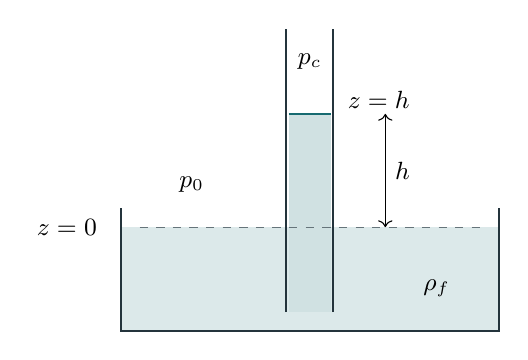
\begin{tikzpicture}[x=1.2cm,y=1.2cm,font=\small]
\fill[accent!15] (-2,-1.1) rectangle (2,0);
\draw[object] (-2,.2)--(-2,-1.1)--(2,-1.1)--(2,.2);
\fill[white] (-.22,0) rectangle (.22,2.1);
\fill[accent!20] (-.22,-.9) rectangle (.22,1.2);
\draw[object] (-.25,-.9)--(-.25,2.1) (.25,-.9)--(.25,2.1);
\draw[accent,thick] (-.22,1.2)--(.22,1.2);
\draw[guide] (-1.8,0)--(1.8,0);
\draw[<->] (.8,0)--(.8,1.2) node[midway,right] {$h$};
\node at (-1.25,.45) {$p_0$};
\node at (0,1.75) {$p_c$};
\node[right] at (1.1,-.65) {$\rho_f$};
\node[left] at (-2.15,0) {$z=0$};
\node[right] at (.3,1.35) {$z=h$};
\end{tikzpicture}
\figcaption{解图 热3.12B　外液面为高度零点；细管上方气压为轴端$p_c$，同一水平液体相通。}
\end{minipage}\end{center}
解图热3.12B的外液面气压为$p_0$，
细管内上升液面的气压为$p_c$。
沿细管液柱由$z=h$下降到$z=0$，压强增加$\rho_fgh$；
在同一相通液体的同一高度应与外侧$p_0$相等：
\[
p_c+\rho_fgh=p_0.
\]
式中用外界压强和轴端压强的差支撑液柱。
代$p_0=n_0kT$及$\rho_a=n_0m$，
\[
h=\frac{p_0}{\rho_fg}\frac{m\omega^2L^2}{6kT}
=\frac{\rho_a\omega^2L^2}{6\rho_fg}.
\]
向上为正，归一化积分$\mathcal F>1$使$p_c<p_0$，
所以h为正，方向与图中的液面上升一致。

\subsubsection*{离心压强梯度与轴端液柱高度}
旋转平衡也满足$\dd p/\dd x=\rho\omega^2x$，
等温时$\rho=mp/(kT)$，积分重得$p(x)=p_c e^{ax^2}$。
在领先阶中可把右边的密度取为未旋转的$\rho_a$，于是
\[
p(x)=p_c+\frac12\rho_a\omega^2x^2+O(\omega^4).
\]
由于温度、体积和气体总量固定，平均压强为$p_0$，
\[
p_0=\frac1L\int_0^Lp(x)\dd x
=p_c+\frac{\rho_a\omega^2L^2}{6}+O(\omega^4).
\]
轴端下降量因此是$\rho_a\omega^2L^2/6$，
远端则比$p_0$高$\rho_a\omega^2L^2/3$。
粗管两端压差为$\rho_a\omega^2L^2/2$。液柱连接的是轴端与外界，实际驱动压差为$p_0-p_c=\rho_a\omega^2L^2/6$，是粗管两端压差的三分之一。
各项单位中$\rho_a\omega^2L^2$为压强，
再除$\rho_fg$得到长度。
积分式按粗管内固定气体体积建立，适用于液面仍在细管中、细管气体体积、气柱重力及毛细效应可忽略的情形。如果液面位移明显改变封闭气体的体积，就把新的体积写入粒子总数方程，再与液柱平衡式联立。


\Needspace{18\baselineskip}

\pdfbookmark[2]{第 13 题 等离子体在引力场中的电场平衡}{q13}

\section*{第 13 题\quad 等离子体在引力场中的电场平衡}

原子序数$Z$、原子量$A$的单质完全电离，正离子质量取$Am_p$、电荷$Ze$，电子质量$m_e$、电荷$-e$。稀薄等离子体在均匀引力场$\bm g$中平衡，局域相互作用忽略。等温时，为使$n_e/n_i=Z$不随位置改变，证明需有均匀电场$\bm E=-(Am_p-m_e)\bm g/[(Z+1)e]$；不等温时若两类粒子每粒子的平均热力相同，也证明此式。太阳表面附近层厚远小于半径，设太阳带均匀表面电荷，求两种条件下的总电荷$Q$。对氢等离子体，取太阳质量$M=2.0\times10^{30}\,\mathrm{kg}$，计算$Q$。

\begin{center}\begin{minipage}{0.96\linewidth}\centering\begin{tikzpicture}[x=1cm,y=1cm,font=\small]
\draw[object,fill=accent!10] (0,1.7) circle (.23);
\node[above left] at (-.2,1.95) {$+Ze,M_i=Am_p$};
\draw[object,fill=warm!10] (4,1.7) circle (.16);
\node[above] at (4,2) {$-e,m_e$};
\draw[force] (0,1.4)--(0,.1) node[left] {$M_ig$};
\draw[motion] (.55,1.7)--(.55,2.8) node[right] {$ZeE$};
\draw[force] (4,1.4)--(4,1) node[left] {$m_eg$};
\draw[motion] (4.55,1.7)--(4.55,.3) node[right] {$eE$};
\draw[axis] (2.1,2)--(2.1,3) node[above] {$\bm E$};
\draw[force] (2.8,2.8)--(2.8,1.9) node[right] {$\bm g$};
\node[below] at (2,-.4) {箭头表示方向，不按大小比例};
\end{tikzpicture}\figcaption{图 热3.13　电场方向向上，使重离子的沉降减弱、电子的沉降增强。}\end{minipage}\end{center}

\Needspace{8\baselineskip}\subsection*{解答}

取$z$竖直向上，重力大小$g$向下，设电场向上且大小$E$。正离子与电子的势能分别为
\[\Phi_i(z)=(Am_pg-ZeE)z,\qquad \Phi_e(z)=(m_eg+eE)z.\]
等温分布$n_i=n_{i0}e^{-\Phi_i/(kT)}$、$n_e=n_{e0}e^{-\Phi_e/(kT)}$。局部准中性使电子数密度为离子的 $Z$ 倍。参考面上 $n_{e0}/n_{i0}=Z$，这个比值沿高度保持时，两种密度的指数斜率相同：
\[Am_pg-ZeE=m_eg+eE.\]
\begin{center}\begin{minipage}{0.96\linewidth}\centering\begin{tikzpicture}[x=1cm,y=1cm,font=\small]
\draw[object,fill=accent!10] (0,1.7) circle (.23);
\node[above left] at (-.2,1.95) {$+Ze,M_i=Am_p$};
\draw[object,fill=warm!10] (4,1.7) circle (.16);
\node[above] at (4,2) {$-e,m_e$};
\draw[force] (0,1.4)--(0,.1) node[left] {$M_ig$};
\draw[motion] (.55,1.7)--(.55,2.8) node[right] {$ZeE$};
\draw[force] (4,1.4)--(4,1) node[left] {$m_eg$};
\draw[motion] (4.55,1.7)--(4.55,.3) node[right] {$eE$};
\draw[axis] (2.1,2)--(2.1,3) node[above] {$\bm E$};
\draw[force] (2.8,2.8)--(2.8,1.9) node[right] {$\bm g$};
\node[below] at (2,-.4) {箭头表示方向，不按大小比例};
\end{tikzpicture}\figcaption{解图 热3.13A　分别列两类粒子的势能梯度或每粒子的力平衡，保持$n_e=Zn_i$。}\end{minipage}\end{center}
解图热3.13A中，向上的电场给正离子向上的电力，却给电子向下的电力。分别沿同一个$z$轴列势能梯度，才有$Am_pg-ZeE$和$m_eg+eE$这两个不同符号。准中性要求两种密度具有相同的衰减指数，因此比较各自的重力与电力合成后所得的势能梯度。

于是
\[E=\frac{Am_p-m_e}{(Z+1)e}g>0,\]
即电场与引力反向，矢量式为
\result{\bm E=-\frac{Am_p-m_e}{(Z+1)e}\bm g.}
电场向上减弱重离子的沉降，同时使电子所受电力向下，令两者具有相同的有效势能梯度。

\textbf{给定的不等温条件。} 设每粒子的平均热力向上且同为$F_{\rm th}$，分别列平衡：
\[F_{\rm th}=Am_pg-ZeE=m_eg+eE.\]
消去它即得相同$E$。消去的是两种粒子共有的平均热力，所以给定的不等温条件下电场也取同一表达式。

\textbf{太阳表面电荷。} 表面外侧的电场向外，说明$Q>0$。太阳半径记为$R_s$，
\[E=\frac{Q}{4\pi\varepsilon_0R_s^2},\qquad g=\frac{GM}{R_s^2}.\]
半径相消，等温和给定不等温条件下均有
\[Q=\frac{4\pi\varepsilon_0G M(Am_p-m_e)}{(Z+1)e}.\]
氢取$A=Z=1$，$\varepsilon_0=8.85419\times10^{-12}\,\mathrm{F/m}$、$G=6.67430\times10^{-11}\,\mathrm{m^3/(kg\cdot s^2)}$、$m_p=1.67262\times10^{-27}\,\mathrm{kg}$、$m_e=9.10938\times10^{-31}\,\mathrm{kg}$、$e=1.60218\times10^{-19}\,\mathrm C$，
\result{Q\simeq77.5\,\mathrm C.}
忽略$m_e$只造成约$5.4\times10^{-4}$的相对修正；有限的表面正电荷提供了此层所需的电场，薄层内仍按局部准中性处理。
\subsubsection*{密度比恒定要求的是指数斜率相同}
令$M_i=Am_p$，仍以向上为z正方向。
解图热3.13A的电场向上，电子电荷为负，故电场力向下；
两类粒子的有效向下力分别为$M_ig-ZeE$与$m_eg+eE$。
图中箭头只标方向，不按不同质量及电荷力的大小比例绘制。
它们对应的密度比为
\[
\frac{n_e(z)}{n_i(z)}
=\frac{n_{e0}}{n_{i0}}
\exp\left\{-\frac{[(m_e-M_i)g+(Z+1)eE]z}{kT}\right\}.
\]
在参考面取$n_{e0}=Zn_{i0}$，
要使所有高度仍有$n_e/n_i=Z$，指数中的 $z$ 系数因此为零。
离子和电子的合成势能沿高度以同一斜率增加，向上的热压力负责支撑这项共同的向下力。
解得E后分别代回，得到共同系数
\[
K=M_ig-ZeE=m_eg+eE
=\frac{M_i+Zm_e}{Z+1}g>0.
\]
于是共同的尺度高度为
\[
H_*=\frac{kT}{K}
=\frac{(Z+1)kT}{(M_i+Zm_e)g},\qquad
\frac{n_i}{n_{i0}}=\frac{n_e}{n_{e0}}=e^{-z/H_*}.
\]

\begin{center}\begin{minipage}{.96\linewidth}\centering
\begin{tikzpicture}[x=1.3cm,y=2.8cm,font=\small]
\draw[axis] (0,0)--(5.6,0) node[right] {$z/H_*$};
\draw[axis] (0,0)--(0,1.22) node[above] {相对参考面密度};
\draw[traj,domain=0:5.2,samples=100] plot (\x,{exp(-\x)});
\draw[warm,thick,dashed,domain=0:5.2,samples=100] plot (\x,{exp(-\x)});
\node[left] at (0,1) {1};
\node[align=center] at (3,.78)
 {$n_i/n_{i0}=n_e/n_{e0}$\\$n_e=Zn_i$};
\end{tikzpicture}
\figcaption{解图 热3.13B　归一化后的两密度曲线重合；一般Z下实际电子数密度是离子的Z倍。}
\end{minipage}\end{center}
用总压强和总质量密度可以直接求 $H_*$。
共同温度下$p=(n_i+n_e)kT=(Z+1)n_i kT$，
质量密度为$\rho=(M_i+Zm_e)n_i$，
所以$p'=-\rho g$给
\[
(Z+1)kT\frac{\dd n_i}{\dd z}
=-(M_i+Zm_e)n_i g,
\]
正好得到同一尺度高度。
求和时离子电荷密度$Zen_i$与电子电荷密度$-en_e$相消，
两组分各自的平衡式仍含方向相反的电场力。

\subsubsection*{不等温时的每粒子平均压强力}
若以连续介质压强描述，向上的每粒子热压力可写成
\[
F_{{\rm th},i}=-\frac1{n_i}\frac{\dd p_i}{\dd z},
\qquad
F_{{\rm th},e}=-\frac1{n_e}\frac{\dd p_e}{\dd z}.
\]
这里的热压力由该组分的压强梯度除以其数密度，表示以单粒子计的平均压力作用。
对共同的非均匀温度T(z)，$p_s=n_s kT$给
\[
F_{{\rm th},s}
=-k\left(T\frac{\dd\ln n_s}{\dd z}
+\frac{\dd T}{\dd z}\right).
\]
若$n_e=Zn_i$且Z不随高度变，二者对数密度梯度相同，
因而这两个每粒子压强力相同，符合题给额外条件。
分别平衡重力和电力后相减，热力消去，仍得同一E。
相减时，共同温度梯度产生的压强项消去，所得电场$E$中不再显含温度梯度。各组分的密度分层仍随温度变化。若两组分温度或热压条件不同，应分别写出各自的压力梯度再求平衡。

\subsubsection*{球面电荷的符号、数值及近似量级}
在太阳表面附近把向上改为径向向外，电场仍与引力相反。
均匀正表面电荷在外侧给$E=Q/(4\pi\varepsilon_0R_s^2)$，
引力为$GM/R_s^2$，比值不含半径。
两种所给热平衡条件都得到同一局部电场，因此代入表面场得到同一 $Q$。
氢的数值代入可写为
\[
Q=\frac{2\pi\varepsilon_0GM(m_p-m_e)}e
\simeq77.5\,\mathrm C.
\]
按给定太阳质量两位有效数字，亦可报约$78\,\mathrm C$；
保留77.5便于比较电子质量修正。
忽略$m_e$所给近似值高于完整值，其相对误差为
\[
\frac{Q_{\rm approx}-Q}{Q}
=\frac{m_e}{m_p-m_e}\simeq5.45\times10^{-4}.
\]
近似只作用于质量差中的电子质量，电子对应的压强与电力仍保留。
若以氢粒子总数约$M/m_p$作数量级比较，
净电荷占一个电子电荷乘总粒子数的比例为
\[
\frac{Q}{eM/m_p}
=\frac{2\pi\varepsilon_0Gm_p(m_p-m_e)}{e^2}.
\]
这一电荷份额极小。局部模型采用准中性的粒子数关系，同时保留少量表面电荷产生的平均场。该场使两种带电组分的分层尺度相同。


\Needspace{18\baselineskip}

\pdfbookmark[2]{第 14 题 自由程分布函数与平均自由程}{q14}

\section*{第 14 题\quad 自由程分布函数与平均自由程}

均匀稀薄气体的自由程模型规定：在已经无碰撞走过任意路程后，再走$\dd\ell$发生碰撞的条件概率为$\dd\ell/a+o(\dd\ell)$，与先前路程无关。求生存概率$F(\ell)$、自由程概率密度$f(\ell)$及平均自由程$\bar\ell $。若已无碰撞走过$\ell_0$，求剩余自由程的分布及平均值。

\begin{center}\begin{minipage}{0.96\linewidth}\centering\begin{tikzpicture}[x=1cm,y=1cm,font=\small,every node/.append style={align=center}]\draw[axis] (0,0)--(6,0) node[right]{$\ell$};\fill[ink] (0,0) circle(2pt);\node[below] at (0,0){上次碰撞};\draw[motion] (0,.4)--(4,.4);\draw[object] (4,-.2)--(4,.6);\node[above] at (4,.6){首次碰撞};\end{tikzpicture}\figcaption{图 热3.14　自由程从上次碰撞的位置计到下次碰撞。}\end{minipage}\end{center}

\Needspace{8\baselineskip}\subsection*{解答}

生存概率$F(\ell)$是走过$\ell$而尚未碰撞的概率。题设的小段条件概率给
\[F(\ell+\dd\ell)=F(\ell)\left(1-\frac{\dd\ell}{a}\right)+o(\dd\ell),\]
\[F'(\ell)=-\frac{F(\ell)}a,\qquad F(0)=1.\]
因此$F(\ell)=e^{-\ell/a}$。自由程落在$[\ell,\ell+\dd\ell]$，要先存活到$\ell$再发生碰撞，故
\[f(\ell)\dd\ell=F(\ell)\frac{\dd\ell}a,\quad
f(\ell)=-F'(\ell)=\frac1a e^{-\ell/a},\qquad\ell\ge0.\]
\begin{center}\begin{minipage}{0.96\linewidth}\centering\begin{tikzpicture}[x=1.3cm,y=2.8cm,font=\small]
\draw[axis] (0,0)--(5.6,0) node[right] {$x=\ell/a$};
\draw[axis] (0,0)--(0,1.22) node[above] {无量纲函数};
\draw[traj,domain=0:5.2,samples=100] plot (\x,{exp(-\x)});
\draw[warm,thick,dashed,domain=0:5.2,samples=100] plot (\x,{exp(-\x)});
\node[left] at (0,1) {1};
\node[align=center] at (3,.8) {$F(ax)=e^{-x}$\\$a f(ax)=e^{-x}$};
\end{tikzpicture}\figcaption{解图 热3.14A　两曲线在归一化纵轴上重合；原密度$f$与$F$单位不同。}\end{minipage}\end{center}
解图热3.14A把无量纲生存概率 $F$ 与乘过尺度的密度 $af$ 画在同一轴上。密度 $f$ 的单位是逆长度。密度的积分与平均为
\[\int_0^\infty f(\ell)\dd\ell=1,\quad
\bar\ell =\frac1a\int_0^\infty\ell e^{-\ell/a}\dd\ell=a.\]
分部积分的端点项$-\ell e^{-\ell/a}|_0^\infty=0$，余项为$\int_0^\infty e^{-\ell/a}\dd\ell=a$。

\textbf{剩余自由程。} 解图热3.14B从已经走过的位置重新计量剩余路程。已经存活到$\ell_0$后，再走$s$的条件生存概率
\[\Pr(\ell>\ell_0+s\mid\ell>\ell_0)=\frac{F(\ell_0+s)}{F(\ell_0)}=e^{-s/a}.\]
\begin{center}\begin{minipage}{0.96\linewidth}\centering\begin{tikzpicture}[x=1cm,y=1cm,font=\small]
\draw[axis] (0,0)--(6.2,0) node[right] {路径坐标};
\fill (0,0) circle (1.4pt) node[below] {0};
\fill (2,0) circle (1.4pt) node[below] {$\ell_0$};
\draw[object] (5,-.15)--(5,.2);
\node[below] at (5,0) {$\ell_0+s$};
\draw[<->] (0,.55)--(2,.55) node[midway,above] {已无碰撞走过$\ell_0$};
\draw[motion] (2,1.25)--(5,1.25) node[midway,above] {剩余$s$};
\node[above] at (2,.1) {C};
\node[above] at (5,.2) {下次碰撞};
\node[below] at (2.8,-.8) {$F^*(\ell_0,s)=F(\ell_0+s)/F(\ell_0)$};
\end{tikzpicture}\figcaption{解图 热3.14B　剩余路程从新的起点计量；条件总路程的平均则还要加$\ell_0$。}\end{minipage}\end{center}
故剩余自由程密度仍为$a^{-1}e^{-s/a}$，平均剩余长度仍为$a=\bar\ell $；总自由程在此条件下的平均为 $\ell_0+a$。其中 $\ell_0$ 是已经通过的距离。
\result{F(\ell)=e^{-\ell/\bar\ell },\quad f(\ell)=\bar\ell ^{-1}e^{-\ell/\bar\ell },\quad
\langle s\mid\ell>\ell_0\rangle=\bar\ell .}
指数律建立在恒定的单位路程碰撞危险率上。密度随位置变动或碰撞截面随速率变动时，用相应的局部碰撞率求生存函数。
\subsubsection*{小段条件概率与首次碰撞}
设随机总自由程为L，$\ell$为已经走过的距离。
题给无后效应性是
\[
\Pr(\ell<L\le\ell+\dd\ell\mid L>\ell)
=\frac{\dd\ell}{a}+o(\dd\ell),
\]
这个概率只以仍无碰撞的样本为分母。
首次碰撞落在这一段的分子先无碰撞走到 $\ell$，所以
$\Pr(\ell<L\le\ell+\dd\ell)=F(\ell)\dd\ell/a+o(\dd\ell)$。
累计生存函数$F(\ell)=\Pr(L>\ell)$随$\ell$下降，
微分为负；密度$f=-F'$为正，两者单位分别是1和逆长度。

将微分方程分离变量，并使用起点条件，完整积分为
\[
\int_1^{F(\ell)}\frac{\dd F}{F}
=-\frac1a\int_0^\ell\dd x,\qquad
\ln F(\ell)=-\frac{\ell}{a}.
\]
$a>0$时$F(0)=1$、$F(\infty)=0$，
因此$f=a^{-1}e^{-\ell/a}$自动给
\[
\int_0^\infty f(\ell)\dd\ell
=F(0)-F(\infty)=1.
\]
用每个长度乘该处的概率密度积分，得
\[
\begin{aligned}
\langle L\rangle
&=\frac1a\int_0^\infty\ell e^{-\ell/a}\dd\ell\\
&=[-\ell e^{-\ell/a}]_0^\infty
+\int_0^\infty e^{-\ell/a}\dd\ell=a.
\end{aligned}
\]
也可由非负随机变量的尾积分公式
$\langle L\rangle=\int_0^\infty F(\ell)\dd\ell=a$ 得到同一均值。

\subsubsection*{从新起点计算条件密度与均值}
解图热3.14B中已存活到C点$\ell_0$，
新的路程变量为$s=L-\ell_0$。
在已经存活的样本中，条件生存函数与密度分别为
\[
F^*(\ell_0,s)=\frac{F(\ell_0+s)}{F(\ell_0)}
=e^{-s/a},
\]
\[
f^*(\ell_0,s)=\frac{f(\ell_0+s)}{F(\ell_0)}
=\frac1a e^{-s/a},\qquad s\ge0.
\]
后一式既可从条件概率求，也可对前式取负导数。
分母 $F(\ell_0)$ 把概率换成以存活样本为总体的比例。
平均剩余自由程是
\[
\langle s\mid L>\ell_0\rangle
=\int_0^\infty s f^*(\ell_0,s)\dd s=a,
\]
而条件总长度的密度为
\[
f_{L\mid L>\ell_0}(L)
=\frac1a e^{-(L-\ell_0)/a},\qquad L\ge\ell_0,
\]
故$\langle L\mid L>\ell_0\rangle=\ell_0+a$。
平均剩余长度虽不变，总长度仍包括已经走过的$\ell_0$。

\subsubsection*{指数律的尺度、涨落与模型范围}
解图热3.14A以$x=\ell/a$为横轴，
画的是无量纲密度$a f(ax)$与生存概率$F(ax)$；
这两条函数在本模型中恰好都等于$e^{-x}$。
乘尺度 $a$ 将逆长度量纲的 $f$ 换成无量纲的纵轴。
指数自由程不是固定步长：
\[
\Pr(L>a)=e^{-1},\qquad
L_{\rm median}=a\ln2,\qquad
\langle L^2\rangle=2a^2,\qquad
\operatorname{Var}(L)=a^2.
\]
超过平均值的概率约为$36.8\%$，标准差也为a，
说明每次自由程可以显著不同。

若单位路程危险率为位置函数$\kappa(x)$，
则$F'=-\kappa F$给
\[
F(\ell)=\exp\left[-\int_0^\ell\kappa(x)\dd x\right],
\quad
\frac{F(\ell_0+s)}{F(\ell_0)}
=\exp\left[-\int_{\ell_0}^{\ell_0+s}\kappa(x)\dd x\right].
\]
剩余分布一般会依赖起点$\ell_0$。
即使不同子样本各有恒定危险率，混合后也未必无记忆。
例如两个尺度$a_1,a_2$按比例q和$1-q$混合，
生存函数为$q e^{-\ell/a_1}+(1-q)e^{-\ell/a_2}$；
已存活较长距离的样本中，较大尺度的那一组所占比例增加。条件均值用更新后的各组比例计算。
本题的单位路程危险率恒定，因而同一指数模型可用于每个新的观测起点。


\Needspace{18\baselineskip}

\pdfbookmark[2]{第 15 题 分子随机游走位移与扩散时间}{q15}

\section*{第 15 题\quad 分子随机游走位移与扩散时间}

理想气体的平均速率$\bar v$、平均自由程$\bar\ell $已知。以某分子初始位置为原点，按方向独立、自由程为指数分布的随机游走模型，估算方均位移等于$R^2$的特征时间。设$R\gg\bar\ell $，容器足够大，讨论期间未撞壁。给定$\bar v=5.0\times10^2\,\mathrm{m/s}$、$\bar\ell =3.0\times10^{-7}\,\mathrm m$、$R=2\,\mathrm m$，求数值；说明它与单次轨迹的首次到达时间有何区别。

\begin{center}\begin{minipage}{0.96\linewidth}\centering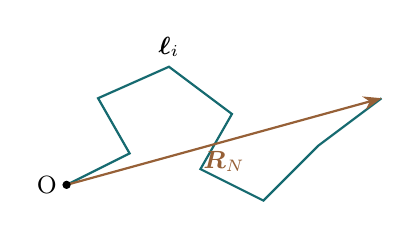
\begin{tikzpicture}[x=1cm,y=1cm,font=\small,every node/.append style={align=center}]\draw[traj] (0,0)--(.8,.4)--(.4,1.1)--(1.3,1.5)--(2.1,.9)--(1.7,.2)--(2.5,-.2)--(3.2,.5)--(4,1.1);\draw[force] (0,0)--(4,1.1) node[midway,below]{$\bm R_N$};\fill (0,0) circle(1.5pt);\node[left] at (0,0){O};\node[above] at (1.3,1.5){$\bm\ell_i$};\end{tikzpicture}\figcaption{图 热3.15　实际行程为折线路径，位移是首尾之间的矢量。}\end{minipage}\end{center}

\Needspace{8\baselineskip}\subsection*{解答}

设第$i$段自由程矢量为$\bm\ell_i$，经过$N$段后的位移$\bm R_N=\sum_{i=1}^N\bm\ell_i$。方向独立且各向同性，所以$\langle\bm\ell_i\rangle=0$，$i\ne j$时交叉平均$\langle\bm\ell_i\cdot\bm\ell_j\rangle=0$。
\[\langle R_N^2\rangle=\sum_i\langle\ell_i^2\rangle
+2\sum_{i<j}\langle\bm\ell_i\cdot\bm\ell_j\rangle=N\langle\ell^2\rangle.\]
\begin{center}\begin{minipage}{0.96\linewidth}\centering\begin{tikzpicture}[x=1cm,y=1cm,font=\small,every node/.append style={align=center}]\draw[traj] (0,0)--(.8,.4)--(.4,1.1)--(1.3,1.5)--(2.1,.9)--(1.7,.2)--(2.5,-.2)--(3.2,.5)--(4,1.1);\draw[force] (0,0)--(4,1.1) node[midway,below]{$\bm R_N$};\fill (0,0) circle(1.5pt);\node[left] at (0,0){O};\node[above] at (1.3,1.5){$\bm\ell_i$};\node[below] at (2,-.8){交叉项仅在统计平均后相消};\end{tikzpicture}\figcaption{解图 热3.15A　独立方向的各步对位移二阶矩分别作贡献。}\end{minipage}\end{center}
解图热3.15A的折线是许多自由程矢量的首尾相接，起终点的连线才是$\bm R_N$。平方展开时，每个折线段贡献$\langle\ell^2\rangle$，不同段之间的交叉项在方向平均后消失。解图热3.15B的直线于是表示统计二阶矩随时间增长。横轴给统计记录的经过时间。

对单次轨迹，交叉项由折线段之间的夹角决定。对许多独立方向的轨迹取平均，任意一段在另一段方向上的平均投影为零。由指数自由程分布，
\[\langle\ell^2\rangle=\frac1{\bar\ell }\int_0^\infty\ell^2e^{-\ell/\bar\ell }\dd\ell.\]
令$y=\ell/\bar\ell $，两次分部积分给
\[\int_0^\infty y^2e^{-y}\dd y=2\int_0^\infty ye^{-y}\dd y=2,
\qquad\langle\ell^2\rangle=2\bar\ell ^2.\]
以平均碰撞频率$\bar Z=\bar v/\bar\ell $作长时间估算，$N\simeq\bar Zt$，所以
\[\langle R^2(t)\rangle\simeq2\bar v\bar\ell  t=6Dt,\qquad D\simeq\frac{\bar v\bar\ell }{3}.\]
\begin{center}\begin{minipage}{0.96\linewidth}\centering\begin{tikzpicture}[x=4cm,y=3cm,font=\small]
\draw[axis] (0,0)--(1.6,0) node[right] {$t/t_R$};
\draw[axis] (0,0)--(0,1.6) node[above] {$\langle R^2(t)\rangle/R^2$};
\draw[traj] (0,0)--(1.45,1.45);
\draw[guide] (1,0)--(1,1)--(0,1);
\node[below] at (1,0) {1};
\node[left] at (0,1) {1};
\node[align=center] at (.55,1.35) {长时间扩散近似\\$t_R=R^2/(2\bar v\bar\ell)$};
\end{tikzpicture}\figcaption{解图 热3.15B　线性方均位移给扩散特征时间，不给单条轨迹的确定到达时刻。}\end{minipage}\end{center}
令方均位移等于$R^2$，得到
\result{t\simeq\frac{R^2}{2\bar v\bar\ell }.}
数值为
\[t=\frac{2^2}{2\times5.0\times10^2\times3.0\times10^{-7}}
=1.333\times10^4\,\mathrm s\simeq3.7\,\mathrm h.\]
无碰撞直线飞行所需时间为 $R/\bar v=0.004\,\mathrm s$。在随机游走中，约3.7h对应许多轨迹的方均位移达到 $R^2$。指定目标面后，每条轨迹分别给出其首次到达时间。若改用固定步长为 $\bar\ell$ 的模型，步长二阶矩减为指数模型的一半。
\subsubsection*{先对矢量和作统计平均，再引入典型距离}
解图热3.15A的每个折线段有三个投影，
对一条具体轨迹可写
\[
R_N^2=\left(\sum_i\ell_{ix}\right)^2+
\left(\sum_i\ell_{iy}\right)^2+
\left(\sum_i\ell_{iz}\right)^2.
\]
各向同性给每段平均投影为零，独立方向使不同段交叉平均为零。
对三个方向分别平均再相加，得
\[
\begin{aligned}
\langle R_N^2\rangle
&=\sum_i\bigl(\langle\ell_{ix}^2\rangle+
\langle\ell_{iy}^2\rangle+\langle\ell_{iz}^2\rangle\bigr)\\
&=N\langle\ell^2\rangle,\qquad
\langle X_N^2\rangle=\frac13N\langle\ell^2\rangle.
\end{aligned}
\]
每条轨迹有自己的投影乘积和位移平方。对同一模型的大量轨迹取平均，交叉项的正负贡献才相互抵消。

用自由程分布直接求平方的平均。
记$a=\bar\ell$，其不定积分可显式写成
\[
\int\frac{\ell^2}{a}e^{-\ell/a}\dd\ell
=-(\ell^2+2a\ell+2a^2)e^{-\ell/a}+C.
\]
无穷端指数压过多项式，零端为$-2a^2$，
故$\langle\ell^2\rangle=2a^2$。
指数自由程的均方等于均值平方 $a^2$ 加方差 $a^2$。固定步长时方差为零，因此两模型的二阶矩相差一倍。

\subsubsection*{由同一记录的总量联系步数与时间}
在足够长的统计记录中，记总实际行程为$\mathcal L$、
完成的自由程段数为N、总时间为t。
用同一记录定义
\[
\bar\ell\simeq\frac{\mathcal L}{N},\qquad
\bar v\simeq\frac{\mathcal L}{t},\qquad
\bar Z\simeq\frac Nt.
\]
三式相除给$\bar Z=\bar v/\bar\ell$，
因为三个量都由同一次长期记录的总量定义。
若用每段飞行时间$\tau_i$表示，
应先有$\bar\tau=\langle\tau_i\rangle$、$\bar Z=1/\bar\tau$，
并保持时间平均速率与逐碰撞平均长度的口径一致。
在独立方向、有限步长二阶矩的长时间更新模型中，
\[
\langle R^2(t)\rangle\simeq
\frac{\langle\ell^2\rangle}{\bar\tau}t,\qquad
D=\frac{\langle\ell^2\rangle}{6\bar\tau}.
\]
代指数步长的二阶矩和同一记录的计数关系，才得到前面的$D=\bar v\bar\ell/3$。
最后一段尚未完成的飞行和起始瞬态在长时间主要项中可忽略；
短于碰撞时间时应改用弹道增长$\langle R^2\rangle\simeq\langle v^2\rangle t^2$。
解图热3.15B只表示长时间扩散近似。

本题可依次算出
\[
\bar Z=\frac{500}{3.0\times10^{-7}}
=1.67\times10^9\,\mathrm{s^{-1}},\qquad
\bar\tau=6.0\times10^{-10}\,\mathrm s,
\]
\[
N_R=\frac{R^2}{2\bar\ell^2}=2.22\times10^{13},\qquad
D=5.0\times10^{-5}\,\mathrm{m^2/s}.
\]
于是$N_R/\bar Z=R^2/(6D)=1.333\times10^4\,\mathrm s$，
约为3.7 h；这一时间内累计行程约$N_R\bar\ell=6.7\times10^6\,\mathrm m$，
但净位移尺度只有2 m。
条件$R/\bar\ell\simeq6.7\times10^6\gg1$，
对应很多次碰撞的长时间尺度。

\subsubsection*{方均位移时间与首次碰到球面的时间}
\begin{center}\begin{minipage}{.96\linewidth}\centering
\begin{tikzpicture}[x=1.1cm,y=1.1cm,font=\small]
\draw[object] (0,0) circle (2);
\draw[traj] (0,0)--(-.7,.3)--(-.5,1.1)--(.5,1.3)
 --(1,.4)--(1.6,.6)--(2,0);
\fill (0,0) circle (1.3pt) node[below left] {O};
\fill (2,0) circle (1.3pt) node[right] {首次接触};
\draw[force,<->] (0,0)--(0,-2) node[midway,right] {$R$};
\node[above] at (0,2.2) {球形吸收面的截面};
\end{tikzpicture}
\figcaption{解图 热3.15C　若另规定在半径R的球面停止，首次到达时间仍因轨迹而异。}
\end{minipage}\end{center}
题目所算$t_R$由$\langle R^2(t_R)\rangle=R^2$定义，
它描述所有粒子的位移涨落。
若进一步采用三维连续扩散模型，并指定解图热3.15C的球面为吸收面，
可以另求平均首次到达时间$\tau(r)$。
它满足
\[
D\left(\tau''+\frac2r\tau'\right)=-1,\qquad
\tau(R)=0,\quad \tau(0)\ \text{有限}.
\]
积分$r^2\tau'=-r^3/(3D)$，再用球面条件得
\[
\tau(r)=\frac{R^2-r^2}{6D},\qquad \tau(0)=\frac{R^2}{6D}.
\]
所以在这一特定球形、无漂移扩散模型中，平均首次到达时间的数值恰与方均位移时间相同；
前者用固定时刻的位移平方取平均，后者对各轨迹的随机首次到达时刻取平均。改变目标面形状、起始位置或漂移后，首次到达时间由相应的扩散方程求出。


\Needspace{18\baselineskip}

\pdfbookmark[2]{第 16 题 混合气体中两类分子的平均自由程}{q16}

\section*{第 16 题\quad 混合气体中两类分子的平均自由程}

温度$T$下的平衡混合理想气体包含A、B两种硬球分子，质量$m_A,m_B$，有效直径$d_A,d_B$，数密度$n_A,n_B$。求两类分子各自的平均自由程$\bar\ell _A,\bar\ell _B$；碰撞频率须包括同类、异类两部分，并考虑相对速率。

\begin{center}\begin{minipage}{0.96\linewidth}\centering\begin{tikzpicture}[x=1.2cm,y=1.2cm,font=\small]
\draw[guide] (0,0) circle (1.5);
\draw[object,fill=warm!8] (0,0) circle (.9);
\draw[object,fill=accent!8] (0,1.5) circle (.6);
\fill (0,0) circle (1.2pt);
\fill (0,1.5) circle (1.2pt);
\node[above] at (0,2.25) {A，半径$d_A/2$};
\node[below] at (0,-1.05) {B，半径$d_B/2$};
\draw[guide] (-2.1,1.5)--(-.65,1.5);
\draw[motion] (-2,1.5)--(-.8,1.5) node[midway,above] {$\bm u_{AB}$};
\draw[guide] (0,0)--(1.8,0) (0,1.5)--(1.8,1.5);
\draw[<->] (1.8,0)--(1.8,1.5) node[midway,right] {$b_{\max}=(d_A+d_B)/2$};
\end{tikzpicture}\figcaption{图 热3.16　碰撞取决于两球中心距离与两半径之和。}\end{minipage}\end{center}

\Needspace{8\baselineskip}\subsection*{解答}

异类硬球的碰撞截面由两球中心距离小于半径之和决定，
\[\sigma_{AB}=\pi\left(\frac{d_A+d_B}{2}\right)^2,
\quad\sigma_{AA}=\pi d_A^2,\quad\sigma_{BB}=\pi d_B^2.\]
\begin{center}\begin{minipage}{0.96\linewidth}\centering\begin{tikzpicture}[x=1.2cm,y=1.2cm,font=\small]
\draw[guide] (0,0) circle (1.5);
\draw[object,fill=warm!8] (0,0) circle (.9);
\draw[object,fill=accent!8] (0,1.5) circle (.6);
\fill (0,0) circle (1.2pt);
\fill (0,1.5) circle (1.2pt);
\node[above] at (0,2.25) {A，半径$d_A/2$};
\node[below] at (0,-1.05) {B，半径$d_B/2$};
\draw[guide] (-2.1,1.5)--(-.65,1.5);
\draw[motion] (-2,1.5)--(-.8,1.5) node[midway,above] {$\bm u_{AB}$};
\draw[guide] (0,0)--(1.8,0) (0,1.5)--(1.8,1.5);
\draw[<->] (1.8,0)--(1.8,1.5) node[midway,right] {$b_{\max}=(d_A+d_B)/2$};
\end{tikzpicture}\figcaption{解图 热3.16A　固定B中心时，A中心经过等效圆盘就发生碰撞；同类与异类频率分别计算。}\end{minipage}\end{center}
解图热3.16A固定B分子的中心后，A中心只要进入半径$(d_A+d_B)/2$的圆盘就发生接触，所以截面要取这一个半径的平方。A遇到A、B两类靶的事件互不替代，频率应相加；求A自身的平均自由程时，分子取$\bar v_A$，各碰撞项则分别使用相应的相对平均速率。

单分子平均速率和异类相对平均速率为
\[\bar v_A=\sqrt{\frac{8kT}{\pi m_A}},\quad
\bar v_B=\sqrt{\frac{8kT}{\pi m_B}},\quad
\bar u_{AB}=\sqrt{\frac{8kT}{\pi}\left(\frac1{m_A}+\frac1{m_B}\right)}.\]
同类相对平均速率为$\sqrt2\bar v_A$或$\sqrt2\bar v_B$。追踪一个A分子时，两种靶的频率相加：
\[\bar Z_{AA}=n_A\pi d_A^2\sqrt2\bar v_A,\qquad
\bar Z_{AB}=n_B\frac\pi4(d_A+d_B)^2\bar u_{AB},\]
\[\bar Z_A=\bar Z_{AA}+\bar Z_{AB},\qquad
\bar\ell _A=\frac{\bar v_A}{\bar Z_A}.\]
利用$\bar u_{AB}/\bar v_A=\sqrt{1+m_A/m_B}$，得到
\result{\bar\ell _A=\left[\sqrt2\pi d_A^2n_A+
\frac\pi4(d_A+d_B)^2n_B\sqrt{1+\frac{m_A}{m_B}}\right]^{-1}.}
同理
\result{\bar\ell _B=\left[\sqrt2\pi d_B^2n_B+
\frac\pi4(d_A+d_B)^2n_A\sqrt{1+\frac{m_B}{m_A}}\right]^{-1}.}
此平均指总行程除以总碰撞次数，即平均速率除以每粒子平均碰撞频率。全体A—A事件由两个参与者同时记录，所以总参与次数除以2得到事件数。跟踪单个A时，它每参加一次碰撞就结束一个自由程。若两类质量、直径相同，两式都回到$[\sqrt2\pi d^2(n_A+n_B)]^{-1}$，在固定密度的此硬球模型中温度因子相消。
\subsubsection*{接触距离与碰撞截面的几何}
解图热3.16A中两球恰接触时，中心间距为
$b_{\max}=d_A/2+d_B/2$。
在相对运动描述中固定B中心，
A中心的入射轨迹若有横向碰撞参数$b<b_{\max}$便会碰到B；
达到 $b=b_{\max}$ 时两球刚好相切。
接触距离是长度，碰撞截面则是垂直相对速度的平面内全部允许碰撞参数所占面积：
\[
\sigma_{AB}=\pi b_{\max}^2=\frac\pi4(d_A+d_B)^2.
\]

\begin{center}\begin{minipage}{.96\linewidth}\centering
\begin{tikzpicture}[x=1.2cm,y=1.2cm,font=\small]
\fill[accent!15] (0,0) circle (1.5);
\draw[object] (0,0) circle (1.5);
\fill (0,0) circle (1.3pt) node[below left] {O};
\draw[<->] (0,0)--(1.5,0) node[midway,above] {$b_{\max}$};
\node at (-.6,.7) {$\sigma_{AB}$};
\node[above,align=center] at (0,1.8)
 {垂直$\bm u_{AB}$的碰撞参数平面};
\node[below] at (0,-1.9) {$b<b_{\max}$的面积为$\pi b_{\max}^2$};
\end{tikzpicture}
\figcaption{解图 热3.16B　碰撞圆盘的半径已经合计两球的半径。}
\end{minipage}\end{center}
同类时$d_A=d_B$，中心接触距离为$d_A$，
所以截面为 $\sigma_{AA}=\pi d_A^2$，对应两个相同半径之和。
解图热3.16B先完成半径相加，再平方求面积；
把直径相加直接当半径，会使截面大四倍。

\subsubsection*{分别计算各类靶的碰撞频率}
以A为被追踪分子，A靶与B靶的密度分别为$n_A,n_B$，
相对速率分别为$\sqrt2\bar v_A$与$\bar u_{AB}$。
异类相对速率通过约化质量
$\mu_{AB}=m_Am_B/(m_A+m_B)$给出。
因此
\[
\bar Z_A=n_A\sigma_{AA}\sqrt2\bar v_A
+n_B\sigma_{AB}\sqrt{\frac{8kT}{\pi\mu_{AB}}}.
\]
求A的实际平均行程，以被追踪的A分子的平均速率 $\bar v_A$ 作分子。
约去共同速度尺度时，两个异类速率比分别为
\[
\frac{\bar u_{AB}}{\bar v_A}
=\sqrt{\frac{m_A}{\mu_{AB}}}
=\sqrt{\frac{m_A+m_B}{m_B}},\qquad
\frac{\bar u_{AB}}{\bar v_B}
=\sqrt{\frac{m_B}{\mu_{AB}}}
=\sqrt{\frac{m_A+m_B}{m_A}}.
\]
故$\bar\ell_A$与$\bar\ell_B$互换A、B标号，但一般并不相等。
分母中每项都是数密度乘面积再乘无量纲速率比，
单位为逆长度，所以倒数是长度。

\subsubsection*{平均自由程和碰撞计数的统一口径}
在一段长的平稳记录中，设A分子的总实际行程为$\mathcal L_A$，
参与碰撞总次数为$C_A$，记录时间为t，则
\[
\bar\ell_A=\frac{\mathcal L_A}{C_A},\qquad
\bar v_A=\frac{\mathcal L_A}{t},\qquad
\bar Z_A=\frac{C_A}{t}.
\]
所以$\bar\ell_A=\bar v_A/\bar Z_A$是这些平均定义之间的恒等关系，
式中的两个平均都来自同一份记录。
若固定A的瞬时速度$\bm v$，
碰撞频率应先对靶的速度积分：
\[
Z_A(\bm v)=\sum_{j=A,B}n_j\sigma_{Aj}
\int|\bm v-\bm w|f_j(\bm w)\dd^3w.
\]
再按A的平衡速度密度对$\bm v$平均，
才得到$n_j\sigma_{Aj}\langle u_{Aj}\rangle$的各项。
实际参加碰撞的速度样本还按事件发生率加权，
逐次碰撞的速度平均按事件率加权，随机时刻的平均则按时间取样。若还要求全体分子的自由程分布，应把不同速率对应的危险率和各自权重一起计入。

若统计每单位体积每单位时间的所有碰撞事件，
同类事件须消除两次参与计数，而异类每对只计一次：
\[
\mathcal C_{AA}=\frac12n_A\bar Z_{AA},\qquad
\mathcal C_{BB}=\frac12n_B\bar Z_{BB},\qquad
\mathcal C_{AB}=n_A\bar Z_{AB}=n_B\bar Z_{BA}.
\]
但追踪某个A分子时，它每参加一次AA碰撞都确实结束一个自由程，
它的 $\bar Z_{AA}$ 直接按参与次数计。

\subsubsection*{纯组分、相同标号和重靶极限}
当$n_B\to0$时，A式回到
$\bar\ell_A=1/(\sqrt2\pi d_A^2n_A)$。
若两种只是相同质量、相同直径分子的不同标号，
异类相对速率也为$\sqrt2\bar v$，
两式都只含总密度$n_A+n_B$，两种标号合并后得到同一结果。
若$m_B/m_A\to\infty$且$n_A,n_B$保持正，
A对B的速率比趋1，B可在A的碰撞估计中视为静止重靶；
反过来，B仍受运动A的碰撞，其自身平均行程随$\bar v_B$趋零而可变短，
只要 $n_A>0$，运动A造成的每秒碰撞次数仍有有限极限。若先令 $n_A=0$，纯B气体的自由程由其数密度和截面决定，与质量无关。

硬球截面与速率无关，固定$n_A,n_B$时所有平均热速都含相同$\sqrt T$，
故自由程中的温度因子约去。
若实验保持各组分分压，$n_j=p_j/(kT)$随T改变，
自由程便与T成正比。


\Needspace{18\baselineskip}

\pdfbookmark[2]{第 17 题 阴极射线管真空度与电子无碰撞概率}{q17}

\section*{第 17 题\quad 阴极射线管真空度与电子无碰撞概率}

阴极射线管长$L=20\,\mathrm{cm}$，残余空气温度27℃，分子有效直径$d=3.0\times10^{-10}\,\mathrm m$。电子尺寸忽略，电子速度远大于分子热速。为使至少90\%的电子不经碰撞到达荧光屏，求残余空气压强上限。用几何遮挡模型说明无碰撞概率的指数形式。

\begin{center}\begin{minipage}{0.96\linewidth}\centering\begin{tikzpicture}[x=1cm,y=1cm,font=\small,every node/.append style={align=center}]\draw[object] (0,0) rectangle(6,2);\draw[object,line width=2pt] (5.8,0)--(5.8,2);\node[left] at (0,1){阴极};\node[right] at (6,1){屏};\draw[motion] (.2,1)--(5.6,1);\foreach \x/\y in {1/.3,2/1.6,3/.7,4/1.4,5/.2}{\draw[object] (\x,\y) circle(.11);}\node[below] at (3,-.4){$L=20$ cm};\end{tikzpicture}\figcaption{图 热3.17　残余空气分子可能截断电子的直达轨迹。}\end{minipage}\end{center}

\Needspace{8\baselineskip}\subsection*{解答}

电子相对空气分子极快，可把靶分子近似看作静止，且电子的几何半径忽略。碰撞中心距离由靶分子半径决定，因此截面为 $\sigma=\pi(d/2)^2$。靶分子近似静止时，相对速率就是电子的速率。
\begin{center}\begin{minipage}{0.96\linewidth}\centering\begin{tikzpicture}[x=1cm,y=1cm,font=\small]
\draw[object] (0,0) rectangle (6,2);
\draw[object,line width=2pt] (5.8,0)--(5.8,2);
\node[left] at (0,1) {阴极};
\node[right] at (6,1) {屏};
\draw[motion] (.2,1)--(5.8,1);
\foreach \x/\y in {1.2/.3,2.1/1.7,3.5/.4,4.4/1.6,5.2/.2}
 {\draw[object] (\x,\y) circle (.22);}
\draw[guide] (.2,.78)--(5.8,.78) (.2,1.22)--(5.8,1.22);
\draw[<->] (.2,-.4)--(5.8,-.4) node[midway,below] {$L=20\,\mathrm{cm}$};
\node[above] at (3,2.3) {候选碰撞管半径$r=d/2$};
\end{tikzpicture}\figcaption{解图 热3.17A　电子视为点粒子，几何截面与空气分子的半径对应。}\end{minipage}\end{center}
解图热3.17A中从阴极到屏的长度为$L$，沿轨迹扫出的碰撞管半径只有空气分子半径$d/2$。将这根管分成许多薄片，每片的存活概率相乘，连续极限才给$P_0=e^{-n\sigma L}$；将这个生存概率与要求的最低透过率比较，可求允许的最高压强。

扫过长$L$、面积$\sigma$的碰撞管，泊松模型给生存概率
\[P_0(L)=e^{-n\sigma L}=e^{-L/\bar\ell _e},\qquad\bar\ell _e=(n\sigma)^{-1}.\]
\textbf{几何遮挡的指数极限。} 以间距$a$、横向位置相互独立随机的稀疏靶层说明，每层未遮住的面积比$1-\sigma/a^2$，穿过$L/a$层的概率
\[\left(1-\frac\sigma{a^2}\right)^{L/a}\simeq
\exp\left(-\frac{\sigma L}{a^3}\right)=e^{-n\sigma L},\qquad n=a^{-3}.\]
这里的层距用于把上一式写成数密度，横向位置仍取彼此独立的随机分布。对生存概率求导得首次碰撞密度$n\sigma e^{-n\sigma x}$，积分期望同为$\bar\ell _e=1/(n\sigma)$。

要求$P_0\ge0.90$，则$\bar\ell _e\ge-L/\ln0.90=1.89824\,\mathrm m$。因$p=nkT$，
\[p\le\frac{-kT\ln0.90}{\sigma L}
=\frac{-1.380649\times10^{-23}\times300.15\ln0.90}
{\pi(1.5\times10^{-10})^2\times0.20}.\]
\result{p\le3.09\times10^{-2}\,\mathrm{Pa}.}
压强决定靶分子的数密度。用题设直径算出的几何截面固定时，压强越低，解图热3.17A的碰撞管内平均包含的分子越少，直达率越高。上式取的是直达率恰为 $90\%$ 的压强。
\subsubsection*{从候选碰撞体积推导指数生存概率}
解图热3.17A中电子按点粒子处理，
若空气分子中心距候选电子直线小于$r=d/2$就会碰撞。
因此围绕这条线作半径r的碰撞管，截面为$\sigma=\pi r^2$。
无碰撞直达的事件是整根候选碰撞管内的靶中心数为零。
电子速度远大于分子热速，使通过期间近似冻结靶的位置；
若截面按题给硬球几何固定，速度在“每秒碰撞次数除以每秒行程”中相消。

\begin{center}\begin{minipage}{.96\linewidth}\centering
\begin{tikzpicture}[x=1cm,y=1cm,font=\small]
\fill[accent!12] (3.4,-.8) rectangle (4,.8);
\draw[object] (0,0) ellipse (.25 and .8);
\draw[object] (4,0) ellipse (.25 and .8);
\draw[guide] (3.4,0) ellipse (.25 and .8);
\draw[object] (0,-.8)--(4,-.8) (0,.8)--(4,.8);
\draw[motion] (-.8,0)--(4.8,0);
\draw[<->] (3.4,-1.15)--(4,-1.15) node[midway,below] {$\Delta x$};
\node[above] at (3.7,1.1) {薄层体积$\sigma\Delta x$};
\node[above] at (1.2,.95) {$\sigma=\pi(d/2)^2$};
\end{tikzpicture}
\figcaption{解图 热3.17B　独立稀薄层中的候选碰撞数与$n\sigma\Delta x$成正比。}
\end{minipage}\end{center}
把长度L分成M个很薄的独立稀薄层，$\Delta x=L/M$。
每层候选体积$\sigma\Delta x$中的靶数平均为$n\sigma\Delta x$，
在泊松位置模型下，至少一个靶的概率到一阶即为该值。
因此
\[
P_0(L)=\lim_{M\to\infty}
\left(1-\frac{n\sigma L}{M}\right)^M
=e^{-n\sigma L}.
\]
这也可由$P_0'(x)=-n\sigma P_0(x)$、$P_0(0)=1$得到。
层间独立是这里的统计条件。
若假设完美对齐的静止立方晶格，电子又严格垂直同向穿层，
不同层的阴影会完全重合，避开第一层也就避开其余同样对齐的靶。这时总存活概率由一层的未遮挡面积比给出。
以层距$a_c$描述的稀薄层模型，应另让横向位置独立随机，
此时每层存活约$1-\sigma/a_c^2$，
穿过$L/a_c$层才给
$\exp[-\sigma L/a_c^3]$，并以$n=a_c^{-3}$联系数密度。
各层独立的横向位置使未遮住的概率相乘。

\subsubsection*{由首次碰撞密度求平均自由程}
记$\kappa=n\sigma$，生存函数为$P_0(x)=e^{-\kappa x}$，
首次碰撞位于$[x,x+\dd x]$的概率为
\[
f_e(x)\dd x=-P_0'(x)\dd x
=\kappa e^{-\kappa x}\dd x,\qquad x\ge0.
\]
其归一化与均值分别为
\[
\int_0^\infty\kappa e^{-\kappa x}\dd x=1,
\]
\[
\begin{aligned}
\bar\ell_e
&=\int_0^\infty x\kappa e^{-\kappa x}\dd x\\
&=[-xe^{-\kappa x}]_0^\infty+
\int_0^\infty e^{-\kappa x}\dd x=\frac1\kappa.
\end{aligned}
\]
平均自由程是首次碰撞距离的期望，积分将所有可能的碰撞距离加权。
事实上到$x=\bar\ell_e$的累计碰撞概率仅为$1-e^{-1}$，
而剩下$e^{-1}$的样本还没有碰撞。
若电子速率为$v_e$，单位时间扫过体积$\sigma v_e$，
故$\bar Z_e=n\sigma v_e$、$\bar\ell_e=v_e/\bar Z_e=1/(n\sigma)$，
与密度积分路线一致。

\subsubsection*{由允许碰撞厚度求压强上限}
定义无量纲碰撞厚度$\Lambda=n\sigma L$。
要求至少90\%无碰撞就是
\[
e^{-\Lambda}\ge0.90,\qquad
\Lambda\le-\ln0.90=0.1053605.
\]
对透过率取负对数可求碰撞厚度。取对数后乘以负数会改变不等号方向，
所以允许密度和压强均是上限，而平均自由程是下限：
\[
n\le\frac{-\ln0.90}{\sigma L},\qquad
\bar\ell_e\ge\frac{L}{-\ln0.90}=9.4912L.
\]
代$L=0.20\,\mathrm m$、$r=1.5\times10^{-10}\,\mathrm m$，
\[
\sigma=7.0686\times10^{-20}\,\mathrm{m^2},\qquad
n_{\max}\simeq7.45\times10^{18}\,\mathrm{m^{-3}},
\]
\[
T=27+273.15=300.15\,\mathrm K,\qquad
p_{\max}=n_{\max}kT\simeq0.0309\,\mathrm{Pa}.
\]
若恰取上限，$\bar\ell_e\simeq1.90\,\mathrm m$；
取更低压强只会提高无碰撞透过率。
若误令$\bar\ell_e=L$，实际透过率只有$e^{-1}\simeq36.8\%$，
远未满足90\%的要求。

本题电子与静止大靶的截面为$\pi d^2/4$。
空气分子彼此碰撞的截面为$\pi d^2$，
还因双方热运动出现$\sqrt2$相对速率因子。
因此同一数密度下
\[
\frac{\bar\ell_e}{\bar\ell_{\rm air}}
=\frac{4/(\pi d^2n)}{1/(\sqrt2\pi d^2n)}
=4\sqrt2.
\]
高速点电子与气体分子自身对应不同的碰撞几何及相对速率。
如果数密度沿管长变化，独立模型应改成
$P_0=\exp[-\int_0^L n(x)\sigma\dd x]$；
温度处处相同时，各小段的压强积分相加，确定全程的厚度。


\Needspace{18\baselineskip}

\pdfbookmark[2]{第 18 题 球对称速度分布下的壁碰撞通量}{q18}

\section*{第 18 题\quad 球对称速度分布下的壁碰撞通量}

分子速度分布在速度空间球对称，归一化速率概率密度为$f(v)$，数密度$n$。证明速率在$v$到$v+\dd v$的分子，单位时间与单位面积静止器壁相碰的数目为$n f(v)v\dd v/4$；进而证明总碰壁通量为$n\bar v/4$。要求给出固定速率球面上法向速度分量的分布。

\begin{center}\begin{minipage}{0.96\linewidth}\centering\begin{tikzpicture}[x=1.2cm,y=1.2cm,font=\small]
\draw[object] (0,0) circle (2);
\draw[axis] (-2.2,0)--(2.8,0) node[right] {$v_x$};
\draw[guide] (0,-2.2)--(0,2.25);
\draw[accent,thick] (.6,-1.90788)--(.6,1.90788);
\draw[accent,thick] (1.1,-1.67033)--(1.1,1.67033);
\draw[motion] (0,0)--(.6,1.90788) node[pos=.7,left] {$v$};
\draw (.65,0) arc[start angle=0,end angle=72.5424,radius=.65];
\node at (.34,.29) {$\theta$};
\draw[<->] (.6,-2.35)--(1.1,-2.35) node[midway,below] {$\dd v_x$};
\node[above left] at (-1.5,1.6) {速度球经线截面};
\end{tikzpicture}\figcaption{图 热3.18　固定速率的方向端点均匀分布于速度球面。}\end{minipage}\end{center}

\Needspace{8\baselineskip}\subsection*{解答}

固定速率$v$时，方向各向同性，速度端点均匀落在半径$v$的球面。取器壁法向$x$，球带的两端法向分量为$v_x$和$v_x+\dd v_x$。球带面积$\dd A_v=2\pi v\dd v_x$，总面积$4\pi v^2$，故
\[g(v_x\mid v)\dd v_x=\frac{\dd A_v}{4\pi v^2}=\frac{\dd v_x}{2v},\qquad -v\le v_x\le v.\]
\begin{center}\begin{minipage}{0.96\linewidth}\centering\begin{tikzpicture}[x=1.2cm,y=1.2cm,font=\small]
\draw[object] (0,0) circle (2);
\draw[axis] (-2.2,0)--(2.8,0) node[right] {$v_x$};
\draw[guide] (0,-2.2)--(0,2.25);
\draw[accent,thick] (.6,-1.90788)--(.6,1.90788);
\draw[accent,thick] (1.1,-1.67033)--(1.1,1.67033);
\draw[motion] (0,0)--(.6,1.90788) node[pos=.7,left] {$v$};
\draw (.65,0) arc[start angle=0,end angle=72.5424,radius=.65];
\node at (.34,.29) {$\theta$};
\draw[<->] (.6,-2.35)--(1.1,-2.35) node[midway,below] {$\dd v_x$};
\node[above left] at (-1.5,1.6) {速度球经线截面};
\end{tikzpicture}\figcaption{解图 热3.18A　等宽法向分量对应的球带面积相同，故条件密度为$1/(2v)$。}\end{minipage}\end{center}
解图热3.18A的球带以$v_x$为宽度变量；等宽球带等面积，使条件密度为$1/(2v)$。解图热3.18B再把速度空间的权重换成实际到壁数目：只有面前长度$v_x\dd t$内的分子能在这段时间到壁，所以须乘$v_x$，且只积分$v_x>0$的半球。

也可取$v_x=v\cos\theta$，球带面积$2\pi v^2\sin\theta\dd\theta$，同样得到常密度$1/(2v)$。壁外向、内向的方向各占一半，但到壁的计数还与法向速度有关。

固定速率的一小组，数密度$\dd n=nf(v)\dd v$。在$\dd t$内可撞到面元$\dd S$的正法向速度分子来自体积$v_x\dd t\dd S$，因此此组的通量
\[\dd J=\dd n\int_0^v v_x\frac1{2v}\dd v_x=\dd n\frac v4.\]
\begin{center}\begin{minipage}{0.96\linewidth}\centering\begin{tikzpicture}[x=1cm,y=1cm,font=\small]
\fill[accent!10] (0,-.6)--(0,.9)--(4,1.5)--(4,0)--cycle;
\draw[guide] (0,-.6)--(0,.9)--(4,1.5)--(4,0)--cycle;
\draw[object,line width=1.2pt] (4,-.8)--(4,2.5);
\draw[motion] (0,.1)--(4,.7) node[midway,above] {$\bm v\dd t$};
\draw[<->] (0,-1.1)--(4,-1.1) node[midway,below] {$v_x\dd t$};
\draw[<->] (4.4,0)--(4.4,1.5) node[midway,right] {$\dd S$};
\draw[axis] (4,2.2)--(5.1,2.2) node[right] {$+x$};
\end{tikzpicture}\figcaption{解图 热3.18B　到壁分子来自法向长度$v_x\dd t$的柱体；仅$v_x>0$贡献入射通量。}\end{minipage}\end{center}
\result{\dd J=\frac14nf(v)v\dd v.}
对全部速率积分，
\[J=\frac n4\int_0^\infty vf(v)\dd v=\frac14n\bar v.\]
球对称方向分布及有限平均速率已足够。若改用极角坐标，可直接计算投影积分：$\int_{\rm hemi}\cos\theta\dd\Omega/(4\pi)=1/4$。半数分子朝向器壁的因子$1/2$，还要乘朝向半球中的平均法向投影因子$1/2$，得到$1/4$。
\subsubsection*{速度球的球带面积与法向分量}
解图热3.18A画的是速度球的经线截面，
两条竖线标出对应法向分量区间的两端。
将端点之间的球面弧绕 $v_x$ 轴转一周得到球带，以这一曲面面积计算方向概率。
固定速率$v>0$，以法向$x$为极轴，写$v_x=v\cos\theta$。
极角在$\theta$到$\theta+\dd\theta$的球带，
周长为$2\pi v\sin\theta$，经线宽为$v|\dd\theta|$，
所以
\[
\dd A_v=2\pi v^2\sin\theta|\dd\theta|,
\qquad
|\dd v_x|=v\sin\theta|\dd\theta|,
\]
\[
\dd A_v=2\pi v|\dd v_x|.
\]
等价地，若从赤道量纬角$\varphi$，则$v_x=v\sin\varphi$、
球带周长$2\pi v\cos\varphi$，
也给$\dd A_v=2\pi v\dd v_x$。
除以整个球面面积$4\pi v^2$，完整条件密度为
\[
g(v_x\mid v)=
\begin{cases}
1/(2v),&-v\le v_x\le v,\\
0,&|v_x|>v.
\end{cases}
\]
积分从$-v$到v为1，且正、负法向方向各占1/2。
该密度条件在固定速率 $v$。给定速率在整个气体中的权重由 $f(v)$ 决定。

\subsubsection*{到壁柱体的法向厚度决定计数权重}
解图热3.18B的分子沿$\bm v\dd t$作斜向位移，
候选到达区域是由面元向后沿该方向扫出的斜柱体。
其对壁法向的厚度为$v_x\dd t$，
体积由壁面面积乘法向厚度，为 $\dd S\,v_x\dd t$。图中的斜向长度另为 $v\dd t$。
速率位于$[v,v+\dd v]$的一组分子数密度为
$\dd n=nf(v)\dd v$，
其法向分量在$[v_x,v_x+\dd v_x]$内者，
在$\dd t$内可到壁的数目为
\[
\dd N=(nf(v)\dd v)\,
g(v_x\mid v)\dd v_x\,
\dd S\,v_x\dd t,\qquad v_x>0.
\]
除以$\dd S\dd t$并只对$0<v_x<v$积分，
\[
\dd J=(nf(v)\dd v)
\frac1{2v}\left[\frac{v_x^2}{2}\right]_0^v
=\frac14nf(v)v\dd v.
\]
朝壁半球的概率为1/2，
而该半球内$\langle v_x\mid v_x>0,v\rangle=v/2$，
两者相乘也给$v/4$。
两个相反方向的$v_x$在矢量平均中相消。单向到壁通量只在入射半球对正的法向分量加权，因此为正。

\subsubsection*{任意速率分布下的半球入射通量}
取$f(v)\ge0$、$\int_0^\infty f(v)\dd v=1$，
并要求一阶矩$\bar v=\int vf(v)\dd v$有限，得到
\[
J=\int_0^\infty\dd J
=\frac n4\int_0^\infty vf(v)\dd v=\frac{n\bar v}{4}.
\]
方向平均由球对称决定，速率分布只通过一阶矩进入通量。
若需整个气体的法向分量密度，可将条件密度混合：
\[
g_x(u)=\int_{|u|}^\infty\frac{f(v)}{2v}\dd v.
\]
由非负被积函数交换积分顺序，
\[
\begin{aligned}
J&=n\int_0^\infty u g_x(u)\dd u\\
&=n\int_0^\infty\frac{f(v)}{2v}
\left(\int_0^v u\dd u\right)\dd v
=\frac n4\int_0^\infty vf(v)\dd v.
\end{aligned}
\]
也可在入射半球上直接积分法向投影，方向的归一化概率为$\dd\Omega/(4\pi)$：
\[
\int_{\rm incoming}\frac{\cos\theta}{4\pi}\dd\Omega
=\frac{2\pi}{4\pi}
\int_0^{\pi/2}\cos\theta\sin\theta\dd\theta
=\frac14.
\]
固定速率的一组乘nv，再按$f(v)\dd v$叠加，仍得到同一J。
定向束流的方向分布不同，半球投影积分应改用束流的实际角分布。若壁面运动，通量由相对壁且指向壁面的法向速度分量决定。

\subsubsection*{碰壁样本的速率和方向分布}
单位时间真正碰到壁的事件更偏重快分子，
其归一化速率密度为
\[
f_{\rm hit}(v)=\frac{\dd J/\dd v}{J}
=\frac{vf(v)}{\bar v}.
\]
因此它一般不同于随机时刻从气体中抽一个分子的$f(v)$。
事件的入射极角密度也多一个法向投影，
\[
q_{\rm hit}(\theta)=2\sin\theta\cos\theta,
\qquad 0\le\theta\le\frac\pi2,
\]
而只按朝壁半球抽方向时密度为$\sin\theta$。
平动能通量由每次事件能量$mv^2/2$再加权：
\[
J_E=\frac{nm}{8}\int_0^\infty v^3 f(v)\dd v,\qquad
\langle E\rangle_{\rm hit}
=\frac{m\langle v^3\rangle}{2\bar v}.
\]
麦克斯韦情形给$2kT$，高于体内随机分子的平均平动能$3kT/2$；
通量按速率加权，使尚未撞壁的入射样本已经偏向较快分子。


\Needspace{18\baselineskip}

\pdfbookmark[2]{第 19 题 小孔逸出原子束的速率分布与衰减}{q19}

\section*{第 19 题\quad 小孔逸出原子束的速率分布与衰减}

1000℃加热室产生铍原子气（相对原子质量9），经小孔逸出和准直狭缝进入长$L=1\,\mathrm m$的真空容器，右壁垂直于原子束。按单位时间出射的原子数定义速率分布$F(v)$，求其平均速率和方均根速率。束在1 m后强度降为原来的$1/\mathrm e$；残余空气温度300 K，碰撞截面$\sigma=10^{-20}\,\mathrm{m^2}$，忽略束内碰撞及空气分子的运动，求残余压强。求无碰撞直达原子走过1 m的平均飞行时间，并给出用平均速率作估算的值。束刚入容器的瞬时空间数密度$n_0=10^{10}\,\mathrm{cm^{-3}}$，原子在右壁被完全吸收，估算右壁所受束流压强；说明出射事件分布与空间数密度分布的区别。

\begin{center}\begin{minipage}{0.96\linewidth}\centering\begin{tikzpicture}[x=1cm,y=1cm,font=\small,every node/.append style={align=center}]\draw[object,fill=warm!10] (0,0) rectangle(1.7,2);\node[align=center] at (.85,1){加热室\\1000℃};\draw[object] (2.2,-.2)--(2.2,.8);\draw[object] (2.2,1.2)--(2.2,2.2);\draw[object] (3,0)--(7.5,0)--(7.5,2)--(3,2);\draw[motion] (1.7,1)--(7.3,1);\node[above] at (5.2,2.2){300 K真空容器};\node[below] at (5.2,-.3){$L=1$ m};\end{tikzpicture}\figcaption{图 热3.19　小孔逸出后经狭缝准直，原子束入射右壁。}\end{minipage}\end{center}

\Needspace{8\baselineskip}\subsection*{解答}

\textbf{按出射事件计数。} 加热室的麦克斯韦速率密度记为$f(v)$，平均速率$\bar v_{\rm gas}=\sqrt{8kT/(\pi m)}$。通过孔的事件通量为$nf(v)v\dd v/4$，总通量$n\bar v_{\rm gas}/4$，所以
\[F(v)=\frac{vf(v)}{\bar v_{\rm gas}}=2a^2v^3e^{-av^2},\qquad
 a=\frac{m}{2kT},\quad\int_0^\infty F(v)\dd v=1.\]
准直限制方向而不依赖速度时，这一速率权重保持。
\begin{center}\begin{minipage}{0.96\linewidth}\centering\begin{tikzpicture}[x=2cm,y=2.7cm,font=\small]
\draw[axis] (0,0)--(3.9,0) node[right] {$z=v/\sqrt{2kT/m}$};
\draw[axis] (0,0)--(0,1.2) node[above] {无量纲速率密度};
\draw[traj,domain=0:3.6,samples=120] plot (\x,{4*\x*\x*exp(-\x*\x)/sqrt(pi)});
\draw[warm,thick,domain=0:3.6,samples=120] plot (\x,{2*\x*\x*\x*exp(-\x*\x)});
\draw[traj] (1.9,1.08)--(2.2,1.08);
\node[right] at (2.25,1.08) {空间$G=f$};
\draw[warm,thick] (1.9,.9)--(2.2,.9);
\node[right] at (2.25,.9) {事件$F$};
\foreach \x in {1,2,3}{\draw (\x,0)--(\x,-.025) node[below] {$\x$};}
\end{tikzpicture}\figcaption{解图 热3.19A　出射事件偏向高速原子；空间采样须用停留时间$1/v$重新加权。}\end{minipage}\end{center}
解图热3.19A中的出射事件曲线$F(v)$比热源空间分布偏向高速；这是穿孔计数多乘了一个$v$。解图热3.19B继续区分束流通量和管内瞬时密度：取长为$\dd x$的一段管，原子停留时间为$\dd x/v$，所以由事件分布换成空间分布时应除以$v$。求平均飞行时间和壁面压强时，后文分别使用各自的计数方式。

用$\int_0^\infty v^je^{-av^2}\dd v=\tfrac12a^{-(j+1)/2}\Gamma((j+1)/2)$，得到
\[\langle v\rangle_F=\frac{3\sqrt\pi}{4\sqrt{a}}
=\sqrt{\frac{9\pi kT}{8m}},\qquad
\langle v^2\rangle_F=\frac2a=\frac{4kT}{m}.\]
取$T=1273.15\,\mathrm K,\mu=9.0\times10^{-3}\,\mathrm{kg/mol}$，
\[\langle v\rangle_F\simeq2.039\times10^3\,\mathrm{m/s},\quad
v_{F,\rm rms}\simeq2.169\times10^3\,\mathrm{m/s}.\]
\textbf{残余气体。} 题给近似把空气分子当静止靶，恒截面$\sigma$使透过率与原子速率无关。$I(L)=I_0e^{-n_a\sigma L}=I_0/e$，所以$\bar\ell =1/(n_a\sigma)=L$。于是
\result{p_a=n_akT_a=\frac{kT_a}{\sigma L}=0.414\,\mathrm{Pa}.}
\begin{center}\begin{minipage}{0.96\linewidth}\centering\begin{tikzpicture}[x=1cm,y=1cm,font=\small]
\draw[object] (1,0)--(6,0)--(6,2)--(1,2);
\fill[accent!10] (2.4,0) rectangle (3.6,2);
\draw[guide] (2.4,0)--(2.4,2) (3.6,0)--(3.6,2);
\draw[motion] (-.2,1)--(.8,1) node[midway,above] {$J_0$};
\draw[motion] (2.4,.6)--(4.3,.6) node[right] {$v_f$};
\draw[force] (2.4,1.4)--(3.2,1.4) node[midway,above] {$v_s$};
\node[above] at (.9,2.25) {$n_0$};
\node[above] at (5.9,2.25) {$n_0/e$};
\node[above] at (3.3,2.6) {停留时间$\dd x/v$};
\draw[<->] (2.4,-.4)--(3.6,-.4) node[midway,below] {$\dd x$};
\draw[<->] (1,-1)--(6,-1) node[midway,below] {$L=1\,\mathrm m$};
\end{tikzpicture}\figcaption{解图 热3.19B　束流的事件通量和空间密度都衰减，但二者的归一化速率密度不同。}\end{minipage}\end{center}
\textbf{平均飞行时间。} 每个原子的时间$\tau(v)=L/v$；按出射事件平均应为
\[\langle\tau\rangle_F=L\int_0^\infty\frac{F(v)}v\dd v
=\frac{L}{\bar v_{\rm gas}}
=L\sqrt{\frac{\pi m}{8kT}}\simeq5.78\times10^{-4}\,\mathrm s.\]
用单一平均速率估算则$L/\langle v\rangle_F\simeq4.90\times10^{-4}\,\mathrm s$。先对速率取平均再取倒数，少给慢原子相应的时间权重，因此比事件平均小。

\textbf{由空间密度求碰壁压力。} 题给$n_0$是瞬时空间数密度。慢原子在一段管内停留较久，空间采样的密度应按$F(v)/v$重新归一化：
\[G(v)=\frac{F(v)/v}{\int_0^\infty F(w)/w\dd w}=f(v).\]
故壁前数密度$n'=n_0/e$、速率密度仍为$G$。吸收每个原子的冲量为$mv$，碰壁事件通量为$n'G(v)v\dd v$，
\[p_{\rm beam}=n'm\int_0^\infty v^2G(v)\dd v
=\frac{n_0}{e}\,3kT.\]
\result{p_{\rm beam}\simeq1.94\times10^{-4}\,\mathrm{Pa}.}
给定空间数密度后，每一速率小段的粒子数按 $G$ 分配。若另设空间分布本身为 $F$，才会得到 $4n_0kT/e\simeq2.59\times10^{-4}\,\mathrm{Pa}$。若改给总束流通量$J_0$，则可直接写$p_{\rm beam}=(J_0/e)m\langle v\rangle_F$，与上述结果一致。
\subsubsection*{从小孔速率组的通量完整归一化}
加热室的温度为$T=1000+273.15=1273.15\,\mathrm K$，
原子质量$m=\mu/N_A$、摩尔质量$\mu=9.0\times10^{-3}\,\mathrm{kg/mol}$。
令$a=m/(2kT)$，室内空间速率密度为
\[
f(v)=\frac{4a^{3/2}}{\sqrt\pi}v^2e^{-av^2}.
\]
速率组穿孔的事件数每单位时间、单位面积为
$n f(v)v\dd v/4$，总事件通量为$n\bar v_{\rm gas}/4$。
两者相除时n与1/4约去，留下
\[
F(v)=\frac{vf(v)}{\bar v_{\rm gas}}
=2a^2v^3e^{-av^2},\qquad
\bar v_{\rm gas}=\frac{2}{\sqrt{\pi a}}.
\]
解图热3.19A比较同一无量纲横轴上的两种归一化密度：
空间采样对应$v^2$，出射事件对应$v^3$。
高速原子单位时间更容易通过孔，正是额外v权重的原因。
准直狭缝若只选择方向且对速率的接受比例相同，
它不再改变归一化速率分布；以下还把束看成近似平行、截面积不随位置改变的细束。

一般事件矩可统一写为
\[
\begin{aligned}
\langle v^q\rangle_F
&=2a^2\int_0^\infty v^{q+3}e^{-av^2}\dd v\\
&=a^{-q/2}\Gamma\left(\frac{q+4}{2}\right),
\qquad q>-4.
\end{aligned}
\]
取$q=0$，$\Gamma(2)=1$给归一化；
取$q=1$，$\Gamma(5/2)=3\sqrt\pi/4$给平均速率；
取$q=2$，$\Gamma(3)=2$给方均根所需二阶矩。
于是
\[
\bar v_F=\frac{3\sqrt\pi}{4\sqrt a}
=\sqrt{\frac{9\pi RT}{8\mu}},\qquad
v_{F,\rm rms}=\sqrt{\frac2a}
=\sqrt{\frac{4RT}{\mu}}.
\]
它们分别约为$2.04\times10^3$和$2.17\times10^3\,\mathrm{m/s}$。
腔内平均速率$\bar v_{\rm gas}\simeq1.73\times10^3\,\mathrm{m/s}$
，因为腔内空间取样没有再按速率加权。

\subsubsection*{衰减率对速率无关时，哪些分布保持不变}
残余空气在题定近似中为静止靶，且碰撞截面$\sigma$不随v改变。
速率v的原子每秒扫过体积$\sigma v$，
其碰撞率为$\nu(v)=n_a\sigma v$；
走过L所需时间为$L/v$，故无碰撞概率为
\[
P_0(v,L)=e^{-\nu(v)L/v}=e^{-n_a\sigma L}.
\]
速度相消使每个速率组受到同样衰减。
若入口总事件通量为$J_0$，
各组到出口的通量为
\[
\dd J_L(v)=J_0F(v)e^{-n_a\sigma L}\dd v.
\]
积分得$J_L/J_0=e^{-n_a\sigma L}=e^{-1}$，
所以$n_a\sigma L=1$、$n_a=10^{20}\,\mathrm{m^{-3}}$。
残余空气的状态方程取真空容器温度 $T_a=300$\,K，
\[
p_a=n_akT_a
=10^{20}\times1.380649\times10^{-23}\times300
=0.4141947\,\mathrm{Pa}.
\]
衰减后再用总到达事件数归一化，F保持不变，
因此直达原子的飞行时间仍按同一F平均。
若计入空气运动或速率相关截面，
无碰撞概率一般依赖 $v$，各速率组要各乘自己的透过率。

\subsubsection*{分别计算事件平均时间与单速率估算}
对一个直达原子，$\tau=L/v$。
上面的矩公式取$q=-1$，得到
\[
\left\langle\frac1v\right\rangle_F
=\frac{\sqrt{\pi a}}2
=\frac1{\bar v_{\rm gas}}.
\]
故真正的事件平均飞行时间为
$\bar\tau=L\sqrt{\pi\mu/(8RT)}\simeq5.78\times10^{-4}$ s。
先平均速率再取倒数的估算为
$\tau_{\rm estimate}=L\sqrt{8\mu/(9\pi RT)}
\simeq4.90\times10^{-4}$ s。
两者之比由事件分布的两个不同矩决定：
\[
\frac{\bar\tau}{\tau_{\rm estimate}}
=\bar v_F\left\langle\frac1v\right\rangle_F
=\frac{3\pi}{8}\simeq1.1781.
\]
慢原子在时间平均中有较大的$1/v$权重，
所以$\langle1/v\rangle_F>1/\langle v\rangle_F$。
给定衰减使直达样本保持事件分布 $F$。这些原子沿直线走长 $L$，时间为 $L/v$。散射样本沿变化后的路径另计。

\subsubsection*{用一段束流的占据数推导空间分布}
解图热3.19B取束中长$\dd x$的小段。
每单位时间、单位截面进入此段的速率组通量为$J_0F(v)\dd v$，
每个原子在该段停留$\dd x/v$。
以通量乘停留时间再除$\dd x$，空间速率组数密度为
\[
\dd n(v)=J_0\frac{F(v)}v\dd v.
\]
因此
\[
n_0=J_0\int_0^\infty\frac{F(v)}v\dd v
=\frac{J_0}{\bar v_{\rm gas}},\qquad
J_0=n_0\bar v_{\rm gas}.
\]
将$\dd n(v)$除以$n_0$，得到
\[
G(v)=\bar v_{\rm gas}\frac{F(v)}v=f(v),\qquad
\int_0^\infty G(v)\dd v=1.
\]
束内和室内的速率边缘密度相同，均由$G=f$给出。准直后，束流的速度方向集中在指向右壁的法向附近，故到壁计数中法向速度约为$v$。

\subsubsection*{用空间密度与事件通量分别求吸收压力}
速率无关衰减同时使$n_L=n_0/e$和$J_L=J_0/e$，
但这两个总量的归一化速率密度分别为G与F。
吸收单原子给壁的法向冲量为$mv$，
用空间密度计算：
\[
\begin{aligned}
p_{\rm beam}
&=\int_0^\infty (mv)\,[n_LG(v)v\dd v]\\
&=n_Lm\langle v^2\rangle_G
=\frac{n_0}{e}\,m\frac{3kT}{m}
=\frac{3n_0kT}{e}.
\end{aligned}
\]
这里一次v来自每秒到壁数，一次来自单次动量，二者作用不同。
若使用已按到达事件归一化的F，
则直接用每秒事件数乘平均单次冲量：
\[
p_{\rm beam}=J_Lm\langle v\rangle_F
=\frac{n_0\bar v_{\rm gas}}e\,
m\frac{3kT/m}{\bar v_{\rm gas}}
=\frac{3n_0kT}{e}.
\]
两种路线得到相同压力。后一式的 $J_L$ 已按到壁事件计数。
数密度单位先换为
$10^{10}\,\mathrm{cm^{-3}}=10^{16}\,\mathrm{m^{-3}}$，
再得$p_{\rm beam}\simeq1.94\times10^{-4}$ Pa。
若把F当空间密度配给$n_0$，再乘到壁速度v，
便多加了一次偏快权重，得到另一个假设下的$4n_0kT/e$。
本题的事件按 $F$ 取样，空间数密度则按停留时间重分配为 $G$。
实际束流压强只作用在被束照到的壁面区域；
若改求整面壁的平均压力，还须给束斑面积与整壁面积的比例。
\subsubsection*{飞行时间方差与束流能量输运}
事件矩公式还可取$q=-2$，给$\langle v^{-2}\rangle_F=a$。
因此无碰撞直达样本的飞行时间二阶矩与方差为
\[
\langle\tau^2\rangle_F=L^2a,\qquad
\operatorname{Var}(\tau)=L^2a-\bar\tau^2
=L^2a\left(1-\frac\pi4\right)>0.
\]
方差大于零，说明同一路程的直达原子因速率不同而具有一系列飞行时间。平均飞行时间由速率倒数的平均值乘$L$得到。

到壁事件的平均平动能为
$m\langle v^2\rangle_F/2=2kT$，
空间采样的平均平动能则为
$m\langle v^2\rangle_G/2=3kT/2$。
若求右壁每单位面积、每单位时间吸收的动能，
应使用事件通量$J_L$，得到$J_E=2kT J_L$。
若求定向束的局部动能密度，
则为$u_{\rm kin}=n_Lm\langle v^2\rangle_G/2$。
在近似平行的原子束被壁面吸收时，每个原子的法向动量为$mv$，到壁速率也按$v$加权。由空间分布得到$p_{\rm beam}=n_Lm\langle v^2\rangle_G=2u_{\rm kin}$。各向同性气体的压力则要对不同入射方向另作平均。



\Needspace{18\baselineskip}

\pdfbookmark[2]{第 20 题 雨滴下落与飞虫平均自由程}{q20}

\section*{第 20 题\quad 雨滴下落与飞虫平均自由程}

稳定降雨量$Q$是单位时间累积的雨水高度。雨滴均为半径$R$的球，质量$m=4\pi R^3\rho/3$；自足够高的薄云层由静止下落，受线性空气阻力$\alpha v$。半径$r$的球形飞虫以速度$u$水平飞行，求雨中平均自由程的上限。给定$Q=10\,\mathrm{cm/h}$、$R=1.00\,\mathrm{mm}$、$r=4.00\,\mathrm{mm}$、$\alpha=3.00\times10^{-3}\,\mathrm{g/s}$、$u=10.0\,\mathrm{m/s}$、$\rho=1000\,\mathrm{kg/m^3}$、$g=9.80\,\mathrm{m/s^2}$，算出数值。再设某区间雨滴速度为恒定$v$，飞虫速度大小也为$v$，方向各向同性；判断各方向自由程是否相同，并求方向平均。

\begin{center}\begin{minipage}{0.96\linewidth}\centering\begin{tikzpicture}[x=1cm,y=1cm,font=\small,every node/.append style={align=center}]\draw[motion] (0,0)--(3,0) node[right]{$\bm u$};\draw[force] (0,0)--(0,-2) node[below]{$\bm v$};\draw[motion] (0,-2)--(3,0) node[midway,right]{$\bm u-\bm v$};\end{tikzpicture}\figcaption{图 热3.20　水平飞虫与垂直雨滴之间的碰撞由相对速度决定。}\end{minipage}\end{center}

\Needspace{8\baselineskip}\subsection*{解答}

\textbf{雨滴终速与稳态密度。} $m\dot v=mg-\alpha v$、$v(0)=0$，所以
\[v(t)=v_\infty(1-e^{-t/\tau_d}),\quad \tau_d=m/\alpha,
\quad v_\infty=mg/\alpha=\frac{4\pi R^3\rho g}{3\alpha}.\]
给定有限下落高度时一般$v<v_\infty$，终速是上限。稳定雨量要求每单位面积的水体积流量不变：
\[Q=\frac43\pi R^3n(y)v(y),\qquad
n(y)=\frac{3Q}{4\pi R^3v(y)}.\]
\textbf{水平飞虫。} 相对速度大小$w=\sqrt{u^2+v^2}$，截面$\sigma_c=\pi(R+r)^2$。相对扫过体积$\sigma_cw\dd t$，平均碰撞频率$Z=n\sigma_cw$，所以
\[\bar\ell (y)=\frac{u}{Z}=\frac{4R^3uv(y)}{3Q(R+r)^2\sqrt{u^2+v^2(y)}}.\]
\begin{center}\begin{minipage}{0.96\linewidth}\centering\begin{tikzpicture}[x=1cm,y=1cm,font=\small,every node/.append style={align=center}]\draw[motion] (0,0)--(3,0) node[right]{$\bm u$};\draw[force] (0,0)--(0,-2) node[below]{$\bm v$};\draw[motion] (0,-2)--(3,0) node[midway,right]{$\bm u-\bm v$};\node[above] at (1.5,.7){$\sigma_c=\pi(R+r)^2$};\node[below] at (1.4,-2.8){$Q=(4\pi R^3/3)nv$};\end{tikzpicture}\figcaption{解图 热3.20A　稳定降雨给数密度，碰撞频率用相对速度，虫的自由程用其地面速率。}\end{minipage}\end{center}
解图热3.20A中，虫在地面系水平前进、雨滴向下，两速度的矢量差给扫过靶的速率$\sqrt{u^2+v^2}$；虫的实际行程却仍是$u\dd t$。解图热3.20B将夹角改为虫速与向下雨速之间的$\theta$，相对速率随之变成$2v\sin(\theta/2)$，方向平均时用立体角权重 $\tfrac12\sin\theta\dd\theta$。

$v/\sqrt{u^2+v^2}$的导数为$u^2/(u^2+v^2)^{3/2}>0$，因此
\result{\bar\ell \le\bar\ell _{\max}=\frac{4R^3uv_\infty}{3Q(R+r)^2\sqrt{u^2+v_\infty^2}}.}
单位换算$Q=0.10/3600\,\mathrm{m/s}$、$\alpha=3.00\times10^{-6}\,\mathrm{kg/s}$，得$v_\infty=13.6834\,\mathrm{m/s}$，$\bar\ell _{\max}=15.50\,\mathrm m$。有限落距给出 $v<v_\infty$，将所在高度的 $v(y)$ 代入上式，就得到当地的自由程。稳态通量模型用于已经下落的雨滴；在释放面上令 $v=0$ 时，$n=3Q/(4\pi R^3v)$ 只给出趋近该面的形式极限。

\textbf{各向同性飞行。} 取$\theta$为虫速度与向下雨滴速度的夹角，速度大小均为$v$，相对速率
\[w(\theta)=2v\sin(\theta/2),\qquad
\bar\ell (\theta)=\frac{v}{n\sigma_cw}=\frac{2R^3v}{3Q(R+r)^2\sin(\theta/2)}.\]
\begin{center}\begin{minipage}{0.96\linewidth}\centering\begin{tikzpicture}[x=1cm,y=1cm,font=\small]
\draw[object] (0,0) circle (1.7);
\draw[force] (0,0)--(0,-1.7) node[below] {$\bm v$};
\draw[motion] (0,0)--(30:1.7) node[right] {$\bm u$};
\draw[motion] (0,-1.7)--(30:1.7) node[pos=.65,right] {$\bm u-\bm v$};
\draw (0,-.8) arc[start angle=-90,end angle=30,radius=.8];
\node at (.4,-.4) {$\theta$};
\node[above] at (0,2.2) {方向球的经线截面；$\dd P=\frac12\sin\theta\dd\theta$};
\end{tikzpicture}\figcaption{解图 热3.20B　夹角取虫速与雨滴向下速度之间的角；相对速率为$2v\sin(\theta/2)$。}\end{minipage}\end{center}
各方向不同：同向时相对速度趋零、此理想模型下自由程趋无穷；反向时最短。球面窄带的面积随 $\sin\theta$ 变化，给 $\dd P=\tfrac12\sin\theta\dd\theta$。令$K=2R^3v/[3Q(R+r)^2]$，
\[\langle\bar\ell \rangle_\Omega=K\int_0^\pi\frac{\sin\theta}{2\sin(\theta/2)}\dd\theta
=K\int_0^\pi\cos(\theta/2)\dd\theta=2K.\]
\result{\langle\bar\ell \rangle_\Omega=\frac{4R^3v}{3Q(R+r)^2}=\frac1{n\pi(R+r)^2}.}
单个方向的发散被立体角权重抵消，方向平均有限。这里先求各方向的自由程再平均。若先平均碰撞频率再取$v/\langle Z\rangle$，一般得到不同的统计量。
\subsubsection*{雨滴速度、下落距离与终速上限}
向下为y正方向，线性阻力向上，
运动方程$m\dot v+\alpha v=mg$的齐次解为$Ce^{-t/\tau_d}$，
用$v(0)=0$确定$C=-v_\infty$。
再对速度积分得
\[
y(t)=v_\infty\left[t-\tau_d(1-e^{-t/\tau_d})\right].
\]
若记$q_v=v/v_\infty\in[0,1)$，
消去时间可写
\[
y=v_\infty\tau_d[-\ln(1-q_v)-q_v].
\]
任意有限下落距离都对应$q_v<1$；
从静止出发的线性阻力模型仅渐近接近终速，
因此将 $v_\infty$ 代入单调函数得到可逼近的自由程上界。

\subsubsection*{从雨量换成雨滴数通量和空间密度}
每滴体积为$V_d=4\pi R^3/3$，
雨量Q是每秒通过单位水平面积的水体积，
故雨滴数通量为$J_d=Q/V_d$。
在速度v处又有$J_d=n(y)v(y)$，
两者相等才得到$n(y)=Q/[V_dv(y)]$。
雨滴越快，在同样长度的竖直段停留越短，
维持相同通量所需的瞬时数密度越小。
式中的 $Q$ 是过面体积通量，雨滴数密度 $n$ 则随局部雨速而变。

以题给数据作完整SI换算，
\[
R=1.00\times10^{-3}\,\mathrm m,\quad
r=4.00\times10^{-3}\,\mathrm m,\quad
Q=2.77778\times10^{-5}\,\mathrm{m/s},
\]
\[
\alpha=3.00\times10^{-6}\,\mathrm{kg/s},\quad
V_d=4.18879\times10^{-9}\,\mathrm{m^3},\quad
m=4.18879\times10^{-6}\,\mathrm{kg}.
\]
这给$\tau_d\simeq1.3963$ s、$v_\infty\simeq13.6834$ m/s。
雨滴数通量约$6.63\times10^3\,\mathrm{m^{-2}s^{-1}}$，
终速区的数密度约$4.85\times10^2\,\mathrm{m^{-3}}$。
云层理想源面取$v=0$时，固定通量模型形式上使n发散；
飞虫公式用于离开源面后速度为正的局部稳定雨区。

\subsubsection*{水平运动的碰撞率与自由程单调性}
解图热3.20A的相对速度$\bm w=\bm u-\bm v$，
水平与竖直两分量正交，故$w=\sqrt{u^2+v^2}$。
碰撞几何的中心间距阈值为$R+r$，
所以截面为$\sigma_c=\pi(R+r)^2$。
单位时间在相对运动中扫过的候选体积为$\sigma_cw$，
碰撞率为$Z=n\sigma_cw$。
但虫在地面系每秒只前进u，
所以每相邻两次碰撞之间的平均实际行程为$u/Z$。相对速率 $w$ 只用于上面的扫靶体积。
代入稳态n，记$C=4R^3/[3Q(R+r)^2]$，可写
\[
\bar\ell(v)=C\frac{uv}{\sqrt{u^2+v^2}},\qquad
\frac{\dd\bar\ell}{\dd v}
=C\frac{u^3}{(u^2+v^2)^{3/2}}>0.
\]
这同时计入雨速增大时相对速率上升和密度下降，
两项合并后，随雨速增加，自由程变长。
终速代入给$\sigma_c=7.85398\times10^{-5}\,\mathrm{m^2}$、
$Z_\infty\simeq0.645\,\mathrm{s^{-1}}$，
再用$u/Z_\infty$得约15.50 m。
雨滴下落高度不足时，自由程严格小于这个从静止模型得到的渐近上界。

\subsubsection*{同速不同方向的几何与立体角权重}
解图热3.20B从向下的雨速量起夹角$\theta$。
余弦定理给
\[
w^2=u^2+v^2-2uv\cos\theta.
\]
当$u=v$时，$w=2v\sin(\theta/2)$。
若另从雨速的反方向量角$\vartheta=\pi-\theta$，
同一关系也可写$w=2v\cos(\vartheta/2)$；
角度从相反基准量起，所以同一弦长可分别用正弦和余弦表示。
同向$\theta=0$时w为零、该理想模型中无新的相遇；
反向$\theta=\pi$时w为2v，自由程最短；
水平$\theta=\pi/2$时w为$\sqrt2v$。

方向各向同性表示每单位立体角等概率。
以虫速度大小v作速度球，极角球带面积为$\dd A$，
整个球面面积为$4\pi v^2$，两者之比给方向概率：
\[
\dd A=2\pi v^2\sin\theta\dd\theta,\qquad
\dd P=\frac{\dd A}{4\pi v^2}=\frac12\sin\theta\dd\theta.
\]
极角越靠近两极，等宽角带对应的立体角越小。
记
\[
K=\frac1{2n\sigma_c}=\frac{2R^3v}{3Q(R+r)^2},
\]
逐方向自由程为$K/\sin(\theta/2)$，平均积分为
\[
\begin{aligned}
\langle\bar\ell\rangle_\Omega
&=\frac K2\int_0^\pi
\frac{\sin\theta}{\sin(\theta/2)}\dd\theta\\
&=K\int_0^\pi\cos(\theta/2)\dd\theta
=2K=\frac1{n\sigma_c}.
\end{aligned}
\]

\begin{center}\begin{minipage}{.96\linewidth}\centering
\begin{tikzpicture}[x=2cm,y=2.5cm,font=\small]
\draw[axis] (0,0)--(3.55,0) node[right] {$\theta$};
\draw[axis] (0,0)--(0,1.2) node[above] {加权自由程$/K$};
\draw[traj,domain=0:pi,samples=100] plot (\x,{cos(deg(\x/2))});
\node[left] at (0,1) {1};
\node[below] at (1.5708,0) {$\pi/2$};
\node[below] at (3.14159,0) {$\pi$};
\node[align=center] at (2.1,1)
 {$[\bar\ell(\theta)/K]\,\sin\theta/2$\\$=\cos(\theta/2)$};
\end{tikzpicture}
\figcaption{解图 热3.20C　方向自由程虽在同向发散，乘立体角权重后的积分函数却有限。}
\end{minipage}\end{center}
当$\theta\to0$时，$\bar\ell\simeq2K/\theta$，
方向权重$\sin\theta/2\simeq\theta/2$，
二者乘积趋K，解释了平均为何收敛。
这不保证更高矩也有限；
同一模型的方向二阶矩在小角度处含$1/\theta$型积分，会对数发散。

\subsubsection*{自由程与碰撞频率的方向平均}
本问先固定一个飞行方向求自由程，再对方向等概率平均。
若改为先平均相对速率，则
\[
\langle w\rangle_\Omega
=\frac12\int_0^\pi 2v\sin(\theta/2)\sin\theta\dd\theta
=\frac43v.
\]
所以$v/\langle Z\rangle_\Omega=3/(4n\sigma_c)$，
小于$\langle\bar\ell\rangle_\Omega=1/(n\sigma_c)$。
同样，水平同速的自由程为$1/(\sqrt2\,n\sigma_c)$，因子 $\sqrt2$ 来自速率比。
以$v=v_\infty$代入方向平均时约为26.27 m，
水平上限15.50m使用的是10m/s的虫速和固定水平方向。


\Needspace{18\baselineskip}

\pdfbookmark[2]{第 21 题 由细管流出测量气体粘滞系数}{q21}

\section*{第 21 题\quad 由细管流出测量气体粘滞系数}

容积$V_0$的烧瓶装理想气体，压强$p_b>p_0$；通过阀门连接长$L$、半径$r$的水平细圆管，出口为大气$p_0$。全装置及外界温度$T_0$恒定。开阀$\Delta t$后关阀，测得瓶内$p_e$。假设管中为准稳态层流、无滑移，忽略惯性，导出气体粘滞系数$\eta$的公式。二氧化碳实验：$V_0=1.0\,\mathrm L$，$p_b=(1600/760)\,\mathrm{atm}$，$p_0=(735/760)\,\mathrm{atm}$，$p_e=(1350/760)\,\mathrm{atm}$，$T_0=288.15\,\mathrm K$，$L=10\,\mathrm{cm}$，$r=0.050\,\mathrm{mm}$，$\Delta t=22\,\mathrm{min}$。求$\eta$。

\begin{center}\begin{minipage}{0.96\linewidth}\centering\begin{tikzpicture}[x=1cm,y=1cm,font=\small,every node/.append style={align=center}]\draw[object,fill=accent!6] (0,0) circle(1);\node at (0,0){$V_0,p$};\draw[object] (1,.15)--(6,.15);\draw[object] (1,-.15)--(6,-.15);\draw[object] (2,-.35)--(2,.35);\node[above] at (2,.4){阀};\draw[motion] (3.1,0)--(5.3,0);\node[right] at (6,0){$p_0$};\draw[<->] (1,-.6)--(6,-.6) node[midway,below]{$L$};\end{tikzpicture}\figcaption{图 热3.21　瓶内压力缓慢下降，出口压力保持大气值。}\end{minipage}\end{center}

\Needspace{8\baselineskip}\subsection*{解答}

\textbf{瓶内状态与出口流量。} 瓶内任一时刻压力$p$、质量$M$、密度$\rho_b$，理想气体式给
\[pV_0=\frac M\mu RT_0,\quad \dd M=\frac{\mu V_0}{RT_0}\dd p,
\quad\rho_b=\frac{\mu p}{RT_0}.\]
若瓶口体积流量为$q_b$，流出的质量$-\dd M=\rho_bq_b\dd t$，所以
\[-V_0\frac{\dd p}{\dd t}=pq_b.\]
\begin{center}\begin{minipage}{0.96\linewidth}\centering\begin{tikzpicture}[x=1cm,y=1cm,font=\small,every node/.append style={align=center}]\draw[object,fill=accent!6] (0,0) circle(1);\node at (0,0){$V_0,p$};\draw[object] (1,.15)--(6,.15);\draw[object] (1,-.15)--(6,-.15);\draw[object] (2,-.35)--(2,.35);\node[above] at (2,.4){阀};\draw[motion] (3.1,0)--(5.3,0);\node[right] at (6,0){$p_0$};\draw[<->] (1,-.6)--(6,-.6) node[midway,below]{$L$};\node[above] at (4,1.2){$\rho(x)q(x)=\dot M_{\rm out}$};\end{tikzpicture}\figcaption{解图 热3.21A　质量流量守恒，体积流量沿管因密度变化而增大。}\end{minipage}\end{center}
解图热3.21A中的体积流量在可压缩气体管道中随位置改变，守恒的是质量流量。

\textbf{局部泊肃叶流与可压缩积分。} 解图热3.21B画出平方压强沿管长下降的直线，下面由局部流动方程推导。沿细管取$x$，局部压强$p_x$、密度$\rho_x=\mu p_x/(RT_0)$。对短段使用层流式
\[q(x)=-\frac{\pi r^4}{8\eta}\frac{\dd p_x}{\dd x}.
\]
准稳态要求$\dot M_{\rm out}=\rho_xq(x)$与$x$无关，故
\[p_x\frac{\dd p_x}{\dd x}=-\frac{8\eta RT_0}{\pi r^4\mu}\dot M_{\rm out}=C_1<0.\]
积分并代$p_x(0)=p,p_x(L)=p_0$，
\[\frac12(p_x^2-p^2)=C_1x,\quad C_1=\frac{p_0^2-p^2}{2L},\]
\[p_x^2=p^2-\frac{p^2-p_0^2}{L}x,\quad
q_b=q(0)=\frac{\pi r^4(p^2-p_0^2)}{16\eta Lp}.\]
\begin{center}\begin{minipage}{0.96\linewidth}\centering\begin{tikzpicture}[x=1cm,y=1cm,font=\small,every node/.append style={align=center}]\draw[axis] (0,0)--(5.5,0) node[right] {$x/L$};\draw[axis] (0,0)--(0,3.2) node[above] {$p_x^2$};\draw[traj] (0,3)--(5,.8);\node[left] at (0,3){$p^2$};\node[below] at (5,0){1};\draw[guide] (5,0)--(5,.8)--(0,.8) node[left]{$p_0^2$};\end{tikzpicture}\figcaption{解图 热3.21B　平方压强对管长线性，使可压缩质量通量可由两端压力积分得到。}\end{minipage}\end{center}
将$q_b$代回瓶内方程，
\[\frac{\dd p}{\dd t}=-K(p^2-p_0^2),\qquad K=\frac{\pi r^4}{16\eta LV_0}.\]
从$p_b$到$p_e$积分，使用$1/(p^2-p_0^2)=[1/(p-p_0)-1/(p+p_0)]/(2p_0)$，得到
\[\frac1{2p_0}\ln\frac{(p_e+p_0)(p_b-p_0)}{(p_e-p_0)(p_b+p_0)}=K\Delta t.\]
\result{\eta=\frac{\pi r^4p_0\Delta t}{8LV_0
\ln\!\dfrac{(p_e+p_0)(p_b-p_0)}{(p_e-p_0)(p_b+p_0)}}.}
压力满足$p_b>p_e>p_0$，对数为正。用$1\,\mathrm{atm}=101325\,\mathrm{Pa}$换算，并代$r=5.0\times10^{-5}\,\mathrm m,L=0.10\,\mathrm m,V_0=10^{-3}\,\mathrm{m^3},\Delta t=1320\,\mathrm s$，得
\[\eta=1.39325\times10^{-5}\,\mathrm{Pa\cdot s}\simeq1.4\times10^{-5}\,\mathrm{Pa\cdot s}.\]
还可写时间规律
\[\frac{p(t)-p_0}{p(t)+p_0}=\frac{p_b-p_0}{p_b+p_0}e^{-2Kp_0t};\]
对数压力比的时间斜率可用于求粘滞系数。上述推导忽略管内储气的快速瞬变，要求连续介质、层流、无滑移和近似等温。全管积分保留气体密度沿管的变化。
\subsubsection*{管中短段的粘性流与全管通量}
解图热3.21A中阀门打开后，瓶内压力随时间缓慢改变。
同一时刻的管内压强却随x下降，前者用时间导数，后者用轴向导数。
瓶内压强用$p(t)$，管内用$p_x(x,t)$；
准稳态是先固定t，求一条近似稳定的空间分布，再随瓶压逐渐更新。
连续介质、层流、恒定粘滞系数和无滑移给局部流动模型，
忽略流动惯性及入口效应后，才可将压强梯度与粘滞阻力平衡。
流速、压强及温度决定这些近似的适用程度。

设离管轴的距离为s，轴向流速为$u(s)$。
在长度$\dd x$、半径s的同轴流体柱上，端面压差的合力为
$-\pi s^2(\partial p_x/\partial x)\dd x$，
侧面粘滞力为$2\pi s\eta(\partial u/\partial s)\dd x$。
力平衡给
\[
\frac{\partial u}{\partial s}
=\frac{s}{2\eta}\frac{\partial p_x}{\partial x},\qquad
u(s)=-\frac1{4\eta}\frac{\partial p_x}{\partial x}(r^2-s^2).
\]
积分常数由壁面$u(r)=0$确定，轴上速度最大。
对截面同心圆环$2\pi s\dd s$积分，
\[
\begin{aligned}
q(x)&=\int_0^r u(s)2\pi s\dd s\\
&=-\frac{\pi}{2\eta}\frac{\partial p_x}{\partial x}
\left[\frac{r^2s^2}{2}-\frac{s^4}{4}\right]_0^r
=-\frac{\pi r^4}{8\eta}\frac{\partial p_x}{\partial x}.
\end{aligned}
\]
这里的径向积分给定位置处的体积流量。沿管从入口到出口，需要继续保留气体密度的变化。
等温理想气体在不同x处满足$\rho_x=\mu p_x/(RT_0)$，
质量流率$\dot M_{\rm out}=\rho_xq(x)$守恒，故$p_xq(x)$恒定。
入口到出口密度降低，体积流量增加：
\[
\frac{q(L)}{q(0)}=\frac p{p_0},\qquad
\dot M_{\rm out}
=\frac{\pi r^4\mu}{16\eta LRT_0}(p^2-p_0^2)>0.
\]
瓶内质量变化率则为$\dot M=-\dot M_{\rm out}<0$。
将它与$\dot M=\mu V_0\dot p/(RT_0)$联立，
摩尔质量与温度相消，得到前面的$\dot p=-K(p^2-p_0^2)$。
同温的理想气体关系和准稳态质量守恒使这些因子相消。粘滞系数$\eta$取所测气体在实验温度下的值。

\begin{center}\begin{minipage}{0.96\linewidth}\centering
\begin{tikzpicture}[x=2.1cm,y=1.25cm,font=\small]
\draw[axis] (0,-1.3)--(0,1.45) node[above] {$s/r$};
\draw[axis] (0,0)--(1.6,0) node[right] {$u/u_c$};
\draw[traj,domain=-1:1,samples=90,variable=\s] plot ({1-\s*\s},\s);
\draw[guide] (0,-1)--(1.4,-1) (0,1)--(1.4,1);
\node[left] at (0,1) {$1$};\node[left] at (0,-1) {$-1$};
\node[below right] at (1,0) {$1$};
\node[right] at (1.4,1) {管壁};\node[right] at (1.4,-1) {管壁};
\node[below] at (.7,-1.7) {$u_c=-r^2(\partial p_x/\partial x)/(4\eta)$};
\end{tikzpicture}
\figcaption{解图 热3.21C　同一截面上速度呈抛物线分布，壁面无滑移；两壁之间画的是直径截线。}
\end{minipage}\end{center}
解图热3.21C的横坐标给同一截面上的流速。
径向积分还给截面平均速度$\bar u=q/(\pi r^2)=u_c/2$。
解图热3.21B表示同一时刻沿管的平方压强，其曲线为直线，
压强本身为
\[
p_x=\sqrt{p^2-(p^2-p_0^2)x/L}.
\]
因此普通压强沿管按平方根函数变化。

\subsubsection*{瓶压衰减、粘滞系数与流动条件}
瓶压从$p_b$降到$p_e$，积分应写成正值
\[
K\Delta t=\int_{p_e}^{p_b}\frac{\dd p}{p^2-p_0^2}
=\left[\frac1{2p_0}\ln\frac{p-p_0}{p+p_0}\right]_{p_e}^{p_b}.
\]
函数$(p-p_0)/(p+p_0)$随p增大，故上式为正。
积分中的$p,p_0$均为绝对压强。令表压为$\delta p=p-p_0$时，分母$p^2-p_0^2$应一起换为$\delta p(2p_0+\delta p)$。
本实验三项压力为
\[
p_b=2.13316\times10^5\,\mathrm{Pa},\quad
p_e=1.79985\times10^5\,\mathrm{Pa},\quad
p_0=9.79919\times10^4\,\mathrm{Pa}.
\]
对数内的四个压力因子用同一单位即可约去单位。分子中单独的$p_0$保留压强量纲，代入时用Pa。
其余长度、体积、时间也全部转成SI，粘滞系数的量纲为
\[
\frac{r^4p_0\Delta t}{LV_0}
\sim\frac{\mathrm{m^4\,Pa\,s}}{\mathrm{m\,m^3}}
=\mathrm{Pa\,s}.
\]
粘滞系数为$1.4\times10^{-5}$ Pa\,s，保留两位有效数字。泊肃叶流量中的几何因子是管半径的四次方$r^4$。
若仅半径标定有小误差，其对计算值的相对影响约为$4\delta r/r$。
管内容积$\pi r^2L=7.85\times10^{-10}\,\mathrm{m^3}$，
约为瓶容积的$7.85\times10^{-7}$，
管内储气量按小体积比例忽略。流动惯性和壁面滑移分别取决于流速与平均自由程等尺度。

记$y(t)=\ln[(p(t)-p_0)/(p(t)+p_0)]$，则
\[
y(t)=y(0)-\frac{\pi r^4p_0}{8\eta LV_0}t.
\]
若采用这里的等温连续层流模型，多次测压所得$y(t)$应沿同一直线，斜率可用来求$\eta$。
增大$\eta$使直线斜率绝对值减小，固定时间后瓶压较高，符合粘滞阻力的作用。
小压差$p=p_0+\delta p$时，非线性方程变为
$\dot{\delta p}\simeq-2Kp_0\delta p$，
所以表压只有在这个极限才近似单指数衰减。
当$p_0=0$，压强方程化为$\dot p=-Kp^2$，积分给$1/p(t)=1/p(0)+Kt$。若实际压强很低，分子平均自由程相对管径增大，流动可能进入滑移流或分子流。等径管各截面的雷诺数可由同一质量流率求得。
以管径$2r$、截面平均速度$\bar u$定义
\[
\mathrm{Re}(x)=\frac{2r\rho_x\bar u(x)}\eta
=\frac{2\dot M_{\rm out}}{\pi r\eta}.
\]
质量流率守恒使这个量在等径管的不同截面相同，
虽然流速与密度分别改变。
取二氧化碳摩尔质量$0.044\,\mathrm{kg/mol}$估算流动尺度，
初始质量流率约$5.81\times10^{-7}\,\mathrm{kg/s}$，
入口和出口平均流速约18.9、41.1 m/s，雷诺数约531。
雷诺数给出惯性与粘滞作用的量级比。压缩惯性、壁面滑移及等温近似分别由流速、平均自由程相对管径的大小和热交换时间确定。



\Needspace{18\baselineskip}

\pdfbookmark[2]{第 22 题 线性热膨胀液体绝热混合体积不变}{q22}

\section*{第 22 题\quad 线性热膨胀液体绝热混合体积不变}

两杯成分相同、质量分别$m_1,m_2$的液体，初温$t_1,t_2$、体积$V_1,V_2$。同一外压下绝热混合，液体比热在所用温区内取常量，无其他混合效应；体积随摄氏温度线性变化$V=V_0(1+\beta t)$。证明混合后的总体积仍为$V_1+V_2$，并指出线性膨胀与恒定比热各起什么作用。

\begin{center}\begin{minipage}{0.96\linewidth}\centering\begin{tikzpicture}[x=1cm,y=1cm,font=\small,every node/.append style={align=center}]\node[draw,align=center] (a) at (0,0){$m_1,t_1,V_1$};\node[draw,align=center] (b) at (4,0){$m_2,t_2,V_2$};\node[draw,align=center] (c) at (2,-1.8){绝热混合\\$m_1+m_2,t_f,V_f$};\draw[motion] (a)--(c);\draw[motion] (b)--(c);\end{tikzpicture}\figcaption{图 热3.22　同种液体的两份样品以质量权重交换热量。}\end{minipage}\end{center}

\Needspace{8\baselineskip}\subsection*{解答}

以0℃为共同参考，同种液体参考密度$\rho_0$。两份液体的零度体积为$V_{10}=m_1/\rho_0$、$V_{20}=m_2/\rho_0$，初体积
\[V_1=V_{10}(1+\beta t_1),\qquad V_2=V_{20}(1+\beta t_2).\]
在同一外压下、比热$c$恒定的绝热混合，热量平衡
\[m_1c(t_f-t_1)+m_2c(t_f-t_2)=0,
\qquad t_f=\frac{m_1t_1+m_2t_2}{m_1+m_2}.\]
\begin{center}\begin{minipage}{0.96\linewidth}\centering\begin{tikzpicture}[x=1cm,y=1cm,font=\small,every node/.append style={align=center}]\draw[axis] (0,0)--(5.5,0) node[right] {$t$};\draw[axis] (0,0)--(0,3.2) node[above] {$V/m$};\draw[traj] (0,1)--(5,2.8);\draw[guide] (1,0) node[below]{$t_1$}--(1,1.36);\draw[guide] (3,0) node[below]{$t_f$}--(3,2.08);\draw[guide] (4.6,0) node[below]{$t_2$}--(4.6,2.656);\end{tikzpicture}\figcaption{解图 热3.22A　比容对温度线性，恒定比热使末温为质量加权平均，体积相加关系因此保持。}\end{minipage}\end{center}
解图热3.22A用共同的比容直线比较两份液体，焓平衡确定质量权重。因$m_1+m_2=\rho_0(V_{10}+V_{20})$，混合后
\[\begin{aligned}
V_f&=(V_{10}+V_{20})(1+\beta t_f)\\
&=V_{10}+V_{20}+\frac\beta{\rho_0}(m_1t_1+m_2t_2)\\
&=V_{10}(1+\beta t_1)+V_{20}(1+\beta t_2).
\end{aligned}\]
\result{V_f=V_1+V_2.}
将比容记为$v(t)=\rho_0^{-1}(1+\beta t)$，令$w_i=m_i/(m_1+m_2)$，则本题的两个平均关系是
\[t_f=w_1t_1+w_2t_2,\qquad
v(t_f)=w_1v(t_1)+w_2v(t_2).\]
第二式因$v$为直线才成立，乘总质量即得总体积相加。解图热3.22A的混合点位于同一条比容直线上，其横坐标和纵坐标都采用相同质量权重；这给出了体积恰好保持的几何原因。

热平衡按质量加权，两份液体密度不同，体积权重与质量权重一般不同。上述体积结论采用恒定比热与线性比容。若$c(t)$变化，应由$\sum_i m_i\int_{t_i}^{t_f}c(t)\dd t=0$先求终温，再代回比容函数计算总体积变化。绝热使外界换热为零，两份不同温度的液体混合时仍产生熵。
\subsubsection*{体积增减如何逐份抵消}
可以在混合前给两份液体作不影响性质的标记，
混合后仍按各自质量追踪其所占体积。
因为成分、最终温度和外压相同，每份的最终比容都为$v(t_f)$；
体积按各标记组分的质量乘共同末态比容计算。
两份参考体积都用零度密度 $\rho_0$ 定义。各自的初态密度由其温度决定。
设 $t_1<t_2$，末温在两者之间。正膨胀系数时冷份膨胀、热份收缩，体积变化分别为
\[
\begin{aligned}
\Delta V_1&=\frac{\beta m_1}{\rho_0}(t_f-t_1)
=\frac{\beta}{\rho_0}\frac{m_1m_2}{m_1+m_2}(t_2-t_1),\\
\Delta V_2&=\frac{\beta m_2}{\rho_0}(t_f-t_2)
=-\frac{\beta}{\rho_0}\frac{m_1m_2}{m_1+m_2}(t_2-t_1).
\end{aligned}
\]
两项大小相同、符号相反，才推出总体积不变。
若$\beta<0$，两份的膨胀与收缩方向交换，抵消关系仍成立。
例如$m_1:m_2=2:3$、$t_1=20\,^{\circ}\mathrm C$、
$t_2=80\,^{\circ}\mathrm C$时，$t_f=56\,^{\circ}\mathrm C$，
两份温变为36和$-24\,^{\circ}\mathrm C$，
而$2\times36+3\times(-24)=0$。
解图热3.22A中，末态到两个初态的横向距离之比为 $m_2:m_1$。

\subsubsection*{热量平衡的物理条件与更一般的判据}
混合在共同恒定外压下进行，只计体积功，忽略宏观动能、势能、容器热容量和额外做功。
此时对绝热整体使用第一定律，守恒的是总焓；
恒定定压比热给$h(t)=h_0+ct$，因此
\[
(m_1+m_2)h(t_f)=m_1h(t_1)+m_2h(t_2)
\]
正好化为前面的质量加权温度式。
这个焓方程先确定末温，总体积再由材料的比容函数计算。
摄氏温差与开尔文温差相同，所以该线性式可用摄氏温度；
求熵时对数中的温度比用开尔文。

本题的恒定比热和线性比容是一组充分条件。
若研究更宽的材料模型，只要同一外压下$v=A+Bh$，
总焓守恒也会使总体积守恒，即使$v$和h分别都不对温度线性。
反之，在本题给定非零线性膨胀系数、允许任意初温和任意质量比的条件下，
要使质量加权焓同时给质量加权温度，h须对温度仿射，才对应恒定比热。
在两份等温或线性膨胀系数为零的特例中，即使 $c(t)$ 变化，体积仍保持。

若比容出现二次项$v=v_0(1+\beta t+\gamma_2t^2)$而c仍为常量，
令$M=m_1+m_2$，利用
\[
Mt_f^2-m_1t_1^2-m_2t_2^2
=-\frac{m_1m_2}{M}(t_1-t_2)^2
\]
得$\Delta V=-v_0\gamma_2m_1m_2(t_1-t_2)^2/M$。
正曲率使混合后体积较小，负曲率则较大；
差值由温差平方控制，等温极限回到零。
二次项留下的体积差来自比容的曲率。绝热恒压已经使总焓守恒，体积还取决于比容与焓的关系。


\Needspace{18\baselineskip}

\pdfbookmark[2]{第 23 题 湖冰增长估算冰的热传导率}{q23}

\section*{第 23 题\quad 湖冰增长估算冰的热传导率}

冬季湖冰两天内由20 mm增厚为40 mm，其底部与顶部的平均温差为8.0 K。冰密度$920\,\mathrm{kg/m^3}$，熔化潜热$L_f=3.20\times10^5\,\mathrm{J/kg}$。忽略冰层储热及其他热阻，以准稳态导热估算热传导率$k$，保留厚度变化的积分。

\begin{center}\begin{minipage}{0.96\linewidth}\centering\begin{tikzpicture}[x=1cm,y=1cm,font=\small,every node/.append style={align=center}]\fill[accent!12] (0,0) rectangle(5,2);\draw[object] (0,2)--(5,2);\draw[object] (0,0)--(5,0);\node at (2.5,1){冰层};\node[above] at (2.5,2){冷端};\node[below] at (2.5,0){冰水界面};\draw[<->] (5.4,0)--(5.4,2) node[right,midway]{$h$};\end{tikzpicture}\figcaption{图 热3.23　热量经逐渐增厚的冰层向上散失。}\end{minipage}\end{center}

\Needspace{8\baselineskip}\subsection*{解答}

取湖面面积$S$，$h$到$h+\dd h$时新增冰质量$\rho S\dd h$，结冰放热
\[\dd Q=\rho L_fS\dd h.\]
在冰层厚度变化较慢、内部储热可忽略的准稳态近似下，此热量经厚$h$的冰层向上导出：
\[\dd Q=k\frac{\Delta T}{h}S\dd t.\]
\begin{center}\begin{minipage}{0.96\linewidth}\centering\begin{tikzpicture}[x=1cm,y=1cm,font=\small]
\fill[accent!12] (0,0) rectangle (5,2);
\fill[accent!25] (0,-.3) rectangle (5,0);
\draw[object] (0,2)--(5,2) (0,0)--(5,0);
\draw[guide] (0,-.3)--(5,-.3);
\node[above] at (2.5,2) {冷端$T_t$};
\node at (1.2,1) {冰层};\node[right] at (5.8,.2) {$T_b>T_t$};
\draw[<->] (5.4,0)--(5.4,2) node[midway,right] {$h$};
\draw[<->] (-.4,-.3)--(-.4,0) node[midway,left] {$\dd h$};
\draw[force] (2.5,.4)--(2.5,1.7);
\node[right] at (2.7,1.1) {$kS\Delta T/h$};
\draw[motion] (4,-.4)--(4,-1) node[right] {界面推进};
\node[below] at (1.4,-.7) {新增冰释放潜热};
\end{tikzpicture}\figcaption{解图 热3.23A　界面释放潜热与向上的导热流平衡，热阻随h增长。}\end{minipage}\end{center}
解图中热流向上，冰水界面向下推进；新冰在界面凝固，释放的潜热通过已有冰层导出。冰层两面的温差决定这一热流。消去$S$及$\dd Q$，
\[h\dd h=\frac{k\Delta T}{\rho L_f}\dd t.\]
以给定时间平均温差代入累计温差积分，得
\[\frac12(h_2^2-h_1^2)=\frac{k\Delta T}{\rho L_f}\Delta t,
\quad k=\frac{\rho L_f(h_2^2-h_1^2)}{2\Delta t\Delta T}.\]
也可先定义从观测初时刻起的$t$，直接写可用于作图的增长律：
\[h^2(t)=h_1^2+\frac{2k\Delta T}{\rho L_f}t.
\]
解图热3.23A中的导热距离随冰层变厚而增加；恒定温差时，厚度的时间图向下弯，平方厚度图才为直线。若同温差下冰厚从2厘米增至4厘米耗时两天，那么从4厘米增至6厘米需
\[2\,\mathrm d\times\frac{6^2-4^2}{4^2-2^2}
=\frac{10}{3}\,\mathrm d.\]
相同的2厘米增厚出现在更厚的冰层上时，用时更长。

代入$h_1=0.020\,\mathrm m,h_2=0.040\,\mathrm m,\Delta t=2\times24\times3600\,\mathrm s$，
\[k=\frac{920\times3.20\times10^5(0.040^2-0.020^2)}{2\times172800\times8.0}
=0.12778\,\mathrm{W/(m\cdot K)}.\]
\result{k\simeq0.13\,\mathrm{W/(m\cdot K)}.}
此为题给数据及当前热阻近似的反推值。恒定温差时，冰越厚，热阻越大，增长速率越小；$h^2$随时间线性，冰厚本身按时间的平方根关系增长。若温差随时间明显变化，应将$\Delta T\Delta t$换成$\int\Delta T(t)\dd t$；若使用冰水界面到远处空气的总温差，雪层或表面对流需作为串联热阻。若温差取自冰的两面，热阻相应只取冰层。
\subsubsection*{移动界面与瞬时温度场}
把冰层顶部作为高度坐标$z=0$，向下取正，冰水界面为$z=h(t)$。
若底面温度为$T_b$、顶面为$T_t$且$T_b>T_t$，
忽略冰内储热的准稳态近似给每一时刻的线性剖面
\[
T(z,t)=T_t(t)+\frac{T_b(t)-T_t(t)}{h(t)}z.
\]
随着界面下移和两端温度变化，这一剖面在每一时刻随之更新。
傅里叶定律的向下分量为
$q_z=-k\partial_zT=-k\Delta T/h<0$，
故热流向上，大小为$k\Delta T/h$。
解图热3.23A的界面向下移动、热流向上，两箭头表示不同物理量。
结冰时水释放潜热，导热把潜热送到冷端。
在本题近似中，液态水送到界面的显热流、冰内储热和其他热量均忽略，
于是每单位面积的界面能量平衡才是
\[
\rho L_f\frac{\dd h}{\dd t}=\frac{k\Delta T(t)}h.
\]
若水侧还有向上的热流$q_w>0$送达界面，
需改成$\rho L_f\dot h=k\Delta T/h-q_w$，
水侧供来的热也要向上导出，因而同样冷端条件下结冰较慢。

积分时先保留时间函数，得到
\[
h_2^2-h_1^2=\frac{2k}{\rho L_f}
\int_{t_1}^{t_2}\Delta T(t)\dd t.
\]
因此若8.0 K确为这两天内冰层两面的时间平均温差，
用$8.0\,\mathrm K\times\Delta t$代替积分，在当前模型中就是平均值定义，
不再要求温差每时刻严格恒定。
但若仅以两次瞬时测温的平均代替时间平均，则还需说明测温如何代表整段过程。
恒定温差时$\dot h\propto1/h$、$\ddot h<0$，
冰厚增长越来越慢；已经存在20 mm冰层，所以厚度积分从20mm起。

\begin{center}\begin{minipage}{0.96\linewidth}\centering
\begin{tikzpicture}[x=1.3cm,y=1.1cm,font=\small]
\draw[axis] (0,0)--(4.3,0) node[right] {$\xi=(t-t_1)/\Delta t$};
\draw[axis] (0,0)--(0,3) node[above] {$h/h_1$};
\draw[traj,domain=0:1,samples=70] plot ({3.5*\x},{sqrt(1+3*\x)});
\draw[guide] (0,1)--(3.5,1);
\draw[guide] (3.5,0)--(3.5,2)--(0,2);
\node[left] at (0,1) {$1$};\node[left] at (0,2) {$2$};
\node[below] at (3.5,0) {$1$};
\node[right] at (1.8,2.6) {$h/h_1=\sqrt{1+3\xi}$};
\end{tikzpicture}
\figcaption{解图 热3.23B　恒定温差下由20 mm长到40 mm的无量纲厚度曲线，斜率随时间减小。}
\end{minipage}\end{center}
解图热3.23B的曲线只用于恒定温差演示；
仅给全程平均温差时，用这段时间的平均温差确定最终冰厚，中途冰厚则由截至当时的温差积分决定。
同时求得每平方米的新冰质量和释放的潜热：
\[
\frac{\Delta m}S=920\times0.020=18.4\,\mathrm{kg/m^2},\qquad
\frac{\Delta Q}S=18.4\times3.20\times10^5
=5.888\times10^6\,\mathrm{J/m^2}.
\]
两天平均向上热流为$34.074\,\mathrm{W/m^2}$。
恒定温差模型的初末热流密度分别为
\[
q_1=51.111\,\mathrm{W/m^2},\qquad
q_2=25.556\,\mathrm{W/m^2},
\]
平均值在二者之间。
瞬时热流随厚度增加而下降，取时间平均得到上述平均热流。
若取端点厚度算术平均$\bar h_{\rm end}=(h_1+h_2)/2$，
总能量式会恰好给相同的k，因为
\[
\bar h_{\rm end}(h_2-h_1)=\frac{h_2^2-h_1^2}{2}.
\]
端点算术平均来自$\int h\dd h$，权重是厚度增量。若要求时间平均厚度，则应按冰层生长规律对$h(t)$作时间积分。

热阻所跨的两个端面给驱动温差。
若$\Delta T=T_b-T_t$已由冰的两面实测，雪层和空气只通过影响$T_t$进入。此时所用的导热阻力为 $h/k$。
若改给冰水界面到远处空气的温差，才应把冰、雪和表面对流热阻串联，
再以同一个总温差驱动总热流。


\Needspace{18\baselineskip}

\pdfbookmark[2]{第 24 题 实心球与立方体冷却过程比较}{q24}

\section*{第 24 题\quad 实心球与立方体冷却过程比较}

同种材料铸成质量相等的实心球A和立方体B，均由220℃在20℃环境中冷却。两者热损耗率为$h_c S(\tau-20)$，比例系数$h_c$相同，比热$c$取常量，物体内部温度均匀。用同一时刻球的温度$\tau_A$表示立方体温度$\tau_B$，并说明哪一个冷却较快。

\begin{center}\begin{minipage}{0.96\linewidth}\centering\begin{tikzpicture}[x=1cm,y=1cm,font=\small,every node/.append style={align=center}]
\pgfmathsetmacro{\cubea}{pow(4*pi/3,1/3)}

\draw[object,fill=accent!7] (0,0) circle (1);
\node at (-.15,-.25) {球A};
\draw[<->] (0,0)--(45:1) node[midway,above left] {$R_s$};
\draw[object,fill=warm!7] (3,{-.5*\cubea}) rectangle ({3+\cubea},{.5*\cubea});
\draw[object] ({3+\cubea},{-.5*\cubea})--({3+\cubea+.6},{-.5*\cubea+.5})--({3+\cubea+.6},{.5*\cubea+.5})--(3.6,{.5*\cubea+.5})--(3,{.5*\cubea});
\draw[object] ({3+\cubea},{.5*\cubea})--({3+\cubea+.6},{.5*\cubea+.5});
\node at ({3+.5*\cubea},0) {立方体B};
\draw[<->] (3,-1.1)--({3+\cubea},-1.1) node[midway,below] {$a$};
\node[below] at (2.3,-1.6) {同材料、同体积、同初温};
\end{tikzpicture}\figcaption{图 热3.24　不同形状改变表面积，热容量保持相同。}\end{minipage}\end{center}

\Needspace{8\baselineskip}\subsection*{解答}

同材料等质量的两物体热容量均为$mc$。以环境温度20℃为温差零点，分别写
\[mc\frac{\dd\tau_j}{\dd t}=-h_cS_j(\tau_j-20),\qquad j=A,B.\]
积分并代初温220℃，
\[\frac{\tau_A-20}{200}=e^{-h_cS_At/(mc)},\quad
\frac{\tau_B-20}{200}=e^{-h_cS_Bt/(mc)}.\]
\begin{center}\begin{minipage}{0.96\linewidth}\centering\begin{tikzpicture}[x=1.1cm,y=2.6cm,font=\small]
\draw[axis] (0,0)--(5.5,0) node[right] {$\xi=h_cS_At/(mc)$};
\draw[axis] (0,0)--(0,1.25) node[above] {$w_j=(\tau_j-20)/200$};
\draw[traj,domain=0:5,samples=100] plot (\x,{exp(-\x)});
\draw[warm,thick,domain=0:5,samples=100] plot (\x,{exp(-6*\x/pow(36*pi,1/3))});
\node[left] at (0,1) {$1$};
\draw[traj] (2.5,.9)--(3,.9) node[right] {球A};
\draw[warm,thick] (2.5,.7)--(3,.7) node[right] {立方体B};
\foreach \x in {1,2,3,4,5}{\draw (\x,0)--(\x,-.025) node[below] {$\x$};}
\end{tikzpicture}\figcaption{解图 热3.24A　B表面积较大，温差随同一时间更快衰减。}\end{minipage}\end{center}
解图热3.24A中，两条曲线从相同温度出发，纵坐标均以环境温度20℃为零温差；因此可比较的是$(\tau_j-20)/200$。球A与立方体B热容量相同，B的曲线更快下降来自更大的散热面积，消去同一横坐标$t$后，指数正好是面积比$S_B/S_A$。

消去$t$时，可先对两条指数式取对数：
\[\ln\frac{\tau_B-20}{200}
=\frac{S_B}{S_A}\ln\frac{\tau_A-20}{200}.\]
所以将两者都画成“对数温差—时间”图，会得到从同一零点出发的两条直线，斜率大小之比为面积比。这一步使用两物体相同的$mc$和$h_c$。若物体内部存在显著温差，需用内部温度场和表面散热通量计算。

同一时刻消去$t$，
\[\frac{\tau_B-20}{200}=\left(\frac{\tau_A-20}{200}\right)^{S_B/S_A}.\]
设共同体积$V$，球半径$R_s=(3V/(4\pi))^{1/3}$、立方体边长$a=V^{1/3}$，
\[S_A=4\pi R_s^2=(36\pi)^{1/3}V^{2/3},\quad
S_B=6V^{2/3},\quad s=\frac{S_B}{S_A}=\frac6{(36\pi)^{1/3}}=1.24070\ldots.\]
\result{\tau_B=20+200\left(\frac{\tau_A-20}{200}\right)^{s},\qquad20\le\tau_A\le220.}
约写$s=1.24$也可，但保留温差的无量纲比最清楚。降温中括号在0和1之间，$s>1$使$\tau_B<\tau_A$，立方体较快冷却；到达同一目标温度所需时间比$t_B/t_A=1/s\simeq0.8060$。端点$t=0$及$t\to\infty$两温度分别同为220℃和20℃。
\subsubsection*{散热面积与冷却的时间尺度}
图热3.24中两物体材料相同且质量相等，
密度相同时体积相等，所需的几何比较为
\[
\frac43\pi R_s^3=a^3=V.
\]
球的面积为$4\pi R_s^2$，立方体六个面的总面积为$6a^2$。
代入$R_s=(3V/4\pi)^{1/3}$，
\[
S_A=4\pi\left(\frac3{4\pi}\right)^{2/3}V^{2/3},
\qquad S_B=6V^{2/3}.
\]
球面系数立方后为$36\pi$，所以得到前面的$(36\pi)^{1/3}$，
面积比与物体的共同体积无关。
集中温度模型中两者的瞬时温差分别为$\theta_j=\tau_j-20$，
初值均为$\theta_0=200$ K；摄氏温差也等于200℃。
对某一个物体，散热率为正值$P_j=h_cS_j\theta_j$，
能量下降率为$mc\dot\theta_j=-P_j$。
把散出的热量大小与物体热量变化的负号分开，才能得到向20℃衰减的解。

由初始温差200K开始积分，
\[
\int_{200}^{\theta_j(t)}\frac{\dd\theta}{\theta}
=-\frac{h_cS_j}{mc}\int_0^t\dd t',
\quad
\ln\frac{\theta_j(t)}{200}=-\frac{h_cS_j}{mc}t.
\]
同一时刻的两个温差含相同的时间 $t$，可以由两条指数式消去。
另设$w_j=\theta_j/200$，解图热3.24A的共同横坐标为
$\xi=h_cS_At/(mc)$，两曲线应为
$w_A=e^{-\xi}$、$w_B=e^{-s\xi}$。
因此$0<w_A<1$时，$s>1$给$w_B=w_A^s<w_A$。
两者在初始时刻同为220℃，任何有限的正时刻均有
$20<\tau_B<\tau_A<220$；20℃只在此理想模型的无限时间极限达到。

\begin{center}\begin{minipage}{0.96\linewidth}\centering
\begin{tikzpicture}[x=4.6cm,y=3cm,font=\small]
\draw[axis] (0,0)--(1.2,0) node[right] {$w_A$};
\draw[axis] (0,0)--(0,1.3) node[above] {$w_B$};
\draw[guide] (0,0)--(1,1);
\draw[traj,domain=0:1,samples=90] plot (\x,{pow(\x,6/pow(36*pi,1/3))});
\draw[guide] (1,0)--(1,1)--(0,1);
\node[below] at (1,0) {$1$};\node[left] at (0,1) {$1$};
\node[below right] at (.45,.35) {$w_B=w_A^s$};
\node[above left] at (.6,.65) {$w_B=w_A$};
\end{tikzpicture}
\figcaption{解图 热3.24B　同一时刻的两温差直接作图，冷却过程沿曲线从右上端向左下端移动。}
\end{minipage}\end{center}
解图热3.24B以球的归一化温差作横轴，可从横坐标直接读出同一时刻立方体的温差。
曲线在对角线下方，直接表示立方体在同一时刻更冷。
初始切线斜率为s，接近环境时斜率趋零；
这条切线是 $\dd w_B/\dd w_A$，两物体随时间的斜率分别来自解图热3.24A。
当$\tau_A=120\,^{\circ}\mathrm C$时，$w_A=1/2$，
\[
\tau_B=20+200\,2^{-6/(36\pi)^{1/3}}
\simeq104.63\,^{\circ}\mathrm C.
\]
若改问两物体各自达到同一温度$\tau_*$的时间，
则先分别求
\[
t_j=\frac{mc}{h_cS_j}
\ln\frac{200}{\tau_*-20},\qquad20<\tau_*<220,
\]
比值才为$S_A/S_B$。
同温时两者的冷却速率大小之比为s，
同一时刻则还要乘各自的温差比，两项相乘才是两物体此时的散热功率比。

内部同温需要物体内部导热足够快。
令材料导热率为$\kappa_s$、热扩散率为$\alpha_s=\kappa_s/(\rho c)$，
取特征长度$\ell_c=V/S$，扩散与冷却时间尺度分别约为
$\ell_c^2/\alpha_s$和$\rho c\ell_c/h_c$。
二者之比为$h_c\ell_c/\kappa_s$，应足够小，才支持集中温度的估算。
若内部温差不可忽略，需要求表面到中心的温度场。
“冷却较快”若指达到同一温度更早，立方体始终满足；
若比较同一时刻温度下降率的绝对值，还要保留温差因子。
由解图热3.24A的两条指数曲线，
\[
\frac{|\dot\tau_B|}{|\dot\tau_A|}
=s\frac{\theta_B}{\theta_A}
=s e^{-(s-1)\xi},\qquad
\xi=\frac{h_cS_A}{mc}t.
\]
初时该比值为s，大于1；当$\xi=\ln s/(s-1)\simeq0.896$时等于1，
以后小于1。后期B已更接近环境温度，散热驱动力更小，
所以它在同一时刻的降温速率绝对值可以较小，
而温度仍低于A、达到同一目标温度仍更早。
达到同一目标温度的用时由时间常数定，瞬时降温率同时随自身的温差而变。



\Needspace{18\baselineskip}

\pdfbookmark[2]{第 25 题 球壳稳态导热的温度分布与供能功率}{q25}

\section*{第 25 题\quad 球壳稳态导热的温度分布与供能功率}

内半径$R_1$、外半径$R_2$的均匀导热球壳，热传导率$k$恒定，无内部热源。内球供能使内表面温度恒为$T_1$，外表面恒为$T_2<T_1$。稳态下求球壳径向温度$T(r)$及内球所需供能功率。

\begin{center}\begin{minipage}{0.96\linewidth}\centering\begin{tikzpicture}[x=1cm,y=1cm,font=\small,every node/.append style={align=center}]\fill[accent!12] (0,0) circle(2);\fill[white] (0,0) circle(.9);\draw[object] (0,0) circle(.9);\draw[object] (0,0) circle(2);\draw[<->] (0,0)--(.9,0) node[midway,below]{$R_1$};\draw[<->] (0,0)--(0,2) node[midway,left]{$R_2$};\node at (0,-.6){$T_1$};\node[right] at (2,0){$T_2$};\end{tikzpicture}\figcaption{图 热3.25　内部供能、外表面定温；壳内无热源。}\end{minipage}\end{center}

\Needspace{8\baselineskip}\subsection*{解答}

设任意半径$r$球面的向外热流率为$P$。稳态且球壳内无热源，$P$不随$r$变；球面热流密度则为$P/(4\pi r^2)$。傅里叶定律给
\[P=-4\pi kr^2\frac{\dd T}{\dd r}.\]
\begin{center}\begin{minipage}{0.96\linewidth}\centering\begin{tikzpicture}[x=2.3cm,y=2.4cm,font=\small]
\draw[axis] (0,0)--(2.55,0) node[right] {$\xi=r/R_1$};
\draw[axis] (0,0)--(0,1.35) node[above] {$\Theta=(T-T_2)/(T_1-T_2)$};
\draw[traj,domain=1:2,samples=90] plot (\x,{2/\x-1});
\draw[guide] (1,0)--(1,1)--(0,1);
\node[below] at (1,0) {$1$};\node[below] at (2,0) {$2$};\node[left] at (0,1) {$1$};
\node[right] at (1.25,1.1) {$R_2=2R_1$};
\end{tikzpicture}\figcaption{解图 热3.25A　示例$R_2=2R_1$的实际无量纲径向温度，内外边界分别为$(1,1)$、$(2,0)$。}\end{minipage}\end{center}
取半径$r$、厚$\dd r$的一层薄球壳，它的热阻为
\[\dd\mathcal R=\frac{\dd r}{4\pi kr^2}.\]
解图热3.25A中的各薄层是沿热流方向串联，故热阻应对半径相加；外层面积较大，同厚度的热阻较小。内侧同厚薄层温降较大、外侧较小；整个球壳需累计这些热阻，每片的热阻都用自己的球面面积。

积分$\dd T=-P\dd r/(4\pi kr^2)$，由内边界$(R_1,T_1)$到$(r,T)$，
\[T(r)-T_1=\frac P{4\pi k}\left(\frac1r-\frac1{R_1}\right).\]
再代外边界$T(R_2)=T_2$，
\[T_1-T_2=\frac P{4\pi k}\left(\frac1{R_1}-\frac1{R_2}\right).\]
因此供能装置所需功率
\result{P=4\pi k\frac{R_1R_2}{R_2-R_1}(T_1-T_2)>0.}
径向温度可用下列等价形式表示，$R_1\le r\le R_2$：
\[T(r)=T_1+\frac{R_1R_2(T_2-T_1)}{R_2-R_1}
\left(\frac1{R_1}-\frac1r\right),\]
\[T(r)=T_1+\frac{R_2(r-R_1)}{(R_2-R_1)r}(T_2-T_1),\]
\[T(r)=\frac{R_1(R_2-r)T_1+R_2(r-R_1)T_2}{(R_2-R_1)r},\]
\[T(r)=\frac{R_1R_2(T_1-T_2)/r-R_1T_1+R_2T_2}{R_2-R_1}.\]
温度在 $1/r$ 坐标上是直线。回到半径坐标时 $T'(r)<0$ 且 $T''(r)>0$，曲线逐渐变平。热阻
\[\mathcal R_{\rm th}=\frac1{4\pi k}\left(\frac1{R_1}-\frac1{R_2}\right).\]
若壳薄$R_2-R_1=d\ll R_1$，$P\simeq4\pi R_1^2k(T_1-T_2)/d$，回到面积近似恒定的平板导热式。
\subsubsection*{稳态功率和径向热流密度}
内外边界温度均匀，材料各向同性且k为常量，
球对称条件使温度只依赖半径r。
取$[r,r+\dd r]$薄球壳，壳内没有发热也不积累能量，
内球面流入功率等于外球面流出功率，即 $P(r)=P(r+\dd r)$。
功率由同一热流贯穿各层。每平方米的热流还要除以所在球面的面积。
相反，$q_r=P/(4\pi r^2)$随半径平方反比下降，
也使$T'(r)=-P/(4\pi kr^2)$逐渐变缓。
因此$T(r)$满足
\[
\frac{\dd}{\dd r}\left(r^2\frac{\dd T}{\dd r}\right)=0,
\]
展开为$T''+2T'/r=0$，
曲率项 $2T'/r$ 来自面积随半径增长。
解的形式是$A+B/r$，内外两个边界确定A、B。

解图热3.25A改用无量纲横轴$\xi=r/R_1$，
纵轴$\Theta=(T-T_2)/(T_1-T_2)$。
示例$R_2=2R_1$时，真实径向分布就是
\[
\Theta=\frac2\xi-1,\qquad1\le\xi\le2.
\]
内边界为$(1,1)$、外边界为$(2,0)$，
曲线位于两边界温度之间且向外逐渐变平。
改用$1/r$作横轴时才成为直线，而图中用的是实际半径与 $R_1$ 的比。

还可把温度解写成$T=w_1T_1+w_2T_2$，其中
\[
w_1=\frac{R_1(R_2-r)}{(R_2-R_1)r},\qquad
w_2=\frac{R_2(r-R_1)}{(R_2-R_1)r}.
\]
壳内$w_1,w_2\ge0$且$w_1+w_2=1$，
所以$T_2\le T(r)\le T_1$。
每处温度均可理解为内外表面温度的加权平均。
在内外表面，温度梯度绝对值之比为$(R_2/R_1)^2$，因为同一总功率分别穿过两个大小不同的球面。

\subsubsection*{精确等效面积与供能装置}
对整个球壳，积分热阻可整理为
\[
\mathcal R_{\rm th}=\frac{R_2-R_1}{4\pi kR_1R_2},\qquad
P=k\frac{4\pi R_1R_2}{R_2-R_1}(T_1-T_2).
\]
若要形式上写成$kS_{\rm eff}\Delta T/d$，
精确有效面积为$S_{\rm eff}=4\pi R_1R_2$，
恰为内外球面面积的几何平均，厚度为$d=R_2-R_1$。
每一球面的导热面积为$4\pi r^2$，随半径改变。把径向热阻积分写成平板形式时，才出现这个等效面积。
薄壳时$R_2=R_1+d$，
\[
P=\frac{4\pi kR_1^2(T_1-T_2)}d
\left(1+\frac d{R_1}\right).
\]
因此以内表面面积作平板近似的相对修正为$d/R_1$量级。
供能装置每秒补回流出内球的热量 $P$，
在时间$\Delta t$内才提供总能量$P\Delta t$。
内球和球壳处在稳态，供能在固定温度下维持连续的热流。
若外表面并非定温而是向环境对流，应先联立表面换热条件确定$T_2$。此时从内表面到环境的温差分配在球壳和对流各段。


\Needspace{18\baselineskip}

\pdfbookmark[2]{第 26 题 通电保险丝稳态温度分布}{q26}

\section*{第 26 题\quad 通电保险丝稳态温度分布}

长$2l$、半径$r$的圆柱保险丝，两端连接保持温度$T_c$的电阻块A、B，通过恒定电流$I$。电阻率$\rho_e$、轴向热传导率$\lambda$均为常量，各截面温度均匀；侧面单位面积散热功率为$C\theta$，其中$\theta(x)=T(x)-T_c$。取左端$x=0$，右端$x=2l$。求稳态温升$\theta(x)$；在$l\gg\sqrt{\lambda r/(2C)}$的长丝极限求熔断电流，熔点为$T_m$。

\begin{center}\begin{minipage}{0.96\linewidth}\centering\begin{tikzpicture}[x=1cm,y=1cm,font=\small,every node/.append style={align=center}]\draw[object,fill=accent!8] (0,0) rectangle(1,1.5);\draw[object,fill=accent!8] (6,0) rectangle(7,1.5);\draw[object] (1,.55) rectangle(6,.95);\node at (.5,.75){A};\node at (6.5,.75){B};\node[above] at (.5,1.5){$T_c$};\node[above] at (6.5,1.5){$T_c$};\draw[motion] (2,1.3)--(4.8,1.3) node[midway,above]{$I$};\draw[<->] (1,.1)--(6,.1) node[midway,below]{$2l$};\end{tikzpicture}\figcaption{图 热3.26　两端固定为环境温度，丝内焦耳热经端面与侧面散失。}\end{minipage}\end{center}

\Needspace{8\baselineskip}\subsection*{解答}

令截面积$A_s=\pi r^2$，侧周长$P_s=2\pi r$；温升$\theta$与绝对温度$T_c+\theta$区分。单位长度焦耳功率$I^2\rho_e/A_s$。对$x$到$x+\dd x$的微元，输入轴向热流$P(x)=-\lambda A_s\theta'(x)$，输出$P(x+\dd x)$，侧散热$P_sC\theta\dd x$。稳态平衡
\[\frac{I^2\rho_e}{A_s}\dd x+P(x)-P(x+\dd x)=P_sC\theta\dd x.\]
\begin{center}\begin{minipage}{0.96\linewidth}\centering\begin{tikzpicture}[x=1cm,y=1cm,font=\small,every node/.append style={align=center}]\draw[object,fill=accent!7] (0,0) rectangle(4,1.6);\draw[force] (-1,.8)--(0,.8) node[pos=0,left]{$P(x)$};\draw[force] (4,.8)--(5,.8) node[right]{$P(x+\dd x)$};\draw[force] (2,1.6)--(2,2.4) node[above]{$2\pi r C\theta\dd x$};\node at (2,.5){$I^2\rho_e\dd x/(\pi r^2)$};\node[below] at (2,0){微元$\dd x$};\end{tikzpicture}\figcaption{解图 热3.26A　轴向箭头按+x定义参考方向，净轴向输入加焦耳热等于侧散热。}\end{minipage}\end{center}
解图热3.26A对$x$到$x+\dd x$微元统一以+x定义轴向热流，左右箭头是有符号通量的参考方向；微元净轴向输入加焦耳功率等于侧散热，由此确定方程各项的符号。解图热3.26B中两端温升为零、中点斜率为零，这两个图中条件分别决定积分常数并定位最先熔断处。

展开到一阶，
\[\lambda A_s\theta''-P_sC\theta+\frac{I^2\rho_e}{A_s}=0,
\quad\theta''=\alpha^2(\theta-\beta),\]
\[\alpha^2=\frac{2C}{\lambda r},\qquad
\beta=\frac{I^2\rho_e}{2C\pi^2r^3}.\]
令$y=\theta-\beta$，$y''=\alpha^2y$，通解$y=Ae^{\alpha x}+Be^{-\alpha x}$。两端$\theta(0)=\theta(2l)=0$，所以
\[A+B=-\beta,\quad Ae^{2\alpha l}+Be^{-2\alpha l}=-\beta,\]
\[A=-\frac{\beta e^{-2\alpha l}}{1+e^{-2\alpha l}},\qquad
B=-\frac\beta{1+e^{-2\alpha l}}.\]
重组指数并用$\cosh z=(e^z+e^{-z})/2$，得到
\result{\theta(x)=\beta\left[1-\frac{\cosh[\alpha(x-l)]}{\cosh(\alpha l)}\right].}
\begin{center}\begin{minipage}{0.96\linewidth}\centering\begin{tikzpicture}[x=2.4cm,y=2.8cm,font=\small]
\draw[axis] (0,0)--(2.4,0) node[right] {$x/l$};
\draw[axis] (0,0)--(0,1.3) node[above] {$\theta/\beta$};
\draw[traj,domain=0:2,samples=100] plot (\x,{1-cosh(2*(\x-1))/cosh(2)});
\draw[warm,thick,dashed,domain=0:2,samples=100] plot (\x,{1-cosh(5*(\x-1))/cosh(5)});
\draw[guide] (1,0)--(1,1);
\node[below] at (1,0) {$1$};\node[below] at (2,0) {$2$};\node[left] at (0,1) {$1$};
\draw[traj] (2.3,1)--(2.6,1) node[right] {$\alpha l=2$};
\draw[warm,thick,dashed] (2.3,.7)--(2.6,.7) node[right] {$\alpha l=5$};
\end{tikzpicture}\figcaption{解图 热3.26B　实线$\alpha l=2$、虚线$\alpha l=5$，两端温升为零；较长丝中央更接近单位温升平台。}\end{minipage}\end{center}
$x=l$左右对称；$\theta'(l)=0$，且内部$\theta''<0$，中点最大，
\[\theta_{\max}=\beta[1-\operatorname{sech}(\alpha l)].\]
熔断要求$\theta_{\max}=T_m-T_c$。有限长度的临界电流为
\[I_m=\sqrt{\frac{2C\pi^2r^3(T_m-T_c)}{\rho_e[1-\operatorname{sech}(\alpha l)]}}.\]
在$\alpha l\gg1$即长丝极限，$\operatorname{sech}(\alpha l)\to0$，
\result{I_m\simeq\sqrt{\frac{2C\pi^2r^3}{\rho_e}(T_m-T_c)}.}
此极限大部分热量由侧面散掉，中段温升接近$\beta$。短丝的端面导热占比较高。在$[0,2l]$上积分，整根导线的焦耳功率分配给两端导热和圆柱侧面散热。
\subsubsection*{有符号热流与两端温度}
解图热3.26A把轴向热流率P的正方向统一取为+x。
当$P(x)<0$时，该截面的热流沿$-x$方向。按两个端面的有符号通量作差，$P(x)-P(x+\dd x)$给微元沿轴的净热输入。
由定义展开
\[
P(x+\dd x)-P(x)
=-\lambda A_s\theta''(x)\dd x,
\]
代回微元平衡，焦耳源项与侧散热项的符号便各自确定。
单位长度焦耳功率$j=I^2\rho_e/A_s$的单位是W/m，
微元电阻为$\rho_e\dd x/A_s$，乘$I^2$后才得到W；
侧面功率由单位面积功率乘侧面积，等于 $2\pi r\dd x\,C\theta$。
这里的 $\rho_e$ 取电阻率，单位为欧姆米。

两端由恒温块维持在 $T_c$，故温升满足$\theta(0)=\theta(2l)=0$。
令$z=x-l$并减去常量特解$\beta$，
对称性使通解中的奇函数项为零，可以另写为
\[
\theta=\beta+D\cosh(\alpha z),\qquad
D=-\frac\beta{\cosh(\alpha l)}.
\]
这与前面逐一解指数常数A、B的路线等价。两种方法都给两个端面零温升。
解图热3.26B中两端温升为零、左右对称，
中点温升为$\beta(1-\operatorname{sech}\alpha l)$。
对表达式求导，
\[
\theta'(x)=-\frac{\alpha\beta\sinh[\alpha(x-l)]}{\cosh(\alpha l)},\qquad
\theta''(x)=-\frac{\alpha^2\beta\cosh[\alpha(x-l)]}{\cosh(\alpha l)}<0.
\]
故左半段温度向右升高、右半段向右降低，
中点唯一最高，最先达到熔点。
对应的有符号热流为
\[
P(x)=\frac{\lambda A_s\alpha\beta\sinh[\alpha(x-l)]}{\cosh(\alpha l)}.
\]
左半段P为负，向左端散热；右半段P为正，向右端散热；
中点截面的$P$为零。以中点为中心的微元仍有焦耳产热并从侧面散热，剩余热量经左右端面传出。

\subsubsection*{端面导热、侧面散热和焦耳功率}
左端向外功率为$-P(0)$，右端向外功率为$P(2l)$，两者相等。
相加得到
\[
P_{\rm end}=2\lambda A_s\alpha\beta\tanh(\alpha l).
\]
侧面散热积分则为
\[
\begin{aligned}
P_{\rm side}
&=2\pi rC\int_0^{2l}\theta(x)\dd x\\
&=2\pi rC\beta\left[2l-\frac{2\tanh(\alpha l)}\alpha\right].
\end{aligned}
\]
利用$\lambda A_s\alpha^2=2\pi rC$和
$2\pi rC\beta=I^2\rho_e/A_s=j$，两项相加恰为
\[
P_{\rm end}+P_{\rm side}=2lj
=\frac{2lI^2\rho_e}{\pi r^2}=I^2R_{\rm wire}.
\]
左、右端面的热流向外，侧面热流按周长$2\pi r$在整段导线上积分。两部分功率之和等于全丝的焦耳功率。
端面散热占比为
\[
\frac{P_{\rm end}}{P_{\rm total}}
=\frac{\tanh(\alpha l)}{\alpha l},\qquad
\frac{P_{\rm side}}{P_{\rm total}}
=1-\frac{\tanh(\alpha l)}{\alpha l}.
\]
短丝极限中，热量主要由两端导出，端面占比趋于1。长丝极限中，中点温升相对$\beta$的偏差约为$2e^{-\alpha l}$，全丝端面散热占比则按$1/(\alpha l)$下降。前者由中点到端块的距离决定，后者还含全丝产生的总热量。

\subsubsection*{有限长度熔断与两个极限}
对任意有限$\alpha l>0$，有$0<1-\operatorname{sech}(\alpha l)<1$，
所以有限丝达到同样熔点温升所需电流大于长丝公式的值。
端块带走一部分热，所以达到同一峰值需要更大的焦耳功率。
热影响长度为$\ell_h=1/\alpha=\sqrt{\lambda r/(2C)}$，
长丝条件比较半长l与$\ell_h$，二者之比是无量纲的 $\alpha l$。
当$\alpha l\ll1$时展开
$\operatorname{sech}z=1-z^2/2+O(z^4)$，
代入有限解，得到
\[
\theta(x)\simeq\frac{I^2\rho_e}{2\lambda\pi^2r^4}x(2l-x),\qquad
I_m\simeq\frac{\pi r^2}{l}
\sqrt{\frac{2\lambda(T_m-T_c)}{\rho_e}}.
\]
这就是忽略侧散热时的轴向抛物线温升。
当 $C$ 趋于零时，热影响长度变大，任一有限丝进入短丝区。用有限解取此极限，端块仍能导热。
若材料参数随温度显著变化，将各处电阻率和导热率写成温度函数，再解微元能量方程。


\Needspace{18\baselineskip}

\pdfbookmark[2]{第 27 题 绝热柱体非稳态热传导积分解}{q27}

\section*{第 27 题\quad 绝热柱体非稳态热传导积分解}

均匀柱体长$L$、截面积$S$，侧面与两端均绝热。热传导率$k$、比热$c$、密度$\rho$恒定，膨胀忽略。初温$T(x,0)=T_1-(T_1-T_2)x/L$，$T_1>T_2$，$0\le x\le L$。从微元能量守恒导出热方程，给出满足端面绝热条件的$T(x,t)$积分表达式，并求长时间极限。

\begin{center}\begin{minipage}{0.96\linewidth}\centering\begin{tikzpicture}[x=1cm,y=1cm,font=\small,every node/.append style={align=center}]\draw[object,fill=accent!8] (0,0) rectangle(6,1.2);\foreach \x in {0,.5,...,6}{\draw[guide] (\x,1.3)--(\x+.2,1.5);}\node[above] at (0,1.6){$T_1$};\node[above] at (6,1.6){$T_2$};\node[below] at (3,-.3){侧面、两端均绝热};\end{tikzpicture}\figcaption{图 热3.27　初始线性温度梯度在有限绝热棒内扩散。}\end{minipage}\end{center}

\Needspace{8\baselineskip}\subsection*{解答}

\textbf{热方程与端面条件。} 微元质量$\rho S\dd x$、热容量$\rho cS\dd x$；轴向热流率$P(x,t)=-kS\partial_xT$。流入减流出等于内部储热，
\[\rho cS\dd x\,\partial_tT=P(x,t)-P(x+\dd x,t)
=kS\partial_x^2T\dd x.\]
因此热扩散率$D_T=k/(\rho c)$，
\[\partial_tT=D_T\partial_x^2T,\qquad
\partial_xT(0,t)=\partial_xT(L,t)=0\quad(t>0).\]
\begin{center}\begin{minipage}{0.96\linewidth}\centering\begin{tikzpicture}[x=5cm,y=2.6cm,font=\small]
\draw[axis] (0,0)--(1.15,0) node[right] {$x/L$};
\draw[axis] (0,-.62)--(0,.72) node[above] {$\Theta=(T-\bar T)/(T_1-T_2)$};
\draw[object,domain=0:1] plot (\x,{.5-\x});
\draw[traj,domain=0:1,samples=100] plot (\x,{4/(pi*pi)*(cos(180*\x)*exp(-pi*pi*.03)+cos(540*\x)/9*exp(-9*pi*pi*.03)+cos(900*\x)/25*exp(-25*pi*pi*.03))});
\draw[warm,thick,domain=0:1,samples=100] plot (\x,{4/(pi*pi)*(cos(180*\x)*exp(-pi*pi*.15)+cos(540*\x)/9*exp(-9*pi*pi*.15)+cos(900*\x)/25*exp(-25*pi*pi*.15))});
\node[left] at (0,.5) {$1/2$};\node[left] at (0,-.5) {$-1/2$};
\node[above] at (1,0) {$1$};
\node[right] at (1.18,.5) {$D_Tt/L^2=0$};
\node[right,accent] at (1.18,.25) {$0.03$};
\node[right,warm] at (1.18,-.25) {$0.15$};
\end{tikzpicture}\figcaption{解图 热3.27A　平均温度保持，t>0时端点梯度为零；曲线示例用$D_Tt/L^{2}=0.03$、0.15。}\end{minipage}\end{center}
解图热3.27A的后续温度曲线在两端都变平，表示端点的热流为零。曲线的平均高度保持为$(T_1+T_2)/2$。解图热3.27B把初温在端面作偶反射，使镜像项的端点导数相消；后面的热核与余弦展开在两端都给零热流。

两端绝热给温度的空间导数为零，端点温度则由热方程随时间求出。有限绝热棒上的积分解是
\result{T(x,t)=\int_0^L K_N(x,\xi,t)\left[T_1-\frac{T_1-T_2}{L}\xi\right]\dd\xi.}
\textbf{反射热核。} 令无限长直线高斯核
\[G(y,t)=\frac1{\sqrt{4\pi D_Tt}}e^{-y^2/(4D_Tt)}.\]
将初温在两端作偶反射并以$2L$周期延拓，得到Neumann核
\[K_N(x,\xi,t)=\sum_{j=-\infty}^{\infty}
\{G(x-\xi+2jL,t)+G(x+\xi+2jL,t)\}.\]
\begin{center}\begin{minipage}{0.96\linewidth}\centering\begin{tikzpicture}[x=1cm,y=1cm,font=\small,every node/.append style={align=center}]\draw[axis] (-3,0)--(8,0) node[right]{延拓坐标};\draw[traj] (-2,1)--(0,3)--(2,1)--(4,3)--(6,1);\draw[guide] (0,0)--(0,3.6);\draw[guide] (2,0)--(2,3.6);\node[below] at (0,0){0};\node[below] at (2,0){L};\node[below] at (4,0){2L};\node[above] at (1,3.7){两端偶反射，再作2L周期延拓};\end{tikzpicture}\figcaption{解图 热3.27B　反射热核把邻近镜像的贡献叠加，阻止端面向外流失热量。}\end{minipage}\end{center}
镜像项保证两端的$x$导数相消，同时$\int_0^L K_N(x,\xi,t)\dd\xi=1$。若只在 $[0,L]$ 上积分单个 $G(x-\xi,t)$，漏掉区间外的镜像贡献，核的积分变小。反射项补足各个端面的贡献，因而包括常量在内的初温都按绝热条件演化。

\textbf{本征函数形式与具体初温。} 为说明余弦模态的来由，令一个分离变量解为$X(x)A(t)$，则
\[
\frac{\dot A}{D_TA}=\frac{X''}{X}=-\lambda,\qquad
X'(0)=X'(L)=0.
\]
将$X''+\lambda X=0$乘$X$并积分，得$\lambda\int_0^L X^2\dd x=\int_0^L(X')^2\dd x\ge0$。
$\lambda=0$给常量模态；$\lambda>0$时，$X'(0)=0$去掉正弦项，
$X'(L)=0$又要求$\sin(\sqrt\lambda L)=0$。故
\[
\lambda_n=(n\pi/L)^2,\qquad X_n(x)=\cos(n\pi x/L),\qquad
A_n(t)=A_n(0)e^{-D_T(n\pi/L)^2t}.
\]
利用常量模态的平方积分为$L$、非零余弦模态的平方积分为$L/2$，同一核写成
\[K_N=\frac1L+\frac2L\sum_{n=1}^{\infty}
\cos\frac{n\pi x}{L}\cos\frac{n\pi\xi}{L}e^{-D_T(n\pi/L)^2t}.\]
代入初温，常数项是$\bar T=(T_1+T_2)/2$。记$\Delta=T_1-T_2$，余弦系数
\[a_n=\frac2L\int_0^L\left(T_1-\frac{\Delta\xi}L\right)
\cos\frac{n\pi\xi}L\dd\xi
=\frac{2\Delta[1-(-1)^n]}{(n\pi)^2}.\]
其中常数$T_1$的余弦积分为零；含$\xi$的一项用分部积分：
\[
\int_0^L\xi\cos\frac{n\pi\xi}{L}\dd\xi
=\left[\frac{L\xi}{n\pi}\sin\frac{n\pi\xi}{L}
+\frac{L^2}{(n\pi)^2}\cos\frac{n\pi\xi}{L}\right]_0^L
=\frac{L^2[(-1)^n-1]}{(n\pi)^2}.
\]
乘以$-2\Delta/L^2$便得到上述$a_n$。偶数项零、奇数项$4\Delta/(n\pi)^2$，故
\[T(x,t)=\bar T+\frac{4\Delta}{\pi^2}\sum_{j=0}^{\infty}
\frac{\cos[(2j+1)\pi x/L]}{(2j+1)^2}
 e^{-D_T[(2j+1)\pi/L]^2t}.\]
每个衰减项空间积分零，总热量恒定；长时间各项消失，
\result{T(x,\infty)=\frac{T_1+T_2}{2}.}
初始直线的非零端点梯度与$t>0$的绝热条件在$t=0$角点不相容；上述解以初温函数为初始数据，在任意$t>0$满足零通量。若只在远离两端、热扩散长度$\sqrt{D_Tt}$很小的局部使用直线高斯核，可以作早期近似，全棒温度则由有限区间的反射核给出。
\subsubsection*{初始直线为何仍会变化}
初温直线在棒内的二阶空间导数为零，而端点梯度非零。绝热稳态同时要求棒内二阶导数为零、两端梯度为零，故稳态温度沿棒均匀。解图热3.27B的端面反射对应零梯度条件。
初时棒内相邻截面的热流可以相同，微元净吸热为零；
随后端点的零通量约束向内部扩散，热端区域降温、冷端区域升温。
热端区域失去的热量补给冷端区域，整棒总热量保持。
解图热3.27A的后续曲线两端水平，平均高度固定，正是这两类要求的共同结果。

反射构造还使$K_N(x,\xi,t)\ge0$且积分为1。
因此温度是初温的非负加权平均，不会超出初始最高与最低温度，
\[
T_2\le T(x,t)\le T_1.
\]
常数模态保留初始平均温度。非零模态的空间积分为零，
故每个衰减项只重新分配能量，不改变总能量。
初始偏差关于中点反对称，所有非零项均为奇数余弦模态，
因此任意时刻还有
\[
T(L-x,t)=2\bar T-T(x,t),\qquad T(L/2,t)=\bar T.
\]
中点温度始终等于平均。

温度偏差的平方积分描述趋平的快慢。
令$E_2(t)=\tfrac12\int_0^L(T-\bar T)^2\dd x$，
热方程与端点零梯度给
\[
\begin{aligned}
\frac{\dd E_2}{\dd t}
&=D_T\int_0^L(T-\bar T)T_{xx}\dd x\\
&=D_T[(T-\bar T)T_x]_0^L
-D_T\int_0^L(T_x)^2\dd x\\
&=-D_T\int_0^L(T_x)^2\dd x\le0.
\end{aligned}
\]
平均温度守恒，而空间不均匀度减小，这两项分别说明热量总数和温度沿棒的分配。
长时间以最慢的$n=1$模态为主，
\[
T-\bar T\simeq\frac{4(T_1-T_2)}{\pi^2}
\cos\frac{\pi x}{L}e^{-t/\tau_1},\qquad
\tau_1=\frac{L^2}{\pi^2D_T}.
\]
下一非零模态$n=3$比首项多一个$e^{-8t/\tau_1}/9$的振幅因子，
给出何时可只画一条余弦曲线的定量依据。
早期镜像高斯核适合解释端面附近变化，后期余弦模态则便于算长时尺度；
镜像和余弦两种表达式给同一个有限绝热棒解。


\Needspace{18\baselineskip}

\pdfbookmark[2]{第 28 题 小孔扩散导致左右气体密度随时间变化}{q28}

\section*{第 28 题\quad 小孔扩散导致左右气体密度随时间变化}

导热容器被隔板分为体积均为$V$的两室，小孔面积$A$、厚度忽略，孔尺度远小于分子平均自由程，恒温$T$。初始左室装$\nu$ mol、摩尔质量$\mu_1$的理想气体，右室装$\nu$ mol、摩尔质量$\mu_2\ne\mu_1$的另一种气体；每室均充分混匀，可用局部平衡的分子分布计算孔通量。求两室质量密度$\rho_L(t),\rho_R(t)$，并求最终充分混合的熵增。

\begin{center}\begin{minipage}{0.96\linewidth}\centering\begin{tikzpicture}[x=1cm,y=1cm,font=\small,every node/.append style={align=center}]
\draw[object,fill=accent!5] (0,0) rectangle (6,2);
\draw[object] (3,0)--(3,.65) (3,1.35)--(3,2);
\node at (1.1,1) {$\nu,\mu_1,T$\\体积$V$};
\node at (4.9,1) {$\nu,\mu_2,T$\\体积$V$};
\draw[motion] (2.2,1.15)--(3.8,1.15);
\draw[force] (3.8,.85)--(2.2,.85);
\node[above] at (3,2.3) {小孔$A$};
\end{tikzpicture}\figcaption{图 热3.28　两组分分别经孔作双向交换；全装置恒温。}\end{minipage}\end{center}

\Needspace{8\baselineskip}\subsection*{解答}

小孔条件满足分子逸出模型，各组分的双向通量为$An\bar v_i/4$，$\bar v_i=\sqrt{8RT/(\pi\mu_i)}$。初始数密度$n_0=\nu N_A/V$。每个组分总数守恒：
\[n_{1L}+n_{1R}=n_0,\qquad n_{2L}+n_{2R}=n_0.\]
\begin{center}\begin{minipage}{0.96\linewidth}\centering\begin{tikzpicture}[x=1.05cm,y=2.6cm,font=\small]
\draw[axis] (0,0)--(5.8,0) node[right] {$u=b_2t$};
\draw[axis] (0,0)--(0,1.28) node[above] {$n_{iL}/n_0$};
\draw[traj,domain=0:5,samples=100] plot (\x,{(1+exp(-2*\x))/2});
\draw[warm,thick,domain=0:5,samples=100] plot (\x,{(1-exp(-\x))/2});
\draw[guide] (0,.5)--(5,.5);
\node[left] at (0,.5) {$1/2$};\node[left] at (0,1) {$1$};
\node at (3,.9) {组分1，$b_1=2b_2$};
\node at (3,.2) {组分2};
\foreach \x in {1,2,3,4,5}{\draw (\x,0)--(\x,-.025) node[below] {$\x$};}
\end{tikzpicture}\figcaption{解图 热3.28A　示例$\mu_2=4\mu_1$，左室两组分各趋近$n_0/2$，横轴采用共同时间尺度$b_2t$。}\end{minipage}\end{center}
解图热3.28A中，组分1在左室的密度从$n_0$下降，组分2从零上升，两者各自趋向$n_0/2$。对图中左室作分子数平衡，流出减去从右室流入的净量，才产生$n_{iL}-n_{iR}$；再用每个组分独立守恒消去右室密度，指数衰减率中的因子2由此出现。

对组分1在左室的分子数$Vn_{1L}$列守恒式，
\[V\frac{\dd n_{1L}}{\dd t}=-\frac{A\bar v_1}{4}(n_{1L}-n_{1R}).\]
右边为每秒净交换的分子数，左边是密度变化率乘容积V，两侧单位才相同。定义$b_i=A\bar v_i/(2V)$，消去$n_{1R}$，
\[\frac{\dd(n_{1L}-n_0/2)}{\dd t}=-b_1(n_{1L}-n_0/2).\]
初值$n_{1L}(0)=n_0$，并同理处理初始在右的组分2：
\[\begin{aligned}
n_{1L}&=\tfrac12n_0(1+e^{-b_1t}),&n_{1R}&=\tfrac12n_0(1-e^{-b_1t}),\\
n_{2L}&=\tfrac12n_0(1-e^{-b_2t}),&n_{2R}&=\tfrac12n_0(1+e^{-b_2t}).
\end{aligned}\]
以$m_i=\mu_i/N_A$换算质量密度，
\result{\begin{aligned}
\rho_L(t)&=\frac\nu{2V}[\mu_1+\mu_2+\mu_1e^{-b_1t}-\mu_2e^{-b_2t}],\\
\rho_R(t)&=\frac\nu{2V}[\mu_1+\mu_2-\mu_1e^{-b_1t}+\mu_2e^{-b_2t}].
\end{aligned}}
初时分别为$\nu\mu_1/V$、$\nu\mu_2/V$，末时均为$\nu(\mu_1+\mu_2)/(2V)$。轻组分平均速率大、趋匀更快；交换期间每室局部近似平衡，整个系统尚非全局平衡。

若采用把方向仅限于六个正交方向的近似模型，通量因子改为$1/6$，则$b_i=A\bar v_i/(3V)$；上面全部指数解的形式仍成立。球对称速度空间给$1/4$，两种因子分别属于各自的方向模型。

\textbf{最终熵增。} 每个不同组分在相同温度下由有效可用体积$V$扩展为$2V$，沿可逆替代路径计算
\[\Delta S_i=\nu R\ln\frac{2V}{V}=\nu R\ln2.\]
所以
\result{\Delta S=2\nu R\ln2.}
真实交换不可逆，但熵为状态量。最后的密度相等是充分混合的极限。充分混合时各组分分别在两室均匀，熵增按这两个端态计算。
\subsubsection*{由角平均到两室分子数的完整变化率}
孔面积A乘分子通量才是每秒过孔的分子数。
对各向同性速度方向，入射半球的投影平均为
\[
\frac1{4\pi}\int_0^{2\pi}\dd\phi
\int_0^{\pi/2}\cos\theta\sin\theta\dd\theta=\frac14.
\]
故组分i从左向右的单向计数率为$An_{iL}\bar v_i/4$，
从右向左的为$An_{iR}\bar v_i/4$；
真正改变左室数目的，是两支单向交换率相减得到的净量。
孔薄且孔尺度远小于平均自由程，才可将其视为分子自由通过的开口。
每室又需在交换时间内充分混匀并与恒温装置保持同温，
每室内部可分别达到同温的局部平衡，两室之间仍有组分密度差，驱动分子通过小孔交换。

对任一组分，完整方程为
\[
\begin{aligned}
V\dot n_{iL}&=-\frac{A\bar v_i}{4}(n_{iL}-n_{iR}),\\
V\dot n_{iR}&=+\frac{A\bar v_i}{4}(n_{iL}-n_{iR}).
\end{aligned}
\]
相加给总数守恒，相减则给
\[
\frac{\dd(n_{iL}-n_{iR})}{\dd t}
=-\frac{A\bar v_i}{2V}(n_{iL}-n_{iR}).
\]
因子2来自两个室同时改变，分别计入密度差两项的变化。
衰减率$b_i$的量纲为$\mathrm{s^{-1}}$，
$A\bar v_i$是体积每时间，所以除以室体积 $V$ 后得到衰减率。
交换中每种分子的总质量单独保持不变，
将四个数密度分别乘$m_i=\mu_i/N_A$相加，才得到题问的质量密度。

\subsubsection*{同压初态、暂态压差与密度均分}
两种气体初始具有相同数密度$n_0$，故初始总压均为$n_0kT$，
但左右各组分的分压不同，仍会发生双向交换。
加总两组分的数密度，
\[
\begin{aligned}
\frac{p_L}{n_0kT}&=1+\frac12(e^{-b_1t}-e^{-b_2t}),\\
\frac{p_R}{n_0kT}&=1-\frac12(e^{-b_1t}-e^{-b_2t}).
\end{aligned}
\]
若$\mu_1<\mu_2$，则$b_1>b_2$，
轻组分先离开左室，右室较重组分补回得较慢，
所以任意有限$t>0$都有$p_L<p_R$，
而初始和最终的压强又相等。
解图热3.28A以$\mu_2=4\mu_1$为例，横轴$u=b_2t$，
两条曲线分别为$\tfrac12(1+e^{-2u})$与$\tfrac12(1-e^{-u})$，
它们的和一度小于1，正对应左室的暂态低压。
初始总压相等，两种分压仍各自不同，因此两个组分沿相反的方向净迁移。

质量密度之差为
\[
\rho_L-\rho_R
=\frac\nu V(\mu_1e^{-b_1t}-\mu_2e^{-b_2t}).
\]
同样取$\mu_1<\mu_2$，两个因子都使第一项小于第二项，
所以该差在任意有限时间仍为负，只在无限时间极限趋零。
由于$\mu_i b_i$正比$\sqrt{\mu_i}$，
还可判断$\dot\rho_L>0$、$\dot\rho_R<0$，
两室质量密度从两侧单调趋向共同值。
若质量顺序对换，各不等号对换，结论对称。
本题这个初态的质量密度相等因而只在最终极限达到。判断任一组分是否均匀，应比较它自己的两室数密度。

\subsubsection*{熵由端态计算，交换速率不决定末态熵}
两种可分辨理想组分各自从V扩展到2V，
可设想用半透膜的可逆等温路径连接同样端态，
计算每种组分$\nu R\ln2$再相加。
这条路径只用来计算熵变。实际通过小孔的混合产生熵。
孔面积只控制交换所需时间，不进入最终熵增。
在每室都近似均匀的模型内，记某组分留在左室的数目比例为$y_i$，
该组分在右室的比例为$1-y_i$，则中途熵增还可写为
\[
\Delta S_i(t)=-\nu R[y_i\ln y_i+(1-y_i)\ln(1-y_i)],
\]
其中$y_1=(1+e^{-b_1t})/2$、$y_2=(1-e^{-b_2t})/2$。
初时以$0\ln0=0$连续取极限，熵增为零；
末时两者均为1/2，每个组分贡献$\nu R\ln2$。
两种气体在热力学上可分辨，分别有各自的混合熵。若只对同一种气体标记编号，初末的组成、温度和压强相同，热力学熵变为零。


\Needspace{18\baselineskip}

\pdfbookmark[2]{第 29 题 布朗粒子高度分布测阿伏伽德罗常数}{q29}

\section*{第 29 题\quad 布朗粒子高度分布测阿伏伽德罗常数}

球形布朗粒子半径$r=2.12\times10^{-7}\,\mathrm m$，密度$\rho=1.194\times10^3\,\mathrm{kg/m^3}$，悬浮于密度$\rho_0=1.0\times10^3\,\mathrm{kg/m^3}$、温度$T=273\,\mathrm K$的液体。达到含浮力修正的沉降平衡。在相距$\Delta h=3.0\times10^{-5}\,\mathrm m$的两水平层，测得数密度$n_1/n_2=2.08$。求阿伏伽德罗常数的实验估计，取$g=9.80\,\mathrm{m/s^2}$、$R=8.314\,\mathrm{J/(mol\cdot K)}$。

\begin{center}\begin{minipage}{0.96\linewidth}\centering\begin{tikzpicture}[x=1cm,y=1cm,font=\small,every node/.append style={align=center}]\draw[object] (0,0) rectangle(5,3);\draw[guide] (0,1)--(5,1);\draw[guide] (0,2.4)--(5,2.4);\foreach \x in {.4,1,1.6,2.2,2.8,3.4,4,4.6}{\fill[accent] (\x,1) circle(2pt);}\foreach \x in {.8,2,3.2,4.4}{\fill[accent] (\x,2.4) circle(2pt);}\node[right] at (5,1){$n_1,z_1$};\node[right] at (5,2.4){$n_2,z_2$};\draw[<->] (-.4,1)--(-.4,2.4) node[left,midway]{$\Delta h$};\end{tikzpicture}\figcaption{图 热3.29　两层粒子数密度不同，计数对象是悬浮粒子。}\end{minipage}\end{center}

\Needspace{8\baselineskip}\subsection*{解答}

粒子体积$V_p=4\pi r^3/3$，质量$\rho V_p$。重力减浮力给有效向下力
\[F_g=(\rho-\rho_0)V_pg=\frac43\pi r^3(\rho-\rho_0)g.\]
取$z$向上，有效势能$\Phi=F_gz$，沉降平衡的布朗粒子数密度
\[n(z)=n(0)e^{-F_gz/(kT)}.\]
\begin{center}\begin{minipage}{0.96\linewidth}\centering\begin{tikzpicture}[x=1cm,y=1cm,font=\small,every node/.append style={align=center}]\draw[axis] (0,0)--(5.5,0) node[right] {$z$};\draw[axis] (0,0)--(0,3.2) node[above] {$\ln(n/n_{\rm ref})$};\draw[traj] (0,3)--(5,.5);\draw[guide] (1,0) node[below]{$z_1$}--(1,2.5);\draw[guide] (3,0) node[below]{$z_2$}--(3,1.5);\node at (3.6,2.8){斜率$-F_g/(kT)$};\end{tikzpicture}\figcaption{解图 热3.29A　对数数密度的斜率给有效重力与kT之比，$F_g$ 取重力与浮力的差。}\end{minipage}\end{center}
解图热3.29A的横坐标是向上的高度，纵坐标是固定参考下的对数数密度比，故直线斜率为$-F_g/(kT)$。取较低层为1、较高层为2，图中负斜率要求$n_1>n_2$；用两点差求斜率时，$\ln(n_1/n_2)$和$\Delta h$便同为正量。

由于$\rho>\rho_0$，较低的层数密度更大；题给$n_1>n_2$，应取$z_2-z_1=\Delta h>0$。因此
\[\ln\frac{n_1}{n_2}=\frac{F_g\Delta h}{kT},\quad
k=\frac{4\pi r^3(\rho-\rho_0)g\Delta h}{3T\ln(n_1/n_2)}.\]
再用$N_A=R/k$，
\result{N_A=\frac{3RT\ln(n_1/n_2)}{4\pi r^3(\rho-\rho_0)g\Delta h}.}
代入$\rho-\rho_0=194\,\mathrm{kg/m^3}$及其余数据，
\[F_g\simeq7.59\times10^{-17}\,\mathrm N,\quad
k\simeq1.139\times10^{-23}\,\mathrm{J/K},\quad
N_A\simeq7.30\times10^{23}\,\mathrm{mol^{-1}}.\]
也可用对数数密度每下降1所需的尺度高度表示：
\[H_p=\frac{kT}{F_g}=\frac{\Delta h}{\ln(n_1/n_2)}.\]
解图热3.29A的对数比下降1所对应的高度就是$H_p$；两点法只用了这条直线的斜率，与未知的$n(0)$无关。由$N_A\propto r^{-3}$，若半径系统性高估1\%，其余数据不变时$N_A$约低估3\%。粒径的测量精度直接影响常数估计的精度。

这是本组实验的估计，半径误差会通过$r^3$放大。漏掉浮力会用$1194$代替$194$，严重改变结果。球体的体积随 $r^3$ 变化。
\subsubsection*{浮力怎样进入平衡势能}
粒子上移$\dd z$时，它自身的重力势能增加$\rho V_pg\dd z$，
置换液体的重力势能相应减少 $\rho_0V_pg\dd z$，这也是浮力所做的功。
控制粒子高度分布的有效势能增量因此是
$(\rho-\rho_0)V_pg\dd z$，它决定平衡高度分布。计算惯性运动时，粒子的质量仍为 $\rho V_p$。
布朗粒子可作缓慢沉降及随机运动，但到达沉降平衡时，
向下漂移与由密度梯度产生的向上扩散抵消，平均净通量为零。

\begin{center}\begin{minipage}{0.96\linewidth}\centering
\begin{tikzpicture}[x=1cm,y=1cm,font=\small]
\draw[object,fill=accent!10] (0,0) circle (.65);
\draw[force] (-.2,0)--(-.2,-1.55) node[left] {$\rho V_pg$};
\draw[motion] (.2,0)--(.2,1.30) node[right] {$\rho_0V_pg$};
\node[left] at (-.75,.4) {粒子};
\draw[axis] (-1.8,-1)--(-1.8,1.4) node[above] {$z$};
\draw[force] (2,0)--(2,-.7) node[right] {$F_g>0$向下};
\end{tikzpicture}
\figcaption{解图 热3.29B　重力与浮力反向，向上高度的有效势能梯度为两力大小之差。}
\end{minipage}\end{center}
解图热3.29B中z向上，而$F_g$表示向下合力的正大小，
所以力的z分量为$-F_g$，势能导数为$+F_g$。
这样写清方向，玻尔兹曼指数前的负号与对数直线的负斜率便一致。
粒子体积和有效力分别为
\[
V_p=\frac43\pi(2.12\times10^{-7})^3
\simeq3.991\times10^{-20}\,\mathrm{m^3},\qquad
F_g=(194)V_p(9.80).
\]
层间势能差约为$2.277\times10^{-21}$ J，
而$\ln2.08\simeq0.73237$，
先除以这个无量纲对数得到$kT$，再除273 K才得到k。
能量除温度后，$k$ 的单位为J/K。

更规范的对数纵坐标是$\ln[n(z)/n_{\rm ref}]$，
其中$n_{\rm ref}$为固定参考数密度；改变参考只移直线截距，不改变斜率。
若以每层粒子数代替数密度，两层的观测体积和计数效率应相同，
体积或计数效率不同，则按各层实际观测体积和效率校正后再求密度比。
图热3.29中的点只示意较低层更密，具体计算仍用题给2.08。

\subsubsection*{测量误差怎样传到常数估计}
记$q=n_1/n_2$、$\Delta\rho=\rho-\rho_0$，对反推式取对数微分，
\[
\begin{aligned}
\frac{\delta N_A}{N_A}\simeq{}&
\frac{\delta T}T-3\frac{\delta r}r
-\frac{\delta(\Delta\rho)}{\Delta\rho}
-\frac{\delta g}g-\frac{\delta(\Delta h)}{\Delta h}
+\frac{\delta q}{q\ln q}.
\end{aligned}
\]
这给小的带符号偏差对结果的影响。若需统计不确定度，还要给出各测量量的协方差。
半径高估1\%的精确倍率为$1/(1.01)^3\simeq0.97059$，
即反推常数低估约2.94\%。
若漏掉浮力，分母的有效密度差由194变1194，
反推值只剩$194/1194\simeq0.1625$倍。
当$\rho$接近$\rho_0$时，密度差小、沉降长度大，
固定层距的密度比更接近1，对数信号也更弱。
多高度拟合用各层计数联合确定斜率。半径和计数体积的定标另行确定。


\Needspace{18\baselineskip}

\pdfbookmark[2]{第 30 题 一维布朗运动位移方均量}{q30}

\section*{第 30 题\quad 一维布朗运动位移方均量}

半径$R$、质量$m$的球形布朗粒子在流体中作一维运动，满足$m\ddot x=-\zeta\dot x+F(t)$，$\zeta=6\pi R\eta$。随机力按平衡的白噪声模型处理，均值为零；初始$x(0)=0$，速度按热平衡分布，$m\langle v^2\rangle=kT$。在$t\gg m/\zeta$时证明$\langle x^2\rangle=kTt/(3\pi R\eta)$，并给出包含短时间惯性的表达式。实验用$R=5.0\times10^{-6}\,\mathrm m$的油珠，温度15℃，氮气粘滞系数$\eta=1.73\times10^{-5}\,\mathrm{Pa\cdot s}$，每5 s记录一次水平位移增量，695个增量的分组如下。用全部数据估计$k$。
\begin{center}\small\begin{tabular}{c|rrrrrrrrr}\toprule$\Delta x/(10^{-6}\,\mathrm m)$ & -13 & -12 & -11 & -10 & -9 & -8 & -7 & -6 & -5\\$n$ & 0 & 2 & 4 & 5 & 10 & 14 & 22 & 26 & 29\\\bottomrule\end{tabular}\end{center}
\begin{center}\small\begin{tabular}{c|rrrrrrrrr}\toprule$\Delta x/(10^{-6}\,\mathrm m)$ & -4 & -3 & -2 & -1 & 0 & 1 & 2 & 3 & 4\\$n$ & 35 & 45 & 49 & 63 & 75 & 60 & 54 & 45 & 37\\\bottomrule\end{tabular}\end{center}
\begin{center}\small\begin{tabular}{c|rrrrrrrrr}\toprule$\Delta x/(10^{-6}\,\mathrm m)$ & 5 & 6 & 7 & 8 & 9 & 10 & 11 & 12 & 13\\$n$ & 31 & 27 & 20 & 16 & 9 & 8 & 6 & 3 & 0\\\bottomrule\end{tabular}\end{center}

\begin{center}\begin{minipage}{0.96\linewidth}\centering\begin{tikzpicture}[x=.23cm,y=.04cm,font=\small]
\draw[axis] (-14,0)--(15,0) node[right] {$\Delta x/\mathrm{\mu m}$};
\draw[axis] (-14,0)--(-14,88) node[above] {$n$};
\fill[accent!40] (-13.4,0) rectangle (-12.6,0);
\fill[accent!40] (-12.4,0) rectangle (-11.6,2);
\fill[accent!40] (-11.4,0) rectangle (-10.6,4);
\fill[accent!40] (-10.4,0) rectangle (-9.6,5);
\fill[accent!40] (-9.4,0) rectangle (-8.6,10);
\fill[accent!40] (-8.4,0) rectangle (-7.6,14);
\fill[accent!40] (-7.4,0) rectangle (-6.6,22);
\fill[accent!40] (-6.4,0) rectangle (-5.6,26);
\fill[accent!40] (-5.4,0) rectangle (-4.6,29);
\fill[accent!40] (-4.4,0) rectangle (-3.6,35);
\fill[accent!40] (-3.4,0) rectangle (-2.6,45);
\fill[accent!40] (-2.4,0) rectangle (-1.6,49);
\fill[accent!40] (-1.4,0) rectangle (-0.6,63);
\fill[accent!40] (-0.4,0) rectangle (0.4,75);
\fill[accent!40] (0.6,0) rectangle (1.4,60);
\fill[accent!40] (1.6,0) rectangle (2.4,54);
\fill[accent!40] (2.6,0) rectangle (3.4,45);
\fill[accent!40] (3.6,0) rectangle (4.4,37);
\fill[accent!40] (4.6,0) rectangle (5.4,31);
\fill[accent!40] (5.6,0) rectangle (6.4,27);
\fill[accent!40] (6.6,0) rectangle (7.4,20);
\fill[accent!40] (7.6,0) rectangle (8.4,16);
\fill[accent!40] (8.6,0) rectangle (9.4,9);
\fill[accent!40] (9.6,0) rectangle (10.4,8);
\fill[accent!40] (10.6,0) rectangle (11.4,6);
\fill[accent!40] (11.6,0) rectangle (12.4,3);
\fill[accent!40] (12.6,0) rectangle (13.4,0);
\draw[guide] (0,0)--(0,80);
\foreach \j in {-10,-5,0,5,10}{\draw (\j,0)--(\j,-2) node[below] {$\j$};}
\foreach \n in {25,50,75}{\draw (-14,\n)--(-14.3,\n) node[left] {$\n$};}
\end{tikzpicture}\figcaption{图 热3.30　全部27组位移增量频数；每个增量的时间间隔均为5 s。}\end{minipage}\end{center}

\Needspace{8\baselineskip}\subsection*{解答}

\textbf{由运动方程求二阶矩。} 记$z(t)=\langle x^2(t)\rangle$，$\zeta=6\pi R\eta$。运动方程乘$x$，用
\[x\dot x=\tfrac12\frac{\dd x^2}{\dd t},\qquad
x\ddot x=\tfrac12\frac{\dd^2x^2}{\dd t^2}-\dot x^2,\]
再取统计平均：
\[\frac m2z''-m\langle v^2\rangle=-\frac\zeta2z'+\langle xF(t)\rangle.\]
位置是此前速度的积分。当时刻 $s$ 的随机冲量改变速度，它到时刻 $t$ 的位移贡献带有权重 $[1-e^{-(t-s)/\tau_m}]/\zeta$，在 $s=t$ 为零。白噪声相关集中在同一时刻，所以 $\langle xF(t)\rangle=0$。初始速度处于热平衡，温度保持，$m\langle v^2\rangle=kT$，故
\[mz''+\zeta z'=2kT.\]
$x(0)=0$给$z(0)=0$、$z'(0)=2\langle xv\rangle_{t=0}=0$。令$\tau_m=m/\zeta$、$D=kT/\zeta$，先解一阶导数
\[z'=2D(1-e^{-t/\tau_m}),\]
再积分，
\result{\langle x^2(t)\rangle=2D[t-\tau_m(1-e^{-t/\tau_m})].}
\begin{center}\begin{minipage}{0.96\linewidth}\centering\begin{tikzpicture}[x=1cm,y=.65cm,font=\small]
\draw[axis] (0,0)--(5.8,0) node[right] {$u=t/\tau_m$};
\draw[axis] (0,0)--(0,5.8) node[above] {$z/(2D\tau_m)$};
\draw[traj,domain=0:5,samples=100] plot (\x,{\x-1+exp(-\x)});
\draw[guide] (0,0)--(5,5);
\draw[warm,thick,dash dot] (1,0)--(5,4);
\node[right] at (2.8,5.2) {虚线$u$：扩散近似};
\node[right] at (2.8,4.55) {点划线$u-1$：渐近线};
\foreach \u in {1,2,3,4,5}{\draw (\u,0)--(\u,-.08) node[below] {$\u$};}
\foreach \v in {1,2,3,4,5}{\draw (0,\v)--(-.05,\v) node[left] {$\v$};}
\end{tikzpicture}\figcaption{解图 热3.30A　惯性解为$u-1+e^{-u}$，初始斜率为零；比较扩散近似$u$及长时渐近线$u-1$。}\end{minipage}\end{center}
解图热3.30A中，实线初始切线水平，表示$z(0)=z'(0)=0$；长时间可用扩散直线作相对近似，t接近零时仍须保留惯性项。解图热3.30B的每根频数柱给同一个5秒间隔内的位移计数，二阶矩须以$j^2$乘频数后全部求和。每根柱贡献各自的 $j^2n_j$，单段间隔保持为5秒。

$t\gg\tau_m$时惯性瞬变相对小，
\[\langle x^2\rangle\simeq2Dt=\frac{kT}{3\pi R\eta}t.\]
短时展开$e^{-t/\tau_m}$给$\langle x^2\rangle\simeq(kT/m)t^2$，为弹道区；长时为扩散区。小质量的正确含义是弛豫时间$m/\zeta$远小于观察时间。质量除阻尼系数才给可与观察时间比较的量。

\textbf{全部实验数据。} 设表中整数位移为$j=-13,\ldots,13$，实际增量$j\times10^{-6}\,\mathrm m$。为展示中间累加，将27组分成三段：
\begin{center}\begin{tabular}{c|rrr}\toprule
组别$j$ & $\sum n_j$ & $\sum jn_j$ & $\sum j^2n_j$\\\midrule
$-13$至$-5$ & 112 & $-775$ & 5717\\
$-4$至$4$ & 463 & 15 & 2497\\
$5$至$13$ & 120 & 848 & 6438\\\bottomrule
合计 & 695 & 88 & 14652\\\bottomrule
\end{tabular}\end{center}
\begin{center}\begin{minipage}{0.96\linewidth}\centering\begin{tikzpicture}[x=.23cm,y=.04cm,font=\small]
\draw[axis] (-14,0)--(15,0) node[right] {$\Delta x/\mathrm{\mu m}$};
\draw[axis] (-14,0)--(-14,88) node[above] {$n$};
\fill[accent!40] (-13.4,0) rectangle (-12.6,0);
\fill[accent!40] (-12.4,0) rectangle (-11.6,2);
\fill[accent!40] (-11.4,0) rectangle (-10.6,4);
\fill[accent!40] (-10.4,0) rectangle (-9.6,5);
\fill[accent!40] (-9.4,0) rectangle (-8.6,10);
\fill[accent!40] (-8.4,0) rectangle (-7.6,14);
\fill[accent!40] (-7.4,0) rectangle (-6.6,22);
\fill[accent!40] (-6.4,0) rectangle (-5.6,26);
\fill[accent!40] (-5.4,0) rectangle (-4.6,29);
\fill[accent!40] (-4.4,0) rectangle (-3.6,35);
\fill[accent!40] (-3.4,0) rectangle (-2.6,45);
\fill[accent!40] (-2.4,0) rectangle (-1.6,49);
\fill[accent!40] (-1.4,0) rectangle (-0.6,63);
\fill[accent!40] (-0.4,0) rectangle (0.4,75);
\fill[accent!40] (0.6,0) rectangle (1.4,60);
\fill[accent!40] (1.6,0) rectangle (2.4,54);
\fill[accent!40] (2.6,0) rectangle (3.4,45);
\fill[accent!40] (3.6,0) rectangle (4.4,37);
\fill[accent!40] (4.6,0) rectangle (5.4,31);
\fill[accent!40] (5.6,0) rectangle (6.4,27);
\fill[accent!40] (6.6,0) rectangle (7.4,20);
\fill[accent!40] (7.6,0) rectangle (8.4,16);
\fill[accent!40] (8.6,0) rectangle (9.4,9);
\fill[accent!40] (9.6,0) rectangle (10.4,8);
\fill[accent!40] (10.6,0) rectangle (11.4,6);
\fill[accent!40] (11.6,0) rectangle (12.4,3);
\fill[accent!40] (12.6,0) rectangle (13.4,0);
\draw[guide] (0,0)--(0,80);
\foreach \j in {-10,-5,0,5,10}{\draw (\j,0)--(\j,-2) node[below] {$\j$};}
\foreach \n in {25,50,75}{\draw (-14,\n)--(-14.3,\n) node[left] {$\n$};}
\end{tikzpicture}\figcaption{解图 热3.30B　数据集中在零附近，两端稀少；二阶矩须由全部频数加权相加。}\end{minipage}\end{center}
由全部27组数据计算加权二阶矩，
\[\langle(\Delta x)^2\rangle=\frac{14652}{695}\times10^{-12}
=2.1082014\times10^{-11}\,\mathrm{m^2}.\]
间隔$t=5\,\mathrm s$，$T=288.15\,\mathrm K$，代回扩散关系
\[k=\frac{3\pi R\eta}{Tt}\langle(\Delta x)^2\rangle
=\frac{3\pi(5.0\times10^{-6})(1.73\times10^{-5})}{288.15\times5}
(2.1082014\times10^{-11}).\]
\result{k\simeq1.19\times10^{-23}\,\mathrm{J/K}.}
实际样本均值$\overline{\Delta x}=88/695\times10^{-6}=1.2662\times10^{-7}\,\mathrm m$，接近零。若作为去漂移估计，用样本中心二阶矩$2.1065982\times10^{-11}\,\mathrm{m^2}$替换，所得$k$约变0.076\%。有限样本的均值可以偏离零，理论零均值对应的是所有样本的总体平均。695个5秒增量用于估计同一间隔的统计量，每次位移对应的时间都为5秒。
\subsubsection*{随机力模型还需要热平衡的强度}
白噪声的零均值只说明没有平均驱动力，
要使速度保持给定温度的热平衡涨落，还需相应的相关强度
\[
\langle F(t)F(s)\rangle=2\zeta kT\,\delta(t-s),
\]
并取初始速度与后续噪声不相关。
这是本题所用平衡朗之万模型的组成条件。
速度方程的积分解为
\[
v(t)=v(0)e^{-t/\tau_m}
+\frac1m\int_0^t e^{-(t-s)/\tau_m}F(s)\dd s.
\]
代入初始$\langle v(0)^2\rangle=kT/m$和噪声相关式，
交叉项为零，噪声项的二重积分经$\delta$函数变成单积分，得到
\[
\begin{aligned}
\langle v(t)^2\rangle
&=\frac{kT}{m}e^{-2t/\tau_m}
+\frac{2\zeta kT}{m^2}\int_0^t e^{-2(t-s)/\tau_m}\dd s\\
&=\frac{kT}{m}e^{-2t/\tau_m}
+\frac{kT}{m}(1-e^{-2t/\tau_m})
=\frac{kT}{m}.
\end{aligned}
\]
因此前面二阶矩方程中始终使用能量均分，是由初值和热平衡噪声共同支持的。

同一模型的平稳速度相关函数为
\[
C_v(u)=\langle v(s+u)v(s)\rangle
=\frac{kT}{m}e^{-|u|/\tau_m}.
\]
由$x(t)=\int_0^t v(s)\dd s$，位移的二阶矩可由速度相关函数积分写成
\[
\begin{aligned}
\langle x^2(t)\rangle
&=\int_0^t\!\int_0^t C_v(s-s')\dd s\dd s'\\
&=2\frac{kT}{m}\int_0^t(t-u)e^{-u/\tau_m}\dd u\\
&=2\frac{kT}{m}\left[\tau_mt-\tau_m^2(1-e^{-t/\tau_m})\right].
\end{aligned}
\]
再用$\tau_m=m/\zeta$便回到已求的完整解。
速度相关面积给$D=\int_0^\infty C_v(u)\dd u=kT/\zeta$，
解释了粘滞阻尼越大、长时间扩散越慢的原因。
解图热3.30A以真实无量纲纵坐标画$u-1+e^{-u}$，
其中$u=t/\tau_m$；它在短时为$u^2/2$，长时渐近线为$u-1$。
从原点出发的扩散直线u是长时间的相对近似。带惯性解的渐近直线有截距 $-1$。

\subsubsection*{时间间隔、相邻样本与数据统计}
695个记录是同一个5 s间隔的重复增量，
理论均值对应的是该固定间隔的分布。
初始速度已热平衡，增量统计平稳，
所以连续记录的各个5 s段具有相同的二阶矩，计算每个二阶矩时都使用该段的时间。
相邻段在有限惯性模型中并非严格独立。
由速度相关函数积分，相邻两个长度为$\Delta t$的增量协方差为
\[
\operatorname{Cov}(\Delta x_j,\Delta x_{j+1})
=D\tau_m(1-e^{-\Delta t/\tau_m})^2.
\]
当$\Delta t\gg\tau_m$，相对于单段方差$2D\Delta t$，
相邻相关约为$\tau_m/(2\Delta t)$，才可近似忽略。
反推数值时采用题设的长时间扩散近似。直接估算惯性时间还需粒子的质量或密度。
对球形粒子，$\tau_m=2\rho_pR^2/(9\eta)$，
可据材料密度进一步比较它与5 s。

\Needspace{15\baselineskip}
图热3.30与解图热3.30B每一根柱的中心对应实际整数位移$j\,\mathrm{\mu m}$，
负、零、正刻度明确，频数总和仍为695。
对称位置两柱的频数可成对相加，
因为$j^2=(-j)^2$；求均值却须保留正负号。
原始二阶矩估计$\langle(\Delta x)^2\rangle$，
中心二阶矩估计围绕样本均值的涨落，两者相差样本均值平方。
理论平均已知为零时，直接使用全部数据的原始二阶矩即可。样本均值的偏离可能包含抽样波动，若要估计漂移，需比较它和样本均值的抽样误差。
若确需用未知均值下的无偏样本方差，还要把中心二阶矩乘$695/694$，
其适用前提也包括近似独立同分布。中心矩是以样本数为分母的量。
这些选择对本组数据的两位有效数字结论影响很小，但统计含义不同。


\end{document}
